\PassOptionsToPackage{quiet}{fontspec}
\documentclass[12pt,a4paper,UTF8]{article}
\usepackage{thesis} % 格式控制
\usepackage{amssymb} % \mathbb / \gtrsim 等扩展符号
\usepackage{diagbox} % \diagbox 用于卡诺图表头
\usepackage[normalem]{ulem} % \sout 删除线
\usepackage{indentfirst}
\setlength{\parindent}{2em} % 控制首行缩进  
\addtolength{\parskip}{3pt} % 控制段落距离  
\onehalfspacing % 1.5倍行距  
\graphicspath{{./figures/}} % 指定图片所在文件夹  
\usepackage{float}
\usepackage{subcaption}
\usepackage{tikz}
\setCJKmainfont{SimSun}[AutoFakeBold=2.5]
\usetikzlibrary{shapes.geometric, arrows.meta, positioning, fit, backgrounds, calc, shadows.blur}
\usepackage{hyperref}          % 超链接宏包
\hypersetup{
    colorlinks=true,          % 用颜色而非边框显示链接
    citecolor=black,          % 引用（\cite）颜色设为黑色
    linkcolor=black,           % 内部交叉引用颜色
    urlcolor=black             % 网址颜色
}
\classname{面向大语言模型的近似计算加速架构设计}  % 设置课程名称
\makepagestyle{}{\printclassname ~研究报告}


\begin{document}
\maketitlepage{Y202504511}{面向大语言模型的}{近似计算加速架构设计}{饶连凯}{李浩瑄\quad 张晴}{2026年5月3日}{严哲雨} %封面页 

\maketoc    %目录页
\thispagestyle{empty}

\begin{center}
{\LARGE\bfseries 面向大语言模型的近似计算加速架构设计}

\vspace{1.0em}

{\large
作者：饶连凯  \space 李浩瑄 \space 张晴
\quad 指导老师：严哲雨}
\end{center}


\vspace{1.0em}

\begin{center}
{\Large\bfseries 摘要}
\end{center}

本文面向大语言模型推理中的矩阵乘法能效瓶颈，研究近似乘法器设计、系统集成与应用级评估方法。围绕 TOSAM、ZBA-BM 与 LETAM 三类算子，完成参数化 RTL/Chisel 实现、全输入空间误差统计、45\,nm 逻辑综合和 7\,nm 跨工艺 PPA 映射；针对 Booth 近似中 Row-0 引入的固有偏差，提出选择性部分积补偿机制，使 ZBA-BM 在不同近似深度下保持零均值误差，并获得最高 $32.4\%$ 面积缩减和 $26.8\%$ 动态功耗降低。进一步地，将近似乘法路径接入 Chipyard/Gemmini，完成裸机矩阵乘、ResNet-50 \texttt{conv1} 和 TinyLlama 困惑度评估。结果表明，TOSAM$(3,7)$ 在短累加链中具有较低输出扰动，ZBA-BM 2E2A 在长累加尺度下受益于零均值特性；二者在 TinyLlama 上的 PPL 接近，说明低方差与零偏差需协同约束。

\noindent\textbf{关键词：}近似计算；近似乘法器；大语言模型；Gemmini加速器；硬件设计

\vspace{1.2em}
\begin{center}
{\Large\bfseries Abstract}
\end{center}

This thesis studies approximate multiplier design, system integration and application-level evaluation for the matrix-multiplication bottleneck in large language model inference. TOSAM, ZBA-BM and LETAM are implemented in parameterized RTL/Chisel and evaluated through exhaustive error profiling, 45\,nm synthesis and 7\,nm PPA projection. A selective Row-0 partial-product compensation scheme is proposed for approximate Booth multiplication, preserving zero-mean error while reducing area and dynamic power by up to $32.4\%$ and $26.8\%$. The designs are integrated into Chipyard/Gemmini and validated by bare-metal matrix multiplication, ResNet-50 \texttt{conv1}, TinyLlama perplexity and Frobenius-scale error analysis. Results show that TOSAM$(3,7)$ is preferable for short accumulation chains, whereas ZBA-BM 2E2A benefits from zero-mean error at long accumulation scales; their TinyLlama PPL results are close, indicating that low variance and zero bias must be jointly constrained.

\noindent\textbf{Keywords:} approximate computing; approximate multiplier; large language model; Gemmini accelerator; hardware design
\addcontentsline{toc}{section}{摘要}

\clearpage
\section{绪论}

\subsection{研究背景及意义}
近年来，以Transformer为核心的大语言模型在自然语言处理、
生成式建模与多模态理解等任务中展现出显著优势，并逐步成为智能计算的重要基础设施。
然而，此类模型通常包含大规模矩阵乘法、乘加累加以及Softmax、LayerNorm等非线性运算，
推理过程中伴随高强度计算、频繁数据搬移和显著的存储访问开销，使得系统面临功耗高、时延大、
带宽压力重等现实瓶颈。尤其在边缘侧或资源受限平台上，传统以全精度计算为基础的通用硬件
方案难以同时满足吞吐率、能效与部署成本等多方面要求，因此亟需面向模型特征开展更具针
对性的体系结构优化。

近似计算为上述问题提供了具有理论价值与工程意义的解决路径。已有研究表明，
神经网络在一定范围内具有误差容忍性，通过在乘法器、非线性算子及数据流组织层面引入可控近似，
可在精度损失有限的前提下换取面积、功耗与时延等指标的显著改善。
同时，近似策略只有与量化方法、软硬件协同映射以及应用级精度评估相结合，
才能真正转化为面向实际模型部署的有效方案。因此，围绕大语言模型推理场景研究近似乘法器设计、
系统级集成与性能评估，不仅有助于拓展近似计算在智能芯片中的应用边界，
也对构建高能效、可扩展的专用加速架构具有重要的研究意义和应用价值。

\subsection{现有研究综述}
现有研究主要在三个层面上逐步展开：
第一层面关注近似乘法器本身，即通过截断、编码简化、压缩树近似和局部补偿等手段降低面积、时延与功耗；
第二层面关注近似误差如何传递到神经网络任务，进而从“电路指标优先”转向“应用精度约束下的近似选择”；
第三层面则把问题扩展到 Transformer 及其加速器的数据流和存储系统，讨论单个算术单元之外的系统瓶颈。
以下将对这三个方面的研究现状进行系统综述。

\subsubsection{以PPA优化为目标的近似乘法器结构设计}
近似乘法器研究最早形成体系的是固定宽度乘法和部分积截断路线，其基本思路是在输入输出字长受限的前提下，
仅保留对结果影响较大的高位信息。

Cho 等针对固定宽度改进 Booth 乘法器提出误差补偿方法，将
截断部分划分为主补偿区和次补偿区并分别生成偏置项，在控制电路复杂度
的同时，将量化误差相对既有方法最多降低约 50\%，面积和功耗相对理想乘法器约
节省 35\%\cite{cho2004fixedwidth}。该工作表明，固定宽度场景中的误差补偿应与 B
ooth 编码协同设计，图~\ref{fig:related-fixedwidth} 所示的 MP/LP 划分也由此成为后续
截断乘法器补偿电路的重要基础。

\begin{figure}[htbp]
    \centering
    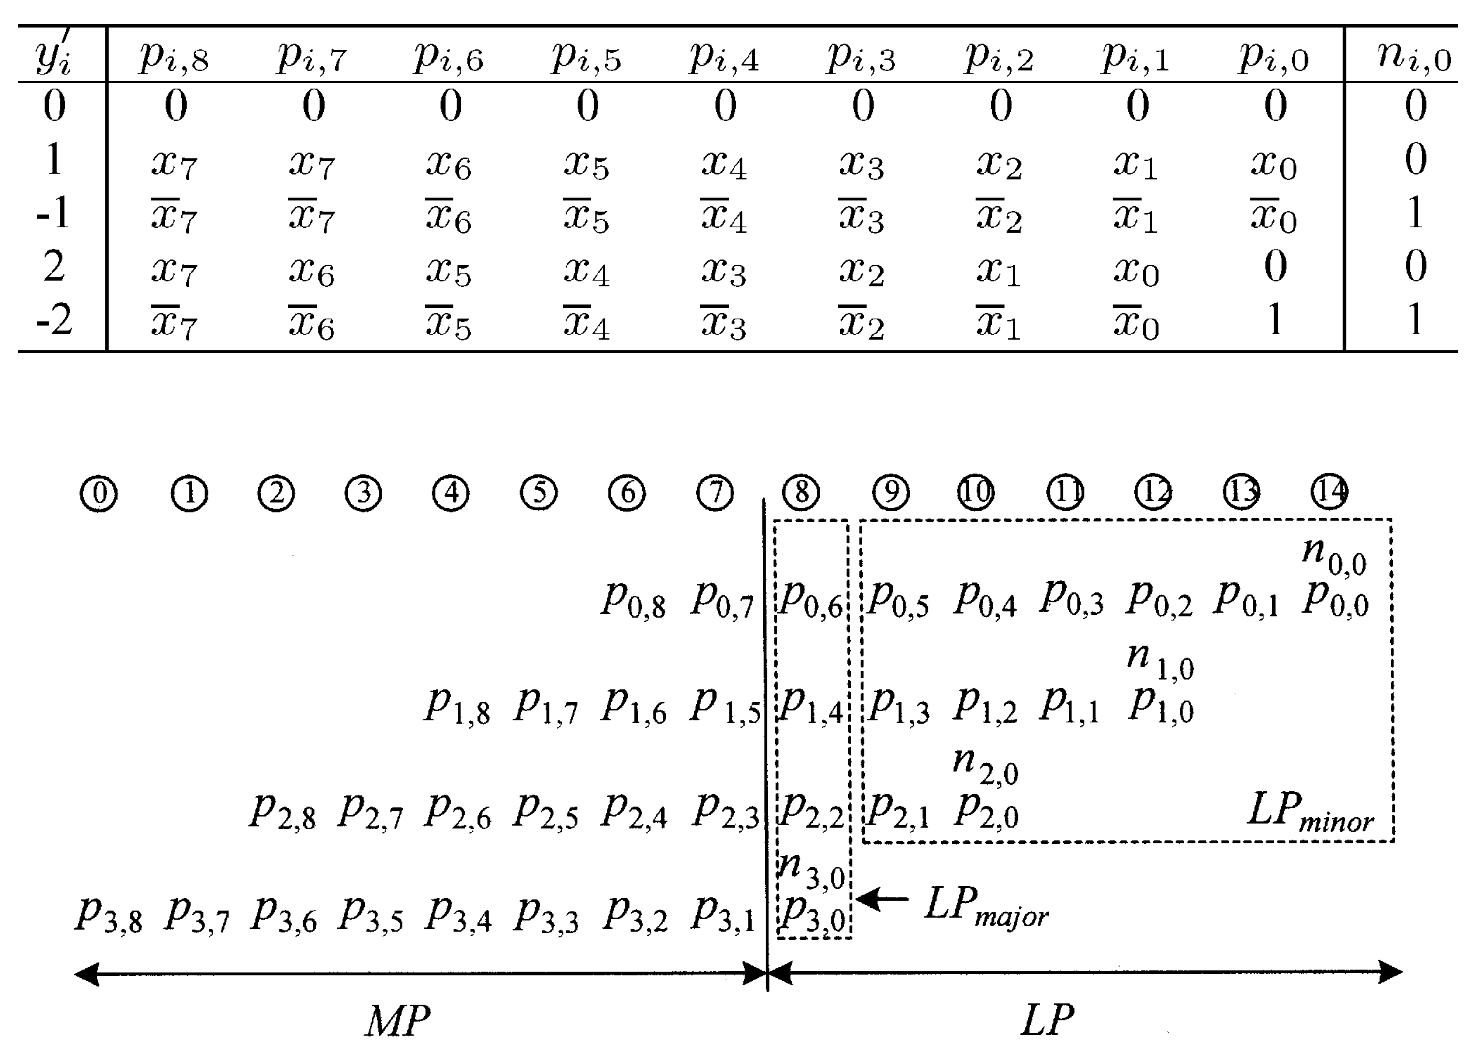
\includegraphics[width=0.6\linewidth]{00_chofixed.png}
    \caption{固定宽度改进 Booth 乘法器中保留部分与截断部分的划分框架\cite{cho2004fixedwidth}}
    \label{fig:related-fixedwidth}
\end{figure}

在固定宽度思想基础上，另一条重要路线利用操作数动态范围，将精确乘法转换为更小位宽的乘法加移位和加法。
Vahdat 等提出的 LETAM 将输入表示为二进制科学计数形式，仅保留高有效部分参与乘法运算\cite{vahdat2017letam}。
45 nm 工艺下相对精确乘法器，LETAM 的能量和面积分别改善 89.2\% 与 74.9\%，在 JPEG DCT 应用中 PSNR 下降仅 
0.15 dB\cite{vahdat2017letam}。后续的 AQ-LETAM 支持运行时精度切换，最高质量模式下功耗仍低精
确乘法器 79\%\cite{vahdat2017letam}，体现了从"单一近似点设计"向"可调近似机制设计"的演进。

在 LETAM 之后，Vahdat 等提出 TOSAM，结合前导 1 检测、截断和舍入策略，在 32 位乘法上
相对精确乘法器可实现约 95\% 的能量节省和 85\% 的面积节省，特定配置
下改进最高分别达 41\%、90\% 和 98\%\cite{vahdat2019tosam}。同时在 JPEG 和分
类任务中验证了有效性，PSNR/SSIM 下降控制在 1.39 dB 和 0.012 
以内\cite{vahdat2019tosam}。图~\ref{fig:related-tosam} 体现了 TOSAM 相对于其他结构的优势。

TOSAM 另一关键性质是误差分布近似高斯、均值接近零\cite{vahdat2019tosam}，这对累加型
计算尤为重要。带明显偏置的误差会在长链累加中持续漂移，而近零均值误差则更易被后续运算吸收。因
此 TOSAM 强调误差分布形态，将设计目标从"单点误差压缩"提升到"统计特性塑形"层面。

\begin{figure}[htbp]
    \centering
    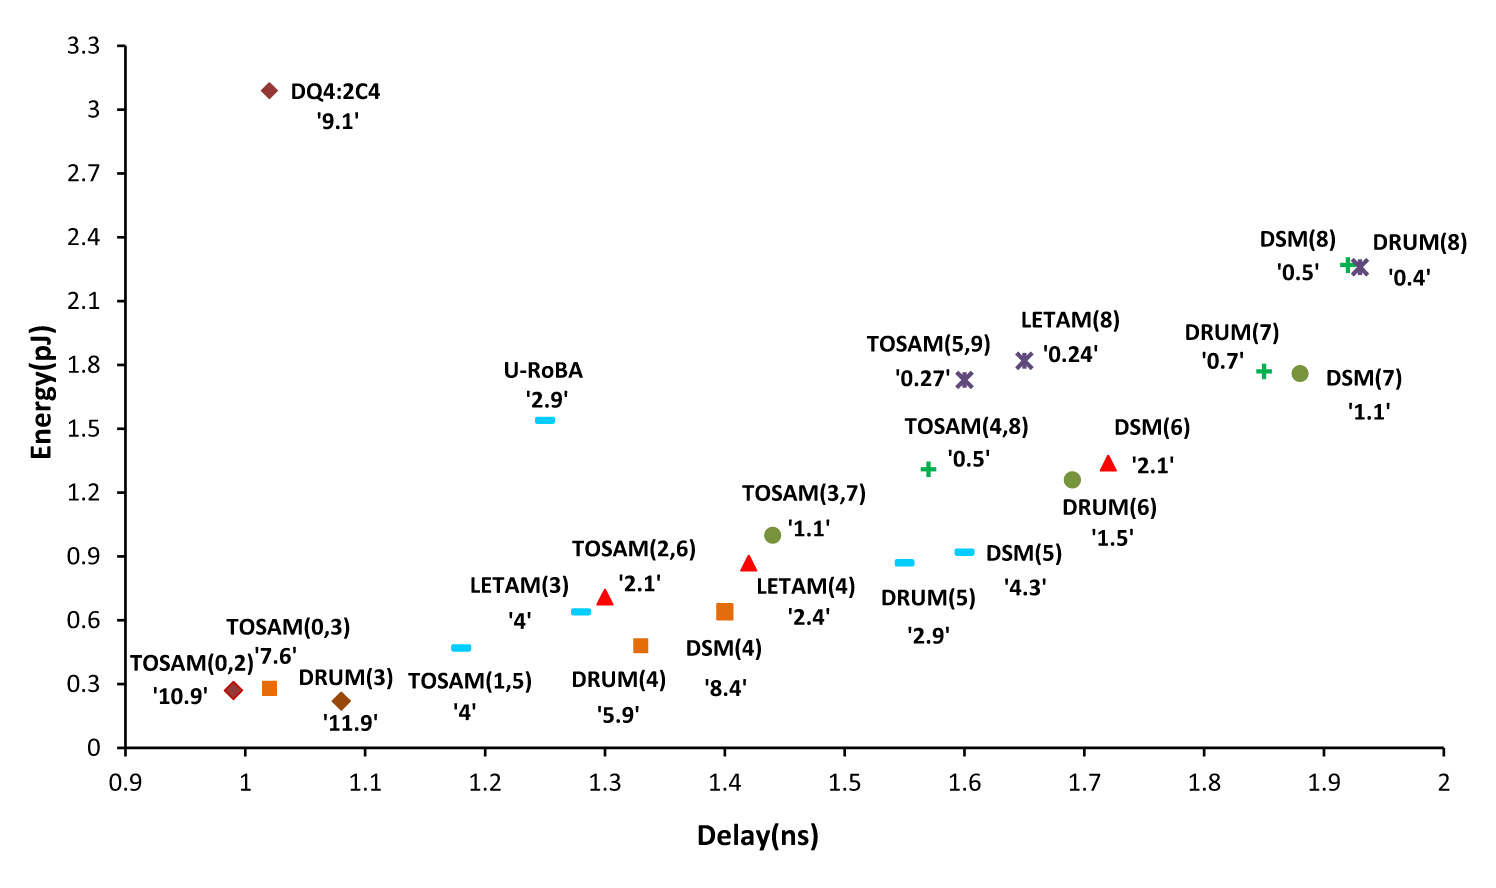
\includegraphics[width=0.6\linewidth]{01_tosam.png}
    \caption{TOSAM 与其他近似乘法器的延迟-能量对比\cite{vahdat2019tosam}}
    \label{fig:related-tosam}
\end{figure}

如果是固定宽度与动态截断路线侧重于“操作数处理”，Booth 类近似乘法器则直接针
对“部分积生成与压缩树结构”展开优化。Liu等在 Radix-4 架构下提出精简的近似编码器(R4ABE1与R4ABE2)，
大幅降低晶体管级复杂度和关键路径延迟，在 NMED 与 PDP 的折中中实现视觉质量保真\cite{liu2017radix4}。Qian
等多维度扩展该思路，设计 AWBM-II，融合近似编码、近似 4:2 压缩器及
规则化近似树，规避输出截断的前提下实现了可观的延迟与功耗改善，尤其利于适配阵列
型硬件加速\cite{qian2016wallacebooth}。

针对高基数(即Radix-8)架构下极大的预处理开销，Jiang 等基于近似2位
重编码加法器极大优化了硬件 PPA，并在 FIR 滤波器中论证了单一电路级误差无
法完全映射至系统输出的 SNR 表现\cite{jiang2016radix8}。与此互补，结构层面的
优化粒度进阶至极低错误概率($1/256$)的近似压缩器，Jaswal 等在手写分类与去噪任
务中以此取得显著功耗下降并保持高数据质量的成果，充分揭示了选择性精细化近似取代粗
粒度牺牲的方法优势\cite{jaswal2025approximate}。

横纵向对比可见，底层乘法设计逐渐析出两大具有特定应用意义的范式——通过前导位分离、
截断及移位加法的“算术等价重构”（如LETAM、TOSAM），其结构改动带来断崖式的能耗缩小但
敏感于操作数分布；以及对编码器与压缩树开刀的“局部逻辑近似”，较强可控性利于在高性能数据
流中嵌入。简而言之，即便底层 RTL 重构的 PPA 成绩已大步推进，目前依旧
亟待建立一个自硬件微结构、全状态误差特征穿透至后端应用级部署的完整分析流。


\subsubsection{面向神经网络的误差特征建模与近似映射}
随着近似乘法器逐步应用于神经网络推理，研究重心从“面积与功耗优化”转向“特定网络中的精度保持”。
传统误差指标如 NMED、MRED 等仅为统计汇总，未能反映权值分布、激活分布及误差放大机制，导致电路
级指标与网络精度表现不一致。Jiang 等在 FIR 场景中发现，NMED 较大的设计并不一定导致系统输出
 SNR 更差\cite{jiang2016radix8}，促使研究进入“误差-应用映射”阶段。

Mo 等构建了包含 1200 余种近似乘法器的大规模库，分析 16 个统计误差特征与神经网络准确
率退化的关联，发现误差偏置 $\mu E$、平均误差距离 $\mu ED$ 和错误率 ER 的组合最为
关键\cite{mo2024learning}。基于此构建的分类模型在大多数应用中达到 96\%--99\% 的 top-1 
分类精度，若允许 3\% 的准确率损失，正确分类概率超过 96\%\cite{mo2024learning}。此外，研究
表明，较小的 $\mu E$ 并不足以保证网络精度，还需限制 $\mu ED$ 和 ER 的绝对值，否则误差可能在累加
中放大。图~\ref{fig:related-errorfeatures} 展示了误差特征与应用精度的关系框架。

该研究还提出以 3\% 和 8\% 的准确率损失为分界，将近似乘法器划分为不同类别\cite{mo2024learning}，更
贴近实际设计流程。通过分阶段缩减设计空间，避免了“先综合、再仿真”的低效流程。进一步分析显示，在 VGG16-CI
FAR10 场景下，若允许 3\% 的准确率损失，部分乘法器可实现 21.88\% 的 PDP 改进和 27.52\% 的 ADP 改进；若允许
再训练，收益可超过 40\%\cite{mo2024learning}。

\begin{figure}[htbp]
    \centering
    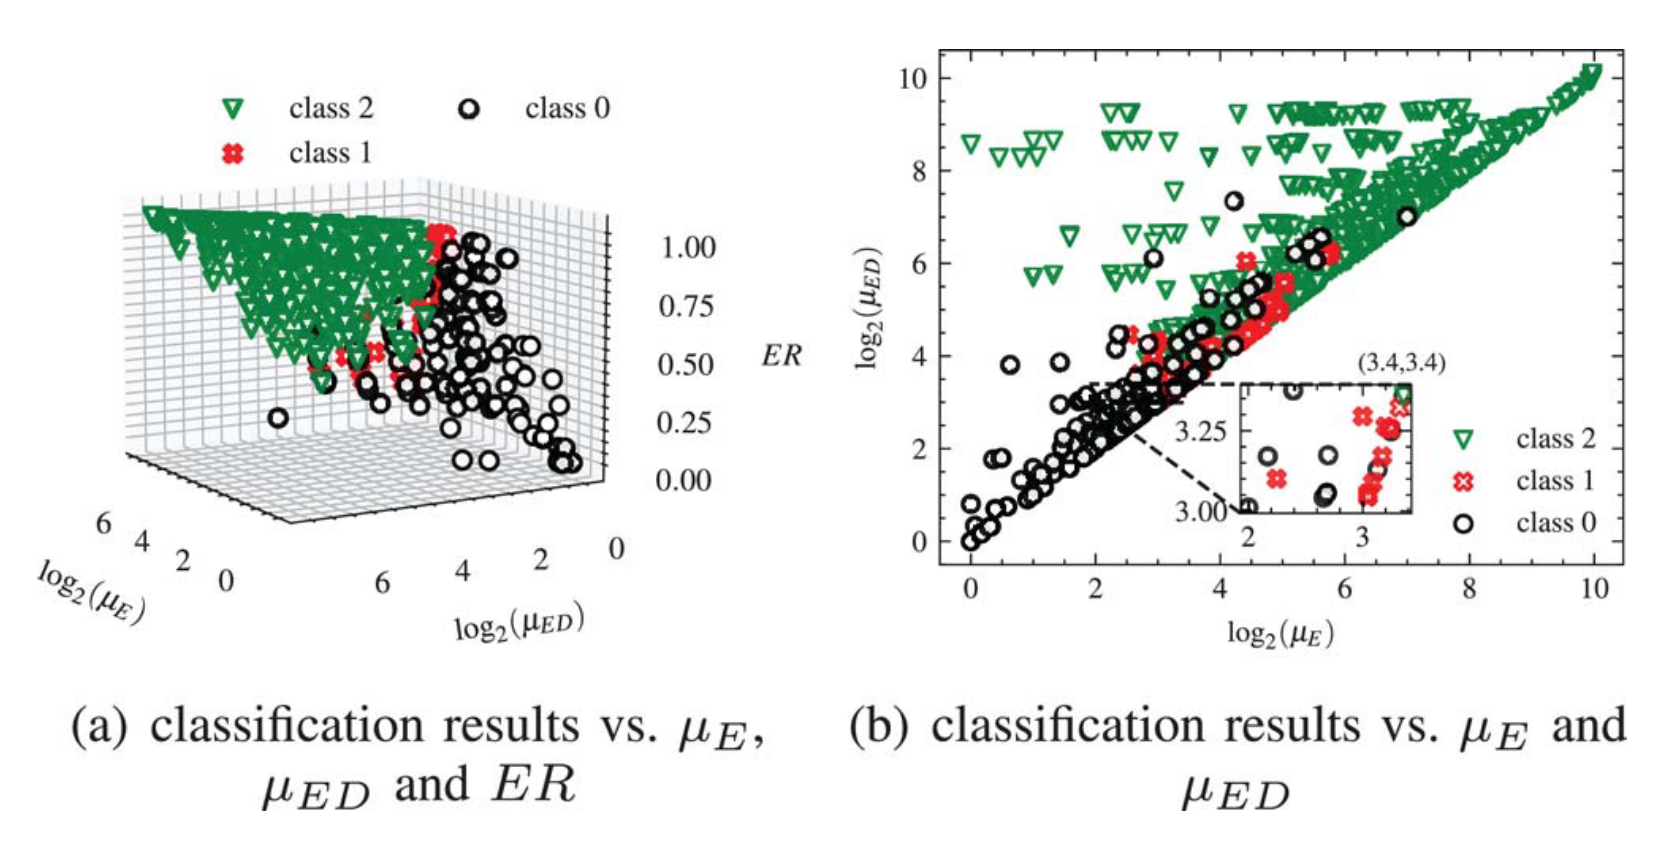
\includegraphics[width=0.6\textwidth]{03_molearning.png}
    \caption{近似乘法器误差特征与神经网络应用精度退化关系图\cite{mo2024learning}}
    \label{fig:related-errorfeatures}
\end{figure}

上述研究改变了近似乘法器的评价方式，从关注“功耗降低”转向“应用精度约束下的筛选”。
Danopoulos 等提出基于 PyTorch 的近似仿真框架 TransAxx，结合硬件驱动的 MCTS 搜索，
优化 Vision Transformer 的分层近似配置，在精度差异小于 1\% 的条件下，功耗平均降低 21\%\cite{danopoulos2025transaxx}。
该研究表明，不同层对误差的敏感度差异显著，统一替换策略正被更精细的层级映射取代。

从方法论看，近似计算正从“结构设计”转向“结构-模型共同优化”。乘法器不再是静态部件，而是可根据层位置、
数据分布和精度预算动态调度的资源。

\subsubsection{面向Transformer加速器的数据流与系统协同优化}

当研究对象从卷积网络扩展到 Transformer 时，近似计算的重点转向数据流与存储优化。
Lee 等分析 BERT-Large 应用发现，自注意力模块延迟占比随序列长度增加显著上升\cite{lee2023hammer}。
基于注意力概率的长尾分布特性，提出 mean-redistribution 和线性化近似机制，用移位与加法替代复杂计算，
性能提升 1.2--1.6$\times$，能效提升 1.2--1.5$\times$，面积减少 27\%\cite{lee2023hammer}。图~\ref{fig:related-hammer} 
展示了延迟分解框架。

\begin{figure}[htbp]
    \centering
    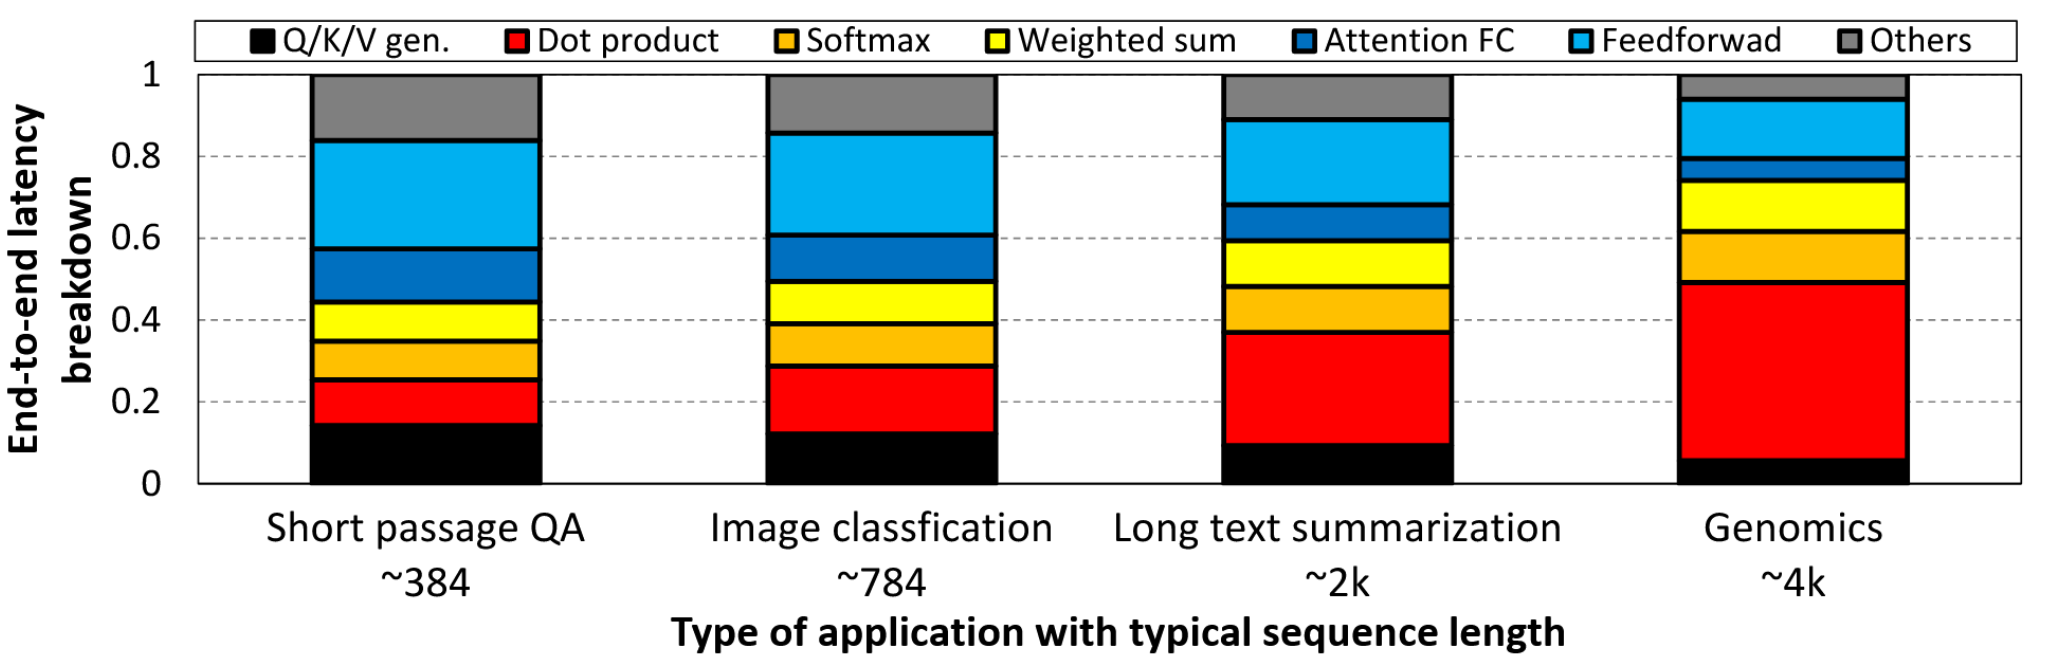
\includegraphics[width=0.6\textwidth]{04_hammer.png}
    \caption{Transformer 应用中自注意力模块的延迟占比分解图\cite{lee2023hammer}}
    \label{fig:related-hammer}
\end{figure}

如果说 HAMMER 主要解决“注意力计算更便宜”，Han 等的 TranSIC 则聚焦“权
重搬移更少”\cite{han2026transic}。该研究指出，Transformer 加速器中权重搬移
能耗占比高达 37.54\%，提出 storage in computing（SIC）方法，将权重矩阵嵌入计算电
路，避免频繁读取。实验显示，TranSIC 能效提升最高 56.24$\times$，吞吐提升 9.81$\times$，数据
搬移次数减少 42.98\%，能耗降低 45.49\%\cite{han2026transic}。图~\ref{fig:related-transic} 展
示了数据搬移与能耗分解框架。

\begin{figure}[htbp]
    \centering
    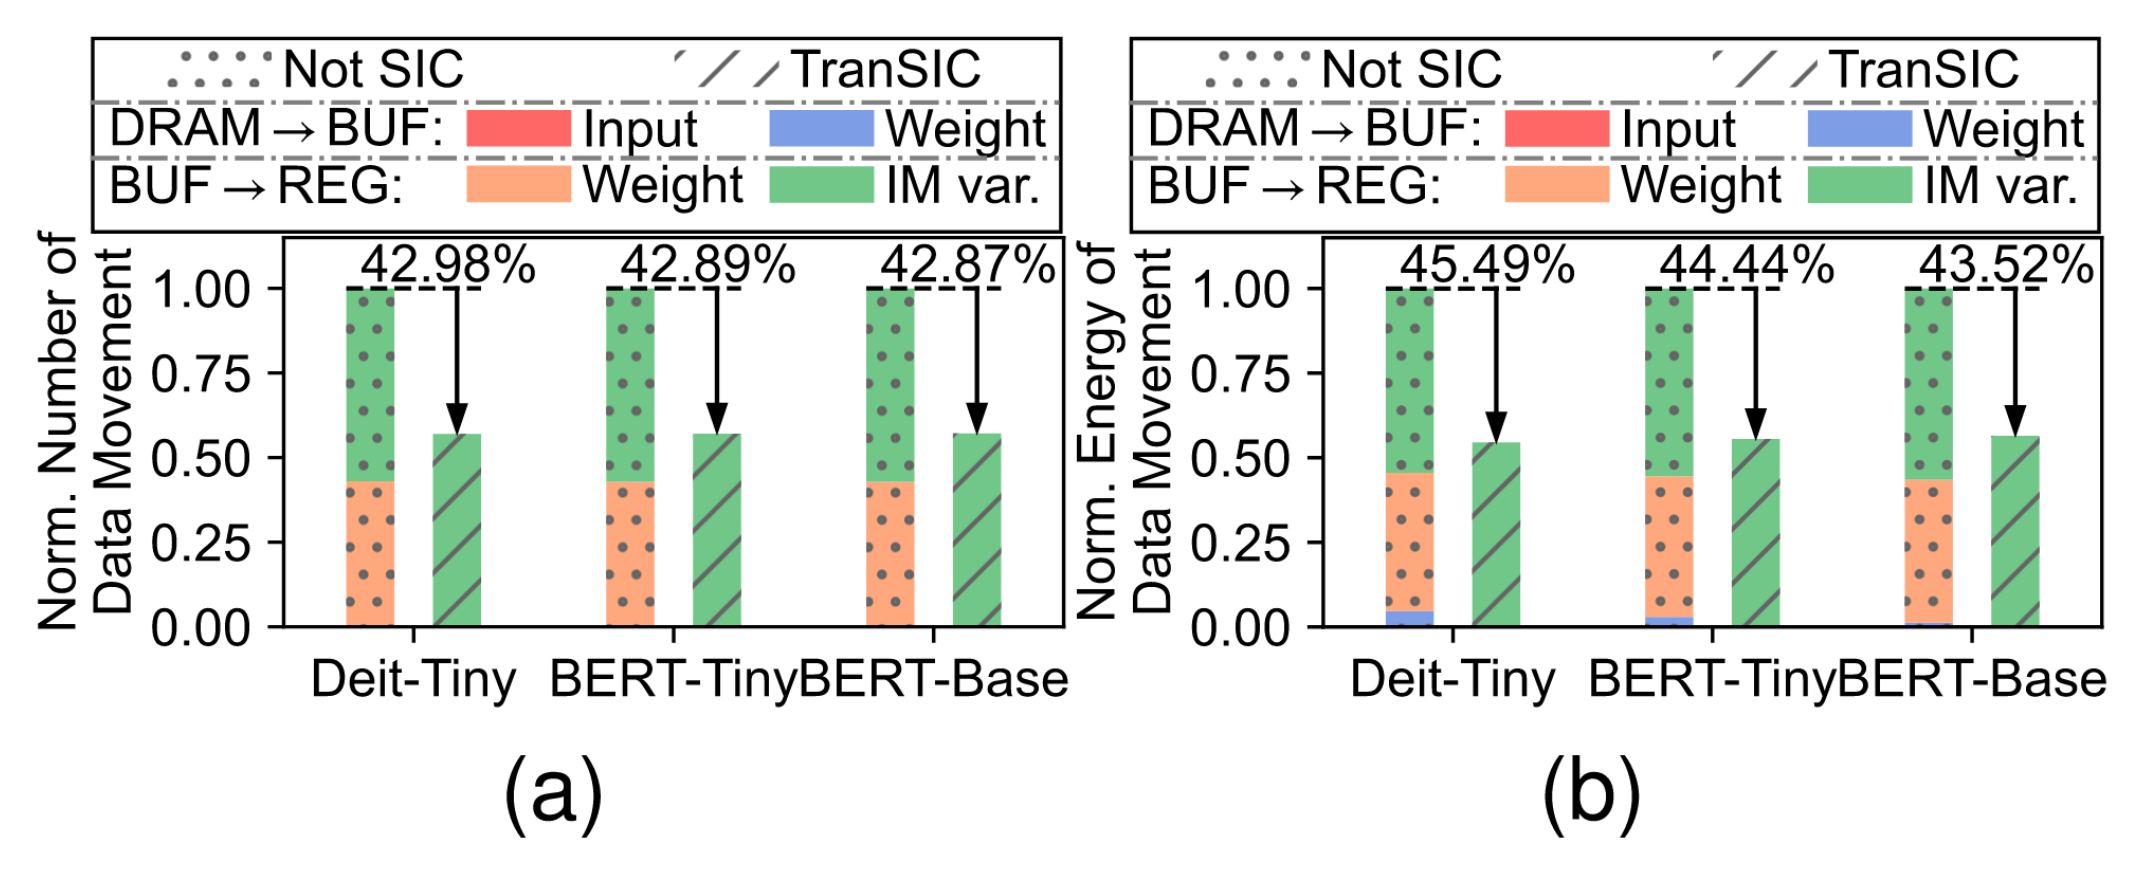
\includegraphics[width=0.6\textwidth]{05_hantransic.png}
    \caption{Transformer 加速器中数据搬移数量与能耗分解图\cite{han2026transic}}
    \label{fig:related-transic}
\end{figure}

应当指出，已有工作开始将近似计算拓展至 ViT 及更大规模模型，
但多属趋势性补充而非本文核心。例如，TransAxx 指出近似乘法器的
选型需与层级敏感性、量化和再训练联动考虑\cite{danopoulos2025transaxx}；MSDM 通过基
于最高有效位的移位乘法，在单元级实现约 28.31\% 面积缩减、57.84\% 功耗下降和 11.86\% 延迟改善，
并在若干 DNN 任务中达成约 60\% 的能量节省且精度近乎无损\cite{gong2024msdm}。总体来看，这些成果
表明近似乘法器正与量化、层级搜索及专用阵列协同发展，但研究多数聚焦于特定模型或 GEMM 数据通路的定
制优化，而非面向通用张量加速器的可复用近似乘法器 IP 的系统化集成。

\subsection{本文主要研究内容}
本文围绕“近似乘法器设计 - 误差机理分析 - 加速器系统集成 - 应用级验证”四个层面展开，
主要研究内容如下：

第一，完成三类代表性近似乘法器的复现、参数化设计与对比实现，包括 TOSAM、ZBA-BM 与 LETAM，
并结合 RTL 与 Chisel 两种实现路径，形成可配置位宽、近似深度与精度模式的通用算子 IP。

第二，面向算子级误差机理开展系统分析，围绕全输入空间误差统计、误差分布特征刻画与不同配置下的
鲁棒性变化进行建模；针对 Booth 类近似中 Row-0 引入的固有偏差，提出选择性部分积补偿机制，
使 ZBA-BM 在不同近似深度下保持零均值误差，并与 TOSAM 的低方差特性、LETAM 的动态位宽重构能力
共同构成可比较的近似设计谱系。

第三，围绕硬件实现与工程化优化，对上述算子开展 45\,nm 逻辑综合、7\,nm 跨工艺 PPA 映射与面积、
功耗、时延权衡分析，进一步明确不同近似策略在电路层面的成本边界和适用场景。

第四，将近似乘法器路径集成到 Chipyard/Gemmini 生成器中，完成 Scala 适配、系统级仿真与软硬件协同
验证，并在裸机矩阵乘、ResNet-50 \texttt{conv1} 与 TinyLlama 困惑度评估等任务上进行应用级测试，
从而建立从算子、阵列到模型推理的跨层验证链路。

通过上述工作，本文形成了可复用近似乘法器 IP、误差刻画方法与加速器集成方案的完整闭环，
为面向大语言模型推理的低能耗矩阵乘法设计提供了可实现、可验证且可迁移的技术基础。

\clearpage
\section{近似乘法器算子架构分析}

为系统评估近似乘法器在矩阵乘法通路中的适用性与误差特性，
本研究选取三种具有代表性的近似乘法器架构进行复现、参数化实现与对比优化：
TOSAM（基于前导位检测的截断与舍入策略）、Radix‑8 Booth（针对部分积生成与压缩树的
局部逻辑近似）以及 LETAM（基于二进制科学计数的动态位宽重构）。
本节将详细介绍这三种架构的算法原理、硬件架构以及可配置精度设计，
为后续的 RTL 实现与系统集成奠定基础。

\subsection{TOSAM：一种基于截断与舍入的节能型可扩展近似乘法器}
TOSAM（Truncation- and Rounding-Based Scalable Approximate Multiplier）由 Vahdat 等提出，
其核心目标不是在部分积压缩树或末级加法器中局部引入近似，而是直接从操作数表示方式入手，
利用前导“1”位置对输入动态范围进行重构，从而将原本完整的 $n$ 位乘法转化为“移位 + 截断加法 + 
小位宽乘法”的组合运算\cite{vahdat2019tosam}。
一方面，近似乘法核心的规模主要由参数 $h$ 和 $t$ 决定，而与原始操作数字长弱相关，
因此具有良好的可扩展性；另一方面，通过在截断基础上进一步引入舍入，TOSAM 将误差分
布调整为近似高斯且均值接近零的形态，使其更适合后续累加型计算。

TOSAM 的算法基础是将正整数重新写成以前导“1”为基准的二进制科学计数形式。
对于任意正整数 $N$，设其最高有效“1”位位置为 $k$，则有
\begin{equation}
N=\sum_{i=0}^{k}2^{i}x_i ,
\label{eq:tosam_n}
\end{equation}
进一步提出公因子 $2^k$，可得
\begin{equation}
N=2^k\left(\sum_{i=0}^{k}2^{i-k}x_i\right)=2^k X ,
\label{eq:tosam_x}
\end{equation}
其中 $X\in[1,2)$。若两个输入操作数分别为 $A$ 和 $B$，则精确乘法可表示为
\begin{equation}
A\times B = 2^{k_A+k_B}X_A X_B .
\label{eq:tosam_exact}
\end{equation}
式~\eqref{eq:tosam_exact} 的难点在于 $X_A$ 与 $X_B$ 仍保持接近原输入位宽，因而 $X_A X_B$ 仍然昂贵。为此，原文定义
\begin{equation}
Y = X-1,
\label{eq:tosam_y}
\end{equation}
使得 $Y\in[0,1)$，从而将乘法问题改写为对分数部分的近似处理。

\begin{figure}[htbp]
    \centering
    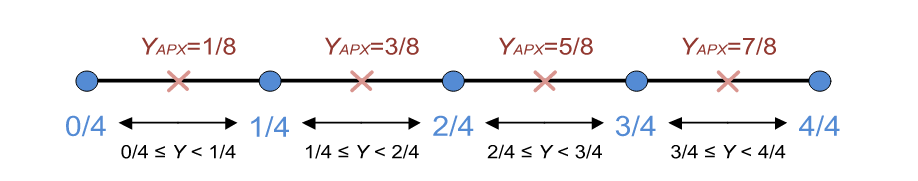
\includegraphics[width=0.8\textwidth]{06_TOSAM1.png} 
    \caption{TOSAM 中分数项 $Y$ 的分段近似示意图\cite{vahdat2019tosam}}
    \label{fig:tosam-seg}
\end{figure}

设分段数为
\begin{equation}
S=2^h,
\label{eq:tosam_s}
\end{equation}
其中 $h$ 为控制近似精度的设计参数。原文将 $Y$ 的近似值定义为各区间的中值，即
\begin{equation}
Y_{\mathrm{APX}}=\frac{2m-1}{2S}, \qquad \frac{m-1}{S}\le Y < \frac{m}{S}, \quad m=1,2,\ldots,S.
\label{eq:tosam_yapx}
\end{equation}
这一表达式的硬件含义非常重要：为了得到 $Y_{\mathrm{APX}}$，并不需要完整的比较器和查找表，只需截取 $Y$ 的前 $h$ 位，再在截断结果右侧补入一个恒为“1”的最低位即可。这意味着 $Y_{\mathrm{APX}}$ 的生成本质上是“截断 + 固定舍入”，而非一般意义上的复杂量化过程。将式~\eqref{eq:tosam_y} 代回式~\eqref{eq:tosam_exact}，精确乘法可写为
\begin{equation}
A\times B = 2^{k_A+k_B}\left(1+Y_A+Y_B+Y_A Y_B\right).
\label{eq:tosam_expand}
\end{equation}
为了进一步降低硬件成本，TOSAM 并不保留完整的 $Y_A$ 和 $Y_B$，而是仅保留其前 $t$ 位，分别记为 $(Y_A)_t$ 和 $(Y_B)_t$，同时用更短位宽的 $(Y_A)_{\mathrm{APX}}$ 与 $(Y_B)_{\mathrm{APX}}$ 近似乘法项。于是最终的近似结果为
\begin{equation}
(A\times B)_{\mathrm{APX}}
\approx
2^{k_A+k_B}
\left(
1+(Y_A)_t+(Y_B)_t+(Y_A)_{\mathrm{APX}}(Y_B)_{\mathrm{APX}}
\right).
\label{eq:tosam_final}
\end{equation}
式~\eqref{eq:tosam_final} 就是 TOSAM 的核心算法。
它对应的结构含义是：原始 $n\times n$ 乘法已被分解为一个由常数项、
两个截断分数项以及一个 $(h+1)$ 位小乘法项构成的计算核，再整体左移 $k_A+k_B$ 位即可得到结果。

从硬件实现角度看，TOSAM 的数据通路具有非常清晰的模块边界。
其第一个关键模块是 Approximate Absolute Unit，
用于在有符号场景下快速生成输入的近似绝对值；
作者并未采用完全精确的补码求绝对值，而是复用了早期工作的近似绝对值电路，
以避免在输入预处理阶段重新引入较长关键路径\cite{vahdat2019tosam}。
第二个关键模块是 Leading-One Detector Unit，用于找出 $|A|_{\mathrm{app}}$ 与 $|B|_{\mathrm{app}}$ 
的前导“1”位置，并生成 $k_A$、$k_B$ 以及相应 one-hot 形式的检测信号。原文给出的逻辑形式为
\begin{equation}
K[i] = \left(\bigwedge_{j=i+1}^{n-2}\overline{I[j]}\right)\wedge I[i], \qquad 0\le i \le n-2,
\label{eq:tosam_lod}
\end{equation}
其中 $I$ 表示输入绝对值向量。该式表明，只有当前位为“1”且其更高位全为“0”时，$K[i]$ 才为真。第三个关键模块是 Truncation Unit，它依据前导位位置，从标准化后的分数项中提取 $(Y_A)_t$ 和 $(Y_B)_t$。原文给出的位级关系为
\begin{equation}
(Y)_t[i] = \bigvee_{j=0}^{n-2}\left(K[j]\wedge I[j+i-t]\right), \qquad i<t.
\label{eq:tosam_trunc}
\end{equation}
式~\eqref{eq:tosam_trunc} 的本质是按前导位位置完成“对齐后截断”，从而避免显式移位桶形器。接下来的 Arithmetic Unit 完成式~\eqref{eq:tosam_final} 中括号部分的求和与小位宽乘法，且 $(Y_A)_{\mathrm{APX}}$ 与 $(Y_B)_{\mathrm{APX}}$ 可以由 $(Y_A)_t$ 和 $(Y_B)_t$ 直接布线生成，无需额外复杂逻辑。最后，Shift Unit 完成整体左移 $k_A+k_B$，Sign and Zero Detector Unit 负责恢复结果符号并处理零输入情况。按照原文的实现流程，unsigned 版本只需删去近似绝对值与符号恢复模块即可\cite{vahdat2019tosam}。

\begin{figure}[htbp]
    \centering
    \begin{subfigure}[b]{0.49\textwidth}
        \centering
        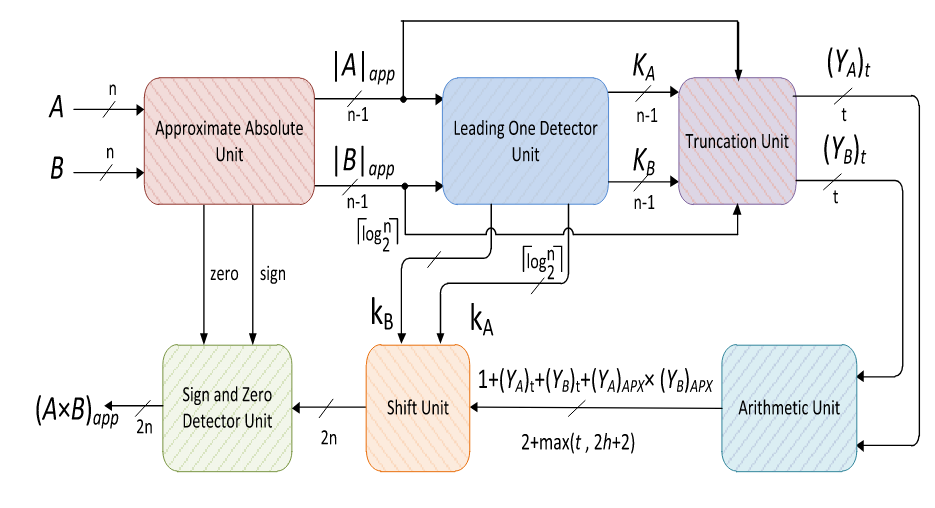
\includegraphics[height=4.0cm]{06_TOSAM4.png}
        \caption{TOSAM 有符号实现的总体硬件框图\cite{vahdat2019tosam}}
        \label{fig:tosam-arch}
    \end{subfigure}\hfill
    \begin{subfigure}[b]{0.49\textwidth}
        \centering
        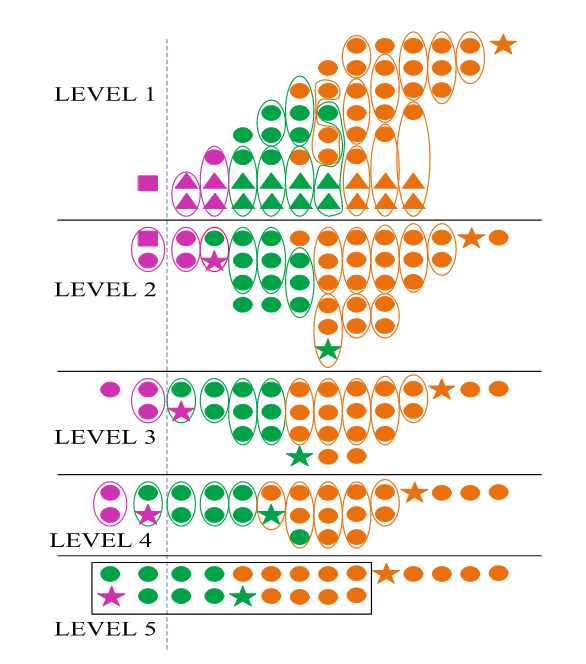
\includegraphics[height=4.0cm]{06_TOSAM6.png}
        \caption{TOSAM 不同精度模式下的归约结构\cite{vahdat2019tosam}}
        \label{fig:tosam-config}
    \end{subfigure}
    \caption{TOSAM 的硬件架构与可配置精度设计}
    \label{fig:tosam-pair}
\end{figure}

为支持运行时精度切换，原文提出 accuracy‑configurable TOSAM，在单一硬件中实现多组 $(h,t)$ 配置，并通过功耗门控与布线复用在模式
间切换\cite{vahdat2019tosam}。32 位可配置实现包含三种模式：T2、T6 与 T9，分别对应 TOSAM$(0,2)$、$(2,6)$ 和 $(5,9)$。Truncation 
与 Shift 单元按最大 $h,t$ 配置实现，Arithmetic 单元通过 power‑gating 在低精度模式下削减部分积与归约级，低位结果由传输门置零或旁路输
出（见图~\ref{fig:tosam-config}）。原文误差分
析指出：当 $h>0$ 时 $t=h+4$ 在精度、速度与能耗
间较优；$h=0$ 时 $t=3$ 对应最小 MARE\cite{vahdat2019tosam}。该经验
可沿 $t=h+4$ 轨迹简化参数搜索，显著降低探索成本。

\subsection{ZBA-BM：基于 K-Map 化简与 Row-0 选择性部分积补偿的零偏差 Booth 近似乘法器}
\label{subsec:zbabm-arch}

ZBA-BM（Zero-Bias Approximate Booth Multiplier）以~\cite{liu2017radix4}~所提 Radix-4 近似 Booth 乘法器（R4ABE2）为基线设计：该方案通过 $\pm 2A \to \pm A$ 的近似代换与部分积生成逻辑化简，相对精确 Radix-4 Booth 显著压缩门级面积，但在乘法器阵列首行（Row-0）因物理边界条件残留 $\mu = -0.125$ 的系统偏差。本工作在 R4ABE2 之上自主创新地引入 Row-0 选择性部分积补偿（PPSC）机制，以局部硬件支路将首行偏差期望归零，同时保留 R4ABE2 的全部面积与功耗节省。后续依次给出：$\pm 2A$ 近似代换、K-Map 逻辑化简与零编码守恒项、Row-0 偏差溯源、PPSC 机制与综合后端处置。

\subsubsection{Radix-4 Booth 编码与 $\pm 2A$ 近似代换}

考虑两个 $N$ 位补码表示的有符号数：被乘数 $A$ 与乘数 $B$，可分别展开为
\begin{equation}
\label{eq:zbabm_a_expand}
A = -a_{N-1}\,2^{N-1} + \sum_{j=0}^{N-2} a_j\,2^j ,
\end{equation}
\begin{equation}
\label{eq:zbabm_b_expand}
B = -b_{N-1}\,2^{N-1} + \sum_{i=0}^{N-2} b_i\,2^i .
\end{equation}
在标准 Radix-4 Booth 编码中，
乘数 $B$ 被划分为 3 位重叠滑动窗口
\(\{b_{2i+1}, b_{2i}, b_{2i-1}\}\)，
记为 $B_W$，并映射到集合 $\{-2,-1,0,1,2\}$。
该映射将部分积行数减半，
但需要支持 $\pm 2A$ 操作，
对应额外的移位与多路复用电路。

为精确表达 $\pm 2A$ 项，传统 Booth 部分积生成器需要复用器与移位电路。
若将 $\pm 2A$ 映射简化为 $\pm A$，可省略相应的控制逻辑门。
表~\ref{tab:zbabm_approx_map} 给出这一近似映射规则：
以幅度精度为代价换取门级面积的压缩。

\begin{table}[htbp]
\centering
\caption{$\pm 2A \to \pm A$ 幅度近似映射}
\label{tab:zbabm_approx_map}
\small
\begin{tabular}{c|c|c|c}
\toprule
$b_{2i+1} b_{2i} b_{2i-1}$ & Booth 选通 & 精确输出 & 近似输出（去 $2A$） \\
\midrule
0 0 0           & $0$  & $0$    & $0$    \\
0 0 1 \& 0 1 0  & $+1$ & $+A$   & $+A$   \\
0 1 1           & $+2$ & $+2A$  & $+A$ \\
1 0 0           & $-2$ & $-2A$  & $-A$ \\
1 0 1 \& 1 1 0  & $-1$ & $-A$   & $-A$   \\
1 1 1           & $0$  & $0$    & $0$    \\
\bottomrule
\end{tabular}

\smallskip
\footnotesize{\textit{$2A \to A$ 简化省略了对应的复用门，代价是 011 与 100 编码的输出相对精确值偏离 $\pm A$。}}
\end{table}

\subsubsection{K-Map 逻辑化简与零编码守恒项}

在门级拓扑（如 R4ABE2~\cite{liu2017radix4}）中，
该简化将原本多级 NAND、NOR 嵌套的控制树压缩为单层 XOR/AND 门组合，
编码器晶体管数减少约 80\%。
为系统化分析简化后的部分积逻辑，
本文以 $a_j a_{j-1}$ 与编码窗 $B_W$ 为坐标构建二维卡诺图，
如表~\ref{tab:zbabm_kmap} 所示。
该图穷举了 $B_W$ 与 $a_j a_{j-1}$ 所有组合下的 $pp_j$ 取值。

\begin{table}[htbp]
\centering
\caption{ZBA-BM 部分积 $pp_j$ 的二维卡诺图}
\label{tab:zbabm_kmap}
\resizebox{0.95\columnwidth}{!}{%
\begin{tabular}{c|cccccccc}
\toprule
\diagbox{$a_j a_{j-1}$}{$b_{2i+1} b_{2i} b_{2i-1}$} & 000 & 001 & 011 & 010 & 110 & 111 & 101 & 100 \\
\midrule
00 & 0 & 0 & 0 & 0 & 1 & 0 & 1 & 1 \\
01 & 0 & 0 & \textcircled{\scriptsize 0} & 0 & 1 & 0 & 1 & \textcircled{\scriptsize 1} \\
11 & 0 & 1 & 1 & 1 & 0 & 0 & 0 & 0 \\
10 & 0 & 1 & \textcircled{\scriptsize 1} & 1 & 0 & 0 & 0 & \textcircled{\scriptsize 0} \\
\bottomrule
\end{tabular}}

\smallskip
\footnotesize{\textit{圈注 \textcircled{\scriptsize 0} / \textcircled{\scriptsize 1} 标记由于 $\pm 2A \to \pm A$ 简化在该格上发生的逆变。}}
\end{table}

观察表~\ref{tab:zbabm_kmap}：上下半区的 $pp_j$ 取值分布关于中心边界对称，
说明 $pp_j$ 与 $a_{j-1}$ 解耦。
当 $a_j = 1$（下半区），$pp_j = 1$ 当且仅当 $b_{2i+1}$（即极性标志 \texttt{neg}）等于 0，
且 $B_W$ 不属于 $\mathtt{000}$ 或 $\mathtt{111}$ 的零编码（即 $\neg\mathtt{zero}$）。
依据卡诺图圈组化简，部分积可表达为单解析式：
\begin{equation}
\label{eq:zbabm_pp}
pp_j \;=\; \neg\mathtt{zero} \,\land\, (a_j \oplus \mathtt{neg}) .
\end{equation}
该解析式仅需 1 个 AND 门与 1 个 XOR 门即可生成单比特部分积。
$\neg\mathtt{zero}$ 称为零编码守恒项，不可省略：
若擦除该项以进一步压缩面积，
当 $B_W = \mathtt{111}$（精确为零）时，
$a_j \oplus \mathtt{neg}$ 仍可触发 $0\oplus 1 = 1$ 反转，
使整行部分积变为 $\mathtt{1\dots 1}$，
增加加法树的无效翻转活动，破坏低功耗目标。

\subsubsection{Row-0 系统偏差溯源}

标准 Radix-4 Booth 编码在统计意义上无偏。
但在乘法器阵列首行（Row-0，$i=0$），
$b_{-1}$ 因物理边界条件被置 0，
编码窗坍缩为 $\{b_1, b_0, 0\}$，
使 \texttt{011} 编码的出现概率为 0。
在精确实现下此截断不影响输出；
引入 $\pm 2A \to \pm A$ 的近似后则破坏了误差对称性。
本文以误差 $=$ 精确值 $-$ 近似值为符号约定：
编码 \texttt{100}（精确对应 $-2A$）出现概率为 $1/4$，
被近似为 $-A$，产生 $-A$ 的误差；
其他行中该 $-A$ 误差可由 \texttt{011}（精确对应 $+2A$，被近似为 $+A$）的 $+A$ 误差抵消，
但 Row-0 中 \texttt{011} 概率为 0，正向补偿缺失。
Row-0 整体误差期望因此固化为
\begin{equation}
\label{eq:zbabm_mu_row0}
\mu_{\text{row-0}} \;=\; -\tfrac{1}{8} \;=\; -0.125 ,
\end{equation}
这是 ZBA-BM 偏差级联现象的微架构来源。

\subsubsection{Row-0 选择性部分积补偿（PPSC）}
\label{subsubsec:zbabm_ppsc}

既有的常数偏差消除方案以增加操作数为代价，
通常需要取反器矩阵或扩展加法树宽度。
本文提出 Row-0 选择性部分积补偿（Partial-Product Selective Compensation at Row-0, PPSC）：
在 Row-0 的部分积生成路径中并联一条局部补偿支路，
仅在 $B_W = \mathtt{100}$ 时启用，从源头消除 $\mu$。
具体地，
\begin{equation}
\label{eq:zbabm_ppsc}
pp_j^{\text{Row-0}} \;=\;
\begin{cases}
a_{j-1}, & \text{若 } i = 0 \,\land\, B_W = \mathtt{100}, \\
\neg\mathtt{zero} \land (a_j \oplus \mathtt{neg}), & \text{其他}.
\end{cases}
\end{equation}
在 Row-0 的每一比特部分积位置并联一个 2:1 MUX：
当 $i = 0$ 且 $B_W = \mathtt{100}$ 时，
MUX 在第 $j$ 位输出 $a_{j-1}$，
等价于将 $A$ 整体左移一位，
从而恢复精确的 $-2A$ 部分积；
其他场景仍走全展开 K-Map 通道。
补偿支路与部分积阵列旁路并联，不进入压缩树反馈，
关键路径与 K-Map 通道相互独立，
不增加 Dadda 树高度（$h=4$）。
图~\ref{fig:zbabm_kmap_flat} 给出 PPSC 的硬件拓扑：
全展开 K-Map 通道与 Row-0 局部补偿支路在部分积阵列中并列，
将 Row-0 偏差期望归零至 $\mu = 0$。

\begin{figure}[htbp]
\centering
\includegraphics[width=\textwidth]{PicDoc/PicDoc_2026-04-28+20_12_36.png}
\caption{近似 Booth 乘法器结构演化与 ZBA-BM 的 PPSC 机制}
\label{fig:zbabm_kmap_flat}
\end{figure}

\paragraph*{$N/2+1$ 行溢出与综合后端处置.}
8 位 Radix-4 Booth 乘法在第 6 位会出现 4 行部分积全占的 Dadda 高度 5 问题：
负向部分积的符号扩展位 $\mathtt{neg\_bits}_3$ 无法纳入主部分积阵列，
只能以稀疏第 5 操作数的形式外挂，
触碰了 Radix-4 Booth 的经典 $N/2+1$ 行溢出问题\cite{goto1992np1overflow,kuang2010modified}。
本文采取的解法是保持稀疏外挂、由综合后端自动调度：
保留 $(\mathtt{neg\_bits}_3 \!\ll\! 6)$ 为独立稀疏操作数，
依靠 Synopsys Design Compiler 的 \texttt{compile\_ultra} 调度其内部 3:2 压缩器；
该位生成早于主部分积阵列，
综合后端可将其接入快速引脚，使 Fmax 不被 $N/2+1$ 外挂行主导（实证见 §\ref{subsec:ppa}）。

\subsection{LETAM：面向低能耗的截断型可配置精度近似乘法器架构}

LETAM（Low Energy Truncation-Based Approximate Multiplier）由Vahdat等提出\cite{vahdat2017letam}，其核心思想为直接从操作数的二进制科学计数表示入手，通过截断分数部分与部分积剪枝，将完整的$n$位乘法降维为移位、加法与小位宽乘法的组合，从而在保持较高精度的前提下实现功耗与延迟的显著降低。相较于传统的动态段方法（DSM）和静态段方法（SSM），LETAM引入了两个独立的截断参数以实现更精细的精度-面积权衡。

原始LETAM的近似计算公式为
\begin{equation}
A \times B \approx 2^{k_A+k_B} \left( 1 + (X_A)_{t'} + (X_B)_{t'} + \mathrm{trunc}((X_A)_t \times (X_B)_t) \right)
\label{eq:original_letam}
\end{equation}
其中$(X)_t$表示截取$X$的高$t$位，$\mathrm{trunc}(\cdot)$表示截断操作。原始LETAM的核心计算为截断加法和剪枝小乘法。

本文在原始LETAM的截断思想上，提出了一种增强版架构（Enhanced-LETAM），引入了基底、线性补偿和非线性校正等组件以提升精度。增强版架构的近似计算公式为
\begin{equation}
A \times B \cong 2^{k_A+k_B-\delta} \left( (X_A)_{t'} \times (X_B)_{t'} + \beta \cdot ((X_A)_t + (X_B)_t) + \alpha \cdot \mathrm{trunc}((X_A)_t \times (X_B)_t) \right)
\label{eq:letam}
\end{equation}
其中$\delta$为指数重建偏移量；$\beta = \beta_{\mathrm{num}}/\beta_{\mathrm{den}}$为线性补偿系数；$\alpha = \alpha_{\mathrm{num}}/\alpha_{\mathrm{den}}$为非线性缩放校正项；$\mathrm{trunc}(\cdot)$表示对完整乘积进行高位截取保留$t+1$位。式\eqref{eq:letam}的结构含义是：原始$n \times n$乘法已被分解为一个由全精度尾数乘积项、线性补偿项和非线性校正项构成的计算核，再整体移位即可得到结果。

从硬件实现角度看，LETAM的数据通路具有非常清晰的模块边界。本文针对8位有符号输入配置（$N=8$），系统性地测试了四组参数组合：LETAM(2,4)、LETAM(3,6)、LETAM(3,8)与LETAM(4,8)。图\ref{fig:dot_diagram}给出了点积图示例，灰色圆圈表示被剪枝的部分积。

\begin{figure}[H]
\centering
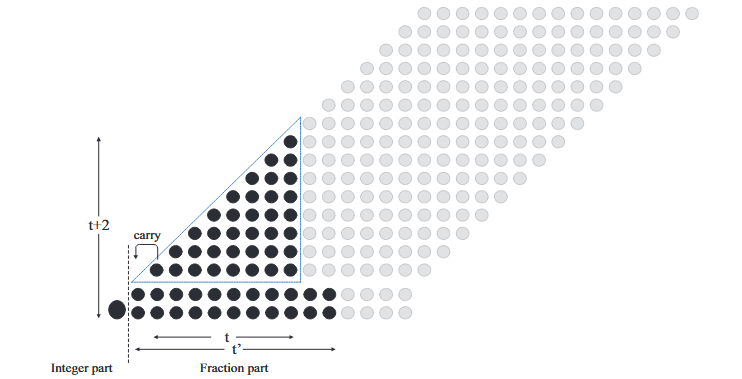
\includegraphics[width=0.8\textwidth]{dots}
\caption{点积图示意：LETAM中保留的部分积（黑色）与剪枝的部分积（灰色）}
\label{fig:dot_diagram}
\end{figure}

第一个关键模块是近似绝对值提取单元（Approximate Absolute Unit），用于在有符号场景下快速生成输入操作数的幅值。对于$n$位有符号输入$I$，其绝对值计算为
\begin{equation}
|I| =
\begin{cases}
I, & I[n-1] = 0 \\
\overline{I} + 1, & I[n-1] = 1
\end{cases}
\label{eq:abs_exact}
\end{equation}
原LETAM论文提出了一种局部增量近似绝对值方案，仅对低$z$位执行加一并将进位信号OR合并，以避免补码绝对值运算中的进位链延时。然而，该方案在8位配置下对某些负数（如$-32$的倍数）会产生恒定的绝对误差"1"。原论文指出该方案对大部分输入是精确的，最大相对误差发生在最小负数值上。本文选择标准补码绝对值$\overline{I}+1$，虽然增加了约$O(N)$的加法延迟，但彻底消除了该误差源。

第二个关键模块是前导一检测单元（Leading-One Detector），用于找出$|A|$与$|B|$的最高有效"1"位位置，并生成$k_A$、$k_B$。设$I$为输入幅值向量，前导一位置检测的逻辑形式为
\begin{equation}
k = \max\{i : I[i] = 1\}, \quad 0 \leq i \leq n-1
\label{eq:msof}
\end{equation}
对于零输入，$k$默认输出为0。该模块通过优先编码器从高位向低位扫描实现，其输出同时用于后续截断与移位重构。

第三个关键模块是截断单元（Truncation Unit），它依据前导位位置对幅值执行归一化截断操作。设移位量为
\begin{equation}
\mathrm{shift} = (N-1) - k
\end{equation}
截断过程可表示为
\begin{equation}
\mathrm{tmp} = I \ll \mathrm{shift}, \quad X^{t'} = \mathrm{tmp}[N+TP-1 : N]
\label{eq:truncate}
\end{equation}
即先将输入左移$\mathrm{shift}$位使最高有效位移至次高位，随后从移位结果的高位截取$TP$位作为归一化尾数$X^{t'}$。同时检测被丢弃的低$N$位是否存在非零比特（粘着位sticky bit）：
\begin{equation}
\mathrm{sticky} = \bigvee_{j=0}^{N-1} \mathrm{tmp}[j], \quad \text{if } \mathrm{shift} > 0
\label{eq:sticky}
\end{equation}
若粘着位为1，则将尾数LSB置1以进行舍入补偿。这一操作的硬件含义是：通过左移对齐后截取高位，避免了显式除法运算；粘着位检测覆盖被丢弃的全部$N$位而非固定位置的若干比特，确保了截断操作的统计无偏性——对于均匀分布的随机输入，粘着位为1的概率约为50\%，等效于就近舍入（round-to-nearest）的效果。从$TP$位尾数中进一步提取低$T$位供近似乘法核使用：$X^t = X^{t'}[TP-1 : TP-T]$。

第四个关键模块是近似乘法核（Arithmetic Block），完成式\eqref{eq:letam}中括号部分的计算。设$\mathrm{SUMW} = TP + T + 1$为内部求和位宽，$\mathrm{PRODW} = 2 \cdot TP$为全精度尾数乘积位宽，则计算流程如下：

\textbf{(1) 基底计算}：全精度尾数乘积$\mathrm{prod\_full} = X_A^{t'} \times X_B^{t'}$（$2 \cdot TP$位），截取高$\mathrm{SUMW}$位作为初始基底：
\begin{equation}
\mathrm{base} = \mathrm{prod\_full}[\mathrm{PRODW}-1 : \mathrm{PRODW}-\mathrm{SUMW}]
\label{eq:am_base}
\end{equation}
本文采用全精度尾数乘积作为初始基底，这是本文提出的一项改进，使得基底本身即为精确的部分积之和，后续的$\beta$补偿项仅需修正因低位截断引入的残差，从而显著降低了补偿系数的敏感度，提高了设计的鲁棒性。

\textbf{(2) 线性补偿}：计算低位截断尾数之和$\mathrm{lower\_sum} = X_A^t + X_B^t$（带符号扩展至$T+1$位），叠加补偿项：
\begin{equation}
\mathrm{corr} = \frac{\mathrm{lower\_sum} \cdot \beta_{\mathrm{num}}}{\beta_{\mathrm{den}}}
\label{eq:am_corr}
\end{equation}
典型参数配置为$\beta = 3/8$。该补偿项修正了因低位截断引入的线性偏差，其硬件实现仅需一次加法与一次常数乘除法。

\textbf{(3) 非线性校正}：对$T$位尾数的截断乘积进行缩放校正：
\begin{equation}
\mathrm{scale\_corr} = \frac{\mathrm{trunc}(X_A^t \times X_B^t) \cdot \alpha_{\mathrm{num}}}{\alpha_{\mathrm{den}}}
\label{eq:am_scale}
\end{equation}
其中$\mathrm{trunc}(\cdot)$表示对$T \times T$位完整乘积右移$T-1$位后保留$T+1$位，典型参数$\alpha = 1/16$。该校正项进一步修正大数值区域的误差分布。最终输出定点和为
\begin{equation}
\mathrm{sum\_fixed} = \mathrm{base} + \mathrm{corr} + \mathrm{scale\_corr}
\label{eq:am_sum}
\end{equation}

第五个关键模块是移位重构单元（Shift Unit），根据指数重建偏移量对AM\_block输出的定点和执行移位操作以恢复最终乘积的量级。移位量的计算公式为
\begin{equation}
\mathrm{shift\_amt} = k_A + k_B + 2 - \mathrm{SUMW}
\label{eq:shift_amt}
\end{equation}
其中常数偏移量$+2$用于对齐AM\_block内部定点小数点位置，$-\mathrm{SUMW}$将尾数乘积的隐含指数归一化至整数域。移位方向由$\mathrm{shift\_amt}$的正负决定：正值左移（放大），负值右移（缩小），溢出时自动饱和截断。

为进一步提升精度，引入自适应增益补偿机制。根据两操作数的同异号属性以及前导一索引之和$k_{\mathrm{sum}} = k_A + k_B$的量级，动态选择增益倍数$G(k_{\mathrm{sum}}, s)$：
\begin{equation}
G(k_{\mathrm{sum}}, s) =
\begin{cases}
10/8 = 1.25, & s = 1,\ k_{\mathrm{sum}} \geq 12 \\
9/8 = 1.125, & s = 1,\ 8 \leq k_{\mathrm{sum}} < 12 \\
8/8 = 1.000, & s = 1,\ k_{\mathrm{sum}} < 8 \\
7/8 = 0.875, & s = 0,\ k_{\mathrm{sum}} \geq 10 \\
8/8 = 1.000, & s = 0,\ k_{\mathrm{sum}} < 10
\end{cases}
\label{eq:gain}
\end{equation}
其中$s=1$表示同号，$s=0$表示异号。增益采用整数运算实现：$\mathrm{out}_{\mathrm{gain}} = (\mathrm{in} \times G_{\mathrm{num}}) / G_{\mathrm{den}}$，且仅在补偿后结果大于原始值时生效（仅向上修正），避免过补偿导致的精度退化。对于极小幅值输入（$|A|<8$或$|B|<8$），自动旁路近似通路直接输出精确乘积，消除零区域附近的系统性偏差。最后，符号恢复逻辑根据$A[n-1] \oplus B[n-1]$对幅值乘积执行补码取反操作，得到最终的有符号输出。


\clearpage

\section{近似乘法器的RTL设计与验证分析}

基于前文对近似乘法器架构的分析，本节将详细阐述所选用近似乘法器 IP 的 RTL 实现流程、
模块划分方案、核心创新点，以及算子级与应用级的误差分析和精度验证方法。
通过系统化的设计与验证流程，保障所实现的近似乘法器在实现预期 PPA 优化目标的同时，
能够在实际应用场景中维持可接受的计算精度。需要说明的是，本文所复现的近似
乘法器均为有符号8bit乘法器，后续
将重点对量化至8bit版本的近似乘法器进行性能与精度验证，确保其适配目标应用场景的量化需求。


\subsection{近似乘法器的底层RTL设计}

为兼顾参数化开发效率与工程级集成，本研究采用基于 Scala 的 Chisel 作为算子级 
RTL 开发语言。Chisel 在抽象表达、参数化生成及与 Chipyard 
等开源生态的兼容性方面具备较好的适配性，便于在不同参数配置间
快速迭代电路结构并保持代码可复用性。基于此，本文构建了从 Chisel 源
码到门级网表的标准化复现流程（见图~\ref{fig:chisel-flow}）：首
先在 Chisel 层实现参数化算子并完成单元测试；其次通过编译链生
成符合工程规范的 SystemVerilog RTL；最后以该 RTL 为对象开展功能一致性仿真、门
级时序验证与 EDA 前端的逻辑综合评估。该流程既保证了设计的工程可验证性，
也为后续系统级集成和 PPA 评估提供了可重复的实现路径。

\begin{figure}[htbp]
    \centering
    \begin{tikzpicture}[
        node distance=1.2cm,
        block/.style={rectangle, draw=black!80, thick, fill=black!3, text width=2.6cm, align=center, rounded corners=2pt, minimum height=1.4cm, font=\small},
        line/.style={draw=black!80, thick, -{Stealth[length=2.5mm, width=1.5mm]}, shorten >=1pt, shorten <=1pt}
    ]
        \node [block] (chisel) {Chisel\\参数化源代码};
        \node [block, right=of chisel] (sv) {SystemVerilog\\RTL代码生成};
        \node [block, right=of sv] (sim) {标准仿真器\\功能验证};
        \node [block, right=of sim] (synth) {EDA工具链\\逻辑综合评估};

        \draw[line] (chisel) -- node[midway, above=3pt, font=\scriptsize] {编译} (sv);
        \draw[line] (sv) -- (sim);
        \draw[line] (sim) -- (synth);
    \end{tikzpicture}
    \caption{基于 Chisel 的近似算子底层设计与复现流程范式}
    \label{fig:chisel-flow}
\end{figure}

\subsubsection{TOSAM近似乘法器的RTL实现}

本文对 TOSAM 的 RTL 复现采用 Chisel 参数化建模方法，将算法参数、模块边界与位宽推导统一收敛到生成器框架中。工程首先在 \texttt{TOSAMConfig} 中定义输入位宽 $n$、舍入参数 $h$ 与符号属性，并自动派生截断参数 $t$、小乘法器位宽以及分数和位宽
\(
l=2+\max(t,2h+2)
\)。
这种实现方式使前文的近似乘积表达式能够直接映射为结构参数，而无需在不同模块中重复维护常量。随后，\texttt{TOSAMGenerator} 根据命令行参数或环境变量实例化 \texttt{TOSAM} 或 \texttt{TOSAMSigned}，并调用 CIRCT 后端生成 SystemVerilog；面向 Gemmini 集成时，则进一步通过 \texttt{ApproxMulGenerator} 固定导出 8 位有符号输入、16 位有符号输出的 \texttt{approx\_mul\_single.sv}，从而得到可以直接嵌入处理单元的数据通路实现。代码~\ref{lst:tosam-config} 给出了参数配置与顶层实例化的基本形式。

\begin{lstlisting}[caption={TOSAM 的参数化配置与顶层实例化方式},label={lst:tosam-config},basicstyle=\ttfamily\small]
case class TOSAMConfig(n: Int = 16, h: Int = 3, signed: Boolean = true) {
  val t: Int = if (h > 0) h + 4 else 3
  val smallMultWidth: Int = h + 1
  val fracSumWidth: Int = 2 + math.max(t, 2 * h + 2)
  val outputWidth: Int = 2 * n
}

val config = TOSAMConfig(n = 8, h = 3, signed = true)
val multiplier = Module(new TOSAMSigned(config))
\end{lstlisting}

对于无符号主路径，\texttt{TOSAM.scala} 严格对应式~\eqref{eq:tosam_final} 的硬件分解过程。首先，两个 \texttt{LeadingOneDetector} 分别提取输入最高有效位位置，并利用 \texttt{found} 信号完成零输入检测。随后，\texttt{TruncationUnit} 通过
\(
\texttt{io.in << ((n-1)-k)}
\)
完成标准化左移，再直接截取高位分数部分，得到 $(Y_A)_t$ 与 $(Y_B)_t$。第三步的 \texttt{ArithmeticUnit} 是近似核的核心：\texttt{RoundingUnit} 仅保留截断结果的前 $h$ 位并在最低位补入常数 1，以实现 odd-rounding；\texttt{SmallMultiplier} 对两个 $(h+1)$ 位近似分数执行精确乘法；随后算术核心根据 $t$ 与 $2h+2$ 的大小关系完成位宽对齐，并与常数项及两个截断项相加。最后，\texttt{ShiftUnit} 以 $\max(t,2h+2)$ 为偏移基准，在 \texttt{kA + kB} 大于该偏移时执行左移，否则执行右移，从而恢复指数部分的量级。整个主路径保持为纯组合结构，有利于后续综合与关键路径分析。代码~\ref{lst:tosam-arith} 给出了算术核心中最关键的组合逻辑。

\begin{lstlisting}[caption={ArithmeticUnit 的关键组合逻辑},label={lst:tosam-arith},basicstyle=\ttfamily\small]
val roundA = Module(new RoundingUnit(t, h))
val roundB = Module(new RoundingUnit(t, h))
val mult = Module(new SmallMultiplier(h + 1))

if (t > 2 * h + 2) {
  val one = Cat(1.U(2.W), 0.U(t.W))
  val paddedMult = Cat(mult.io.product, 0.U((t - 2 * (h + 1)).W))
  io.result := one +& io.yAt +& io.yBt +& paddedMult
} else {
  val alignWidth = 2 * h + 2
  val one = Cat(1.U(2.W), 0.U(alignWidth.W))
  io.result := one +& paddedYAt +& paddedYBt +& mult.io.product
}
\end{lstlisting}

在有符号实现中，\texttt{TOSAMSigned.scala} 并未直接构造补码近似乘法器，而是采用“幅值变换、无符号近似乘法、符号恢复”的分层封装策略。两个 \texttt{ApproxAbs} 模块首先输出输入操作数的幅值与符号位，其中对最小负数采用饱和到最大正值的处理，以避免补码绝对值运算中的溢出问题；随后调用无符号 \texttt{TOSAM} 完成近似乘法，再通过异或得到结果符号，并在输出端进行一次范围裁剪。该实现既保持了无符号近似核的可复用性，也降低了有符号版本的额外设计复杂度。

由 \texttt{ApproxMulGenerator} 导出的 \texttt{approx\_mul\_single.sv} 已经被整理为单文件
 SystemVerilog，其内部依次包含 \texttt{ApproxAbs}、\texttt{LeadingOneDetector}、
 \texttt{TruncationUnit}、\texttt{RoundingUnit}、\texttt{SmallMultiplier}、
 \texttt{ArithmeticUnit}、\texttt{ShiftUnit}、\texttt{TOSAM}、\texttt{TOSAMSigned} 
 与 \texttt{approx\_mul} 十个模块。与 Chisel 源码相比，生成后的 RTL 不再保留参数推导，
 而是展开为固定 8 位配置下的静态组合逻辑。

\subsubsection{ZBA-BM近似乘法器的RTL实现}
\label{subsec:zbabm-rtl}

本文对 ZBA-BM 的 RTL 实现同样采用 Chisel 参数化建模，将式~\eqref{eq:zbabm_pp} 给出的部分积单解析式与 Row-0 选择性部分积补偿映射为可直接综合的组合电路，再经 Chisel 编译流程导出为 SystemVerilog 供后端综合。本节按部分积阵列生成、Row-0 PPSC 落地、$N/2+1$ 行稀疏外挂、与 Gemmini PE 集成四部分给出核心结构。

模块顶层为 8~bit 有符号输入与 16~bit 有符号输出的纯组合逻辑，不引入寄存器或时钟域，可在 PE 数据流的任一时序级直接接入而无时序握手开销：

\begin{lstlisting}[caption={ZBA-BM 顶层 Chisel 接口},label={lst:zbabm-iface},basicstyle=\ttfamily\small,language={}]
class ZBABM_PPSC extends Module {
  val io = IO(new Bundle {
    val a = Input(UInt(8.W))
    val b = Input(UInt(8.W))
    val product = Output(SInt(16.W))
  })}
\end{lstlisting}

扩展乘数 $b_{\text{ext}} = \mathtt{Cat(b,\;0.U(1.W))}$，
4 行部分积以 \texttt{Vec(4, UInt(16.W))} 在循环中展开。
每行从 $b_{\text{ext}}$ 取 3 位窗口 $B_W^{(i)}$，
直接由窗口高位解出极性标志 $\mathtt{neg} = b_{2i+1}$，
由窗口三位的同向比较解出零标志 $\mathtt{zero} = (B_W = \mathtt{000} \lor B_W = \mathtt{111})$。
随后按式~\eqref{eq:zbabm_pp} 在 9 个部分积位 $j$ 上以位运算实现单解析式：

\begin{lstlisting}[caption={K-Map 单比特部分积的 Chisel 实现},label={lst:zbabm-pp-chisel},basicstyle=\ttfamily\small,language={}]
val approx_bit = (!zero) & (a_bit ^ neg)
pp_bits(j) := approx_bit
\end{lstlisting}

在 $i = 0$ 时，
模块进入第二条分支：先生成与其他行相同的 \texttt{approx\_bit}，
再以同一 K-Map 单解析式套用 $a_{j-1}$ 替代 $a_j$ 作为输入，得到精确 $-2A$ 分支 \texttt{exact\_bit}，
通过 \texttt{Mux(is\_100, exact\_bit, approx\_bit)} 实现式~\eqref{eq:zbabm_ppsc} 的局部补偿支路。
RTL 保留通用 K-Map 结构而仅替换 $a$ 信号源，
在 $B_W = \mathtt{100}$ 下 $\mathtt{neg}=1$、$\mathtt{zero}=0$，化简后等价于式~\eqref{eq:zbabm_ppsc} 的 $pp_j = a_{j-1}$：

\begin{lstlisting}[caption={Row-0 PPSC 的 Chisel 实现},label={lst:zbabm-ppsc-chisel},basicstyle=\ttfamily\small,language={}]
val is_100 = b_bits === 4.U
val a_bit_2 = if (j == 0) false.B else io.a(j-1)
val approx_bit = (!zero) & (a_bit ^ neg)
val exact_bit  = (!zero) & (a_bit_2 ^ neg)
pp_bits(j) := Mux(is_100, exact_bit, approx_bit)
\end{lstlisting}

4 行部分积按 $\ll 2i$ 对齐拼接为 \texttt{rows(0..3)}。
负向符号扩展位 $\mathtt{neg\_bits}_i$ 不并入主部分积阵列，
而以稀疏第 5 操作数的形式与四行并列：

\begin{lstlisting}[caption={稀疏第 5 操作数的并行累加},label={lst:zbabm-reduce},basicstyle=\ttfamily\small,language={}]
val operands = Seq(
  rows(0), rows(1), rows(2), rows(3),
  neg_bits(0).asUInt,
  neg_bits(1).asUInt << 2,
  neg_bits(2).asUInt << 4,
  neg_bits(3).asUInt << 6)
val sum = operands.reduce(_ + _)
io.product := sum.asSInt
\end{lstlisting}

Chisel 编译后端将该 \texttt{reduce} 表达式展开为扁平加法树，由综合工具自动调度内部 3:2 压缩器，使 Fmax 不被 $N/2+1$ 外挂行主导，相关实证见 §\ref{subsec:ppa}。

PE 内的近似 MAC 单元直接以 Chisel 模块形式实例化 ZBA-BM，不引入外部 SystemVerilog 黑盒模块：

\begin{lstlisting}[caption={ZBA-BM 在 Gemmini PE 中的集成},label={lst:zbabm-pe},basicstyle=\ttfamily\small,language={}]
val zbabm = Module(new ZBABM_PPSC())
zbabm.io.a := io.in_a.asTypeOf(UInt(8.W))
zbabm.io.b := io.in_b.asTypeOf(UInt(8.W))
val approx_math = zbabm.io.product
val product = Mux(io.approx_level > 0.U, approx_math, exact_math)
\end{lstlisting}

精确通路 \texttt{exact\_math} 保留，PE 通过 RoCC 指令的 \texttt{approx\_level} 控制位在精确与近似之间切换。这一并列结构使后续系统级仿真中 ZBA-BM 与精确实现的输出差异严格归因于乘法器本身。

\subsubsection{LETAM 乘法器的 RTL 实现}

本文对 LETAM 近似乘法器的 RTL 实现采用参数化构型，将截断参数 $T$（乘法项保留位宽）、$TP$（加法项保留位宽）与零偏阈值 $Z$ 统一映射至顶层生成框架。该实现规避了多模块间的常量重复定义，使代码层级直接对应于式\eqref{eq:letam}定义的补偿策略与截断流程。其中，针对基准推荐配置 LETAM(3,6)（即 $N=8, T=3, TP=6, Z=5$），内部定点求和位宽参数 $\mathrm{SUMW}$ 自动演化为 $TP+T+1$，从而完全控制核心乘积运算结构的数据流带宽。

数据通路被划分为绝对值提取、前导一检测与截去、近似乘法核运算、移位重构以及后处理增益补偿五大计算流水簇，支持在一个时钟周期内无缝走完全部组合逻辑。

首先，预处理阶段负责对于输入操作数 $A$ 与 $B$ 完成至无符号幅值域 $|A|$ 与 $|B|$ 的映射，同时旁路析出两端符号位 $s_A$ 与 $s_B$ 用于末级的极性恢复。

随后，电路进入前导一检测与粘着位截断（MSOF）阶段。该部分使用优先级编码结构对 $|A|$ 与 $|B|$ 实施前导一检测（MSB-1），获取位级索引 $k_A$ 与 $k_B$。接着依据左移归一化量 $\mathrm{shift} = (N-1) - k$ 将数据上调至满幅，截取高 $TP$ 位获得主尾数 $X^{t'}$。同时，为了减轻极低位舍入带来的系统性欠估计，运算流水提取出被抛弃的低 $N$ 位构成粘着位（Sticky Bit）。若存在截留非零量，则使 $X^{t'}$ 最低位置 1 进行进位补充，并分理出 $T$ 位特征辅助尾数 $X^t$ 供后续补偿使用。

在获取主尾数与特征尾数后，近似核心运算单元（AM\_block）在求和位宽 $\mathrm{SUMW}$ 内完成对尾数乘积的重构。其核心映射逻辑如下：

\begin{lstlisting}[caption={LETAM AM\_block 补偿校正的 Verilog 实现},label={lst:letam-am-block},basicstyle=\ttfamily\small,language={}]
// 1) 基础无符号基底截取
assign base = prod_full[PRODW-1 : PRODW-SUMW];
// 2) 线性位移补偿 (超参数 \beta)
assign corr = (lower_sum * BETA_NUM) / BETA_DEN;
// 3) 交叉非线性校正 (超参数 \alpha)
assign scale_corr = (trunc_cross * ALPHA_NUM) / ALPHA_DEN;
// 输出定点和
assign sum_fixed = base + corr + scale_corr;
\end{lstlisting}

基础基底 \texttt{base} 来源于 $X_A^{t'} \times X_B^{t'}$ 的高向截位，其保留位宽限定在 $\mathrm{SUMW}$ 边界。由分段衰减产生的线性误差通过 $\mathrm{lower\_sum} = X_A^t + X_B^t$ 借助常量 $\beta$（取 $3/8$）施加一次位移推移修正；非线性效应部分依靠截断后的交叉乘积借助常量 $\alpha$（取 $1/16$）展开二次逼近修正。硬件系统通过构建底层的定点加法树拼接上述偏置项，有效压缩了双通路精确相乘的高昂建树成本。

最后，系统需完成位阶重建与自适应增益修正。取得上述的定点拼接结果后，根据式\eqref{eq:shift_amt}提供的位级移动参考量 $\mathrm{shift\_amt}$ 执行双端饱和范围受限的对数反映射移位。针对小数值域在对数域处理引起的深陷发散现象，电路基于索引累加量 $k_A+k_B$ 计算非线性增益补偿因子 $G$ 对结果进行牵引放缩。其中特别设置了极值门限旁路判定：当探测到输入处于 $|A|,|B| < Z$ （推荐阈值 $Z=5$）地带时，主补偿回路直接休眠，由精确通路接管输出以避免深渊处的百分比偏差放大。综合完所有运算后，合并原始的 $s_A \oplus s_B$ 特征并在输出端最终翻转为完整的 16 位有符号乘积。

\subsection{算子级全遍历误差分析}
为了全面评估近似乘法器的误差特性，本研究采用全遍历仿真方法，
对每一个输入组合计算精确乘积与近似乘积之间的误差，并统计误差分布、
平均误差、最大误差等关键指标。通过分析这些统计结果，可以深入理解近似乘
法器在不同输入条件下的表现，为后续的应用级精度验证提供理论基础。

本文采用以下标准误差指标对近似乘法器进行量化评估。设$P_i$为第$i$组输入的精确乘积，
$P_{i,\mathrm{app}}$为近似乘积，$N$为样本总数，$P_{\max}$为精确乘积的最大幅值，则各指标定义如下：

\begin{table}[H]
\centering
\caption{误差评估指标定义}
\label{tab:error_metrics_def}
\begin{tabular}{lll}
\toprule
\textbf{指标} & \textbf{全称} & \textbf{定义} \\
\midrule
ME & Mean Error & $\frac{1}{N}\sum (P_i - P_{i,\mathrm{app}})$ \\
MAE & Mean Absolute Error & $\frac{1}{N}\sum |P_i - P_{i,\mathrm{app}}|$ \\
RMSE & Root Mean Square Error & $\sqrt{\frac{1}{N}\sum(P_i - P_{i,\mathrm{app}})^2}$ \\
MARE & Mean Absolute Relative Error & $\frac{100}{N}\sum \left|\frac{P_i - P_{i,\mathrm{app}}}{P_i}\right| (\%)$ \\
MRED & Mean Relative Error Distance & $\frac{100}{N}\sum \frac{|P_i - P_{i,\mathrm{app}}|}{|P_i| + |P_{i,\mathrm{app}}|} (\%)$ \\
NMED & Normalized Mean Error Distance & $\frac{\mathrm{MAE}}{|P_{\max}|} \times 10^3$ \\
\bottomrule
\end{tabular}
\end{table}

\subsubsection{TOSAM误差分析}

针对 TOSAM 的算子级误差特性，本文对四组配置 TOSAM$(0,3)$、TOSAM$(1,4)$、TOSAM$(2,6)$ 
与 TOSAM$(3,7)$ 分别进行了 8 位有符号乘法全遍历分析。输入覆盖区间为 $[-128,127]$，共得到 $65\,536$ 组样本；对每组样本同时计算精确乘积与近似乘积，并以
\(
e_{\mathrm{raw}}=P_{\mathrm{apx}}-P_{\mathrm{exact}}
\)
为基础统计 MAE、RMSE、相对误差、最坏误差及误差分位点，同时结合误差直方图、
输入空间热力图和箱线图观察误差在全输入域内的分布特征。

表~\ref{tab:tosam-error-compare} 给出了四组配置的统一统计结果。可以看出，随着参数 $h,t$ 增大，误差指标呈现出明显的单调下降趋势：MAE 由 TOSAM$(0,3)$ 的 $339.18$ 下降至 TOSAM$(3,7)$ 的 $45.42$，RMSE 由 $598.58$ 下降至 $72.90$，P99 原始误差也由 $2046$ 收缩至 $224$。与此同时，所有配置的中位误差均为 0，且未出现符号翻转错误，说明 TOSAM 的主要问题并非符号失真，而是低精度配置下截断误差和尾部误差过大。对于矩阵乘法这类累加深度较高的场景，TOSAM$(0,3)$、TOSAM$(1,4)$ 和 TOSAM$(2,6)$ 的最坏误差与高分位误差仍然偏大，经过多次乘加累积后容易放大为不可忽略的输出偏差，因此难以满足后续系统级应用对误差传播的约束。

\begin{table}[htbp]
    \centering
    \caption{四组 TOSAM 配置的全遍历误差统计对比}
    \label{tab:tosam-error-compare}
    \small
    \setlength{\tabcolsep}{5pt}
    \begin{tabular}{lcccc}
        \toprule
        指标 & TOSAM$(0,3)$ & TOSAM$(1,4)$ & TOSAM$(2,6)$ & TOSAM$(3,7)$ \\
        \midrule
        ME & $-0.0625$ & $-0.0313$ & $-0.0166$ & $-0.0095$ \\
        MAE & $339.18$ & $168.90$ & $86.63$ & $45.42$ \\
        RMSE & $598.58$ & $277.15$ & $140.29$ & $72.90$ \\
        MARE & $7.91\%$ & $4.26\%$ & $2.24\%$ & $1.20\%$ \\
        WRE & $25.00\%$ & $13.89\%$ & $6.64\%$ & $3.81\%$ \\
        WAE & $4096$ & $2048$ & $1088$ & $624$ \\
        $P99_{\mathrm{raw}}$ & $2046$ & $845$ & $436.65$ & $224$ \\
        Sign Errors & $0$ & $0$ & $0$ & $0$ \\
        \bottomrule
    \end{tabular}
\end{table}

从图~\ref{fig:tosam-hist-grid}--图~\ref{fig:tosam-heat-grid} 也可以直观看到这一变化规律。
低精度配置的直方图具有更宽的尾部，热力图中高误差点在大幅值输入区域更加密集
；而 TOSAM$(3,7)$ 的误差分布已明显收敛，误差主体集中在零附近，
输入空间边缘的高误差区域亦得到有效压缩。结合 8 位乘法本身有效精度有限这一事实可以看出，
当可用位宽较小时，过于激进的截断会直接侵蚀有效数值信息，使局部乘法误差在乘加链中快速累积。
基于这一结果，本文后续系统集成与应用级验证仅保留 TOSAM$(3,7)$ 作为候选配置；
其余参数组合虽然具有更高的硬件节省潜力，但误差水平难以满足矩阵乘法累积误差控制的实际要求。

\begin{figure}[htbp]
    \centering
    \begin{subfigure}[b]{0.46\textwidth}
        \centering
        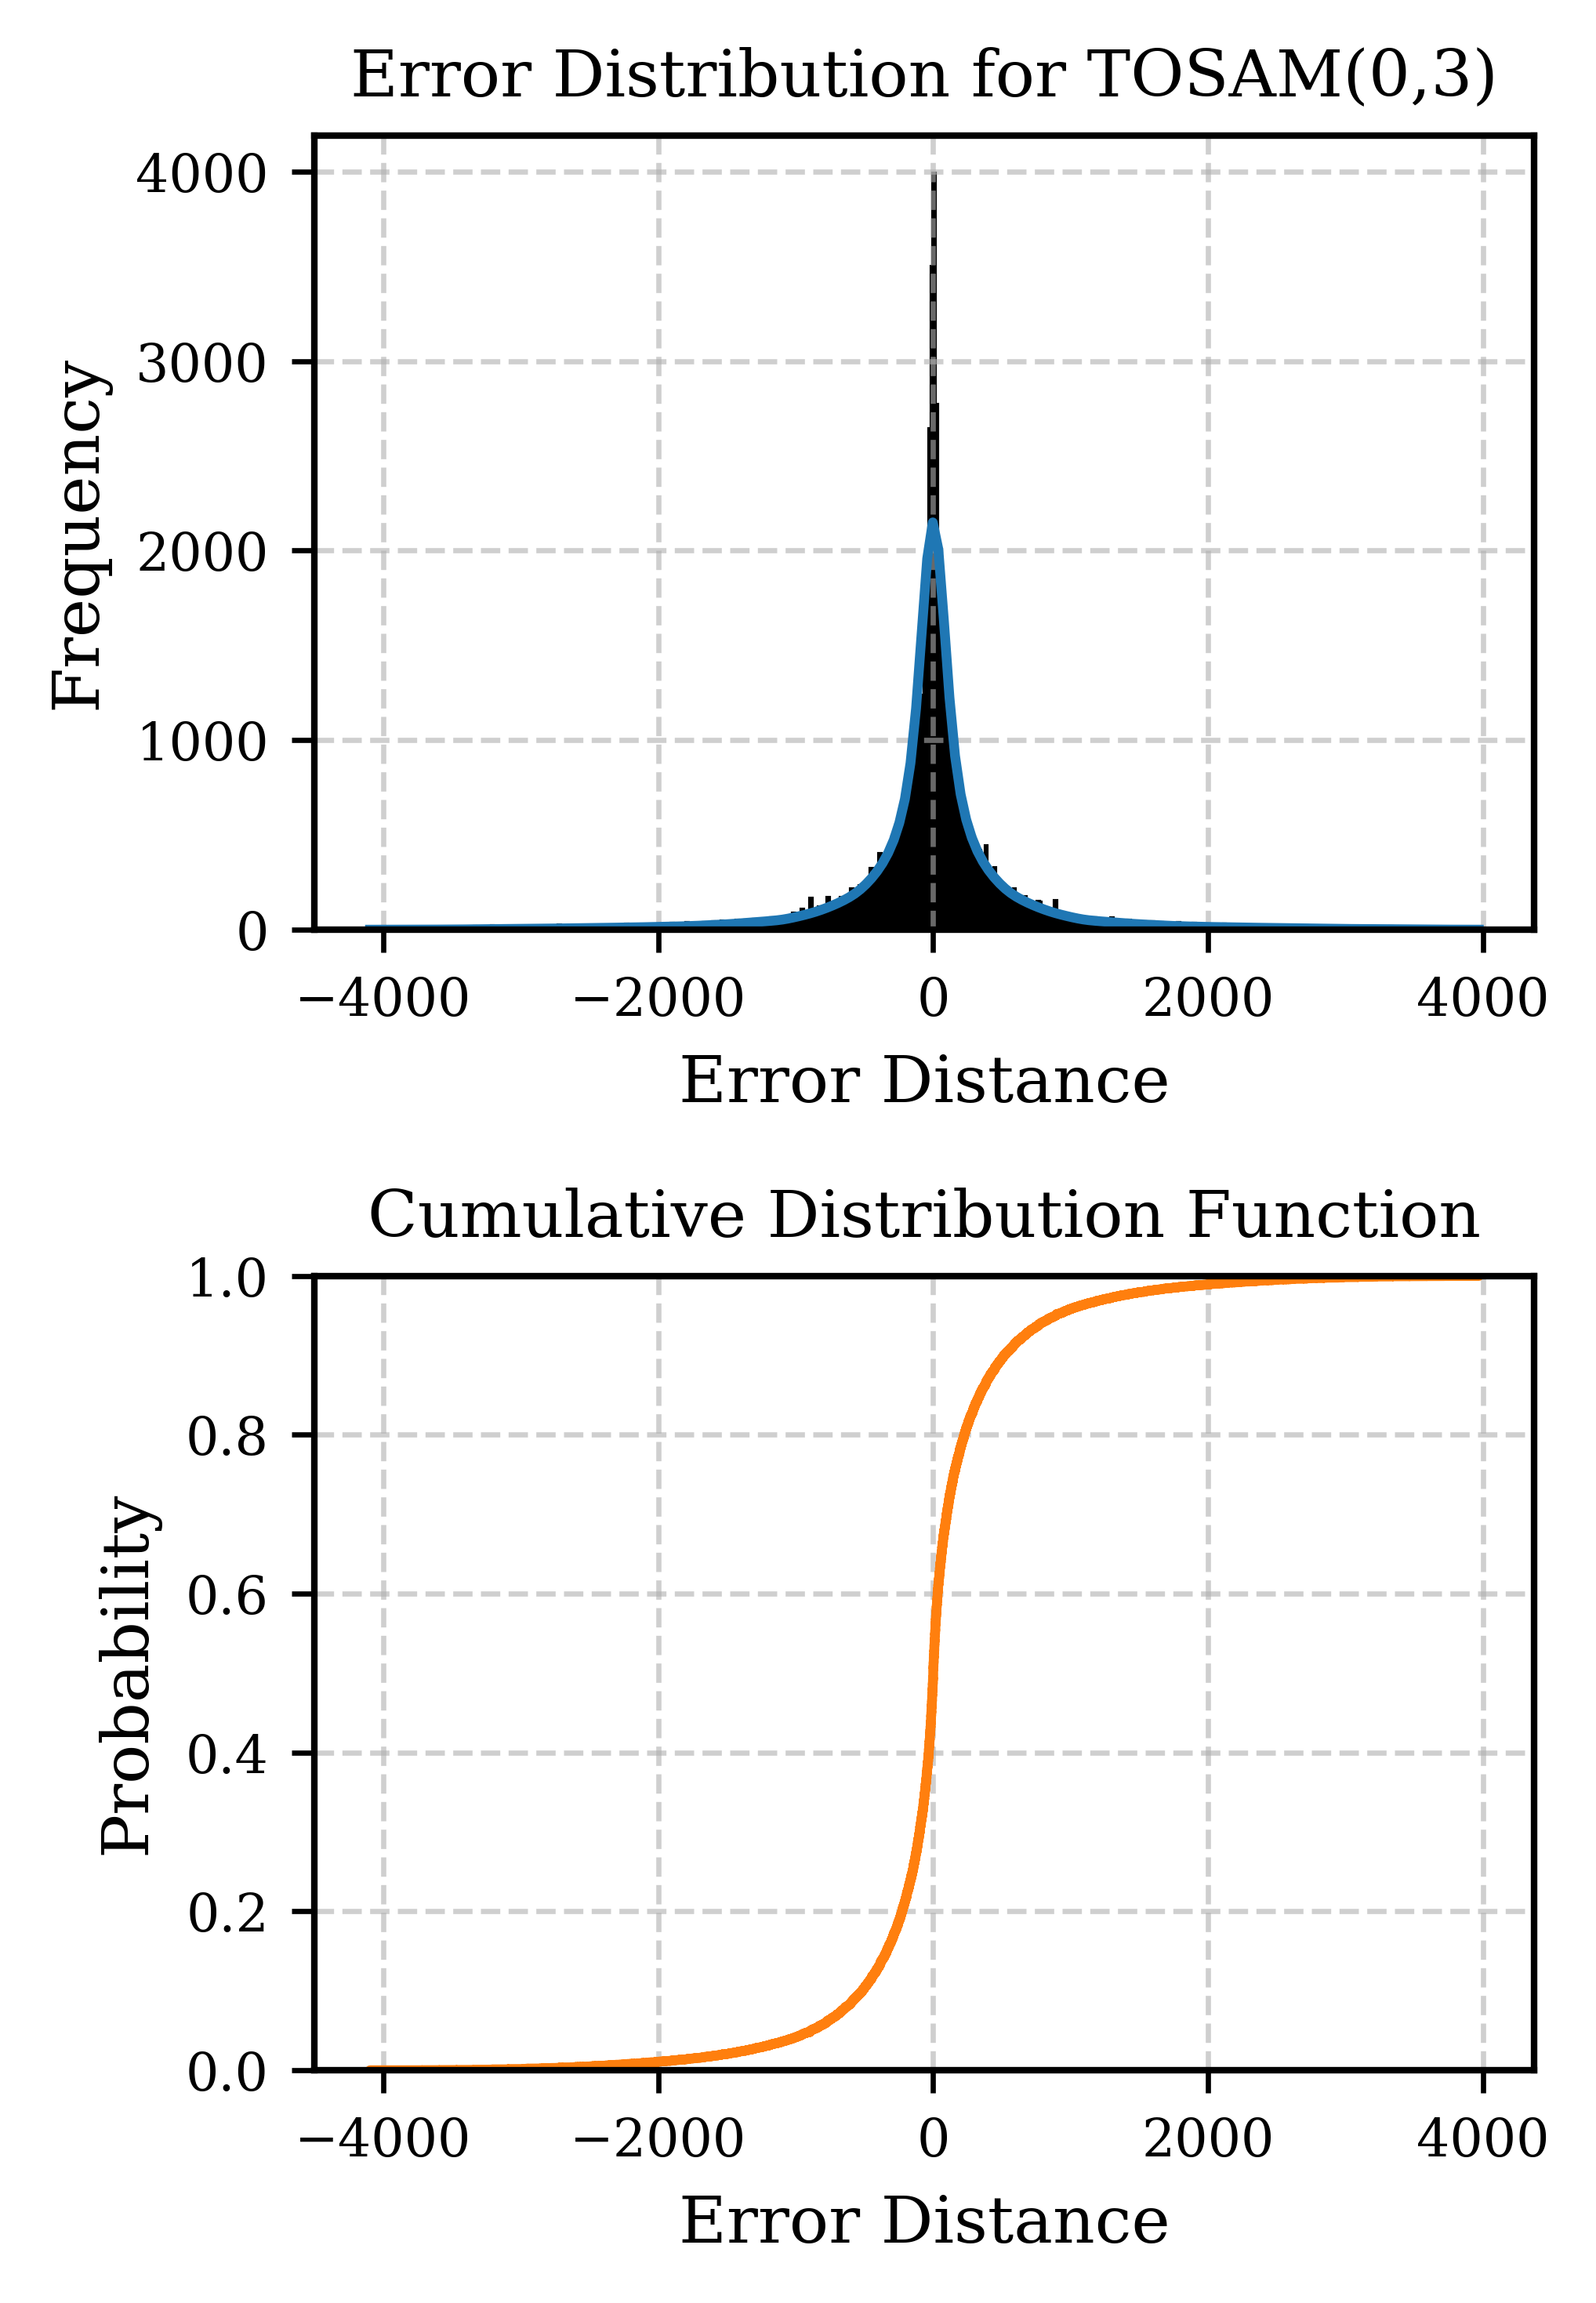
\includegraphics[width=\textwidth]{figures/08_tosam03_histogram.png}
        \caption{TOSAM$(0,3)$}
    \end{subfigure}\hfill
    \begin{subfigure}[b]{0.46\textwidth}
        \centering
        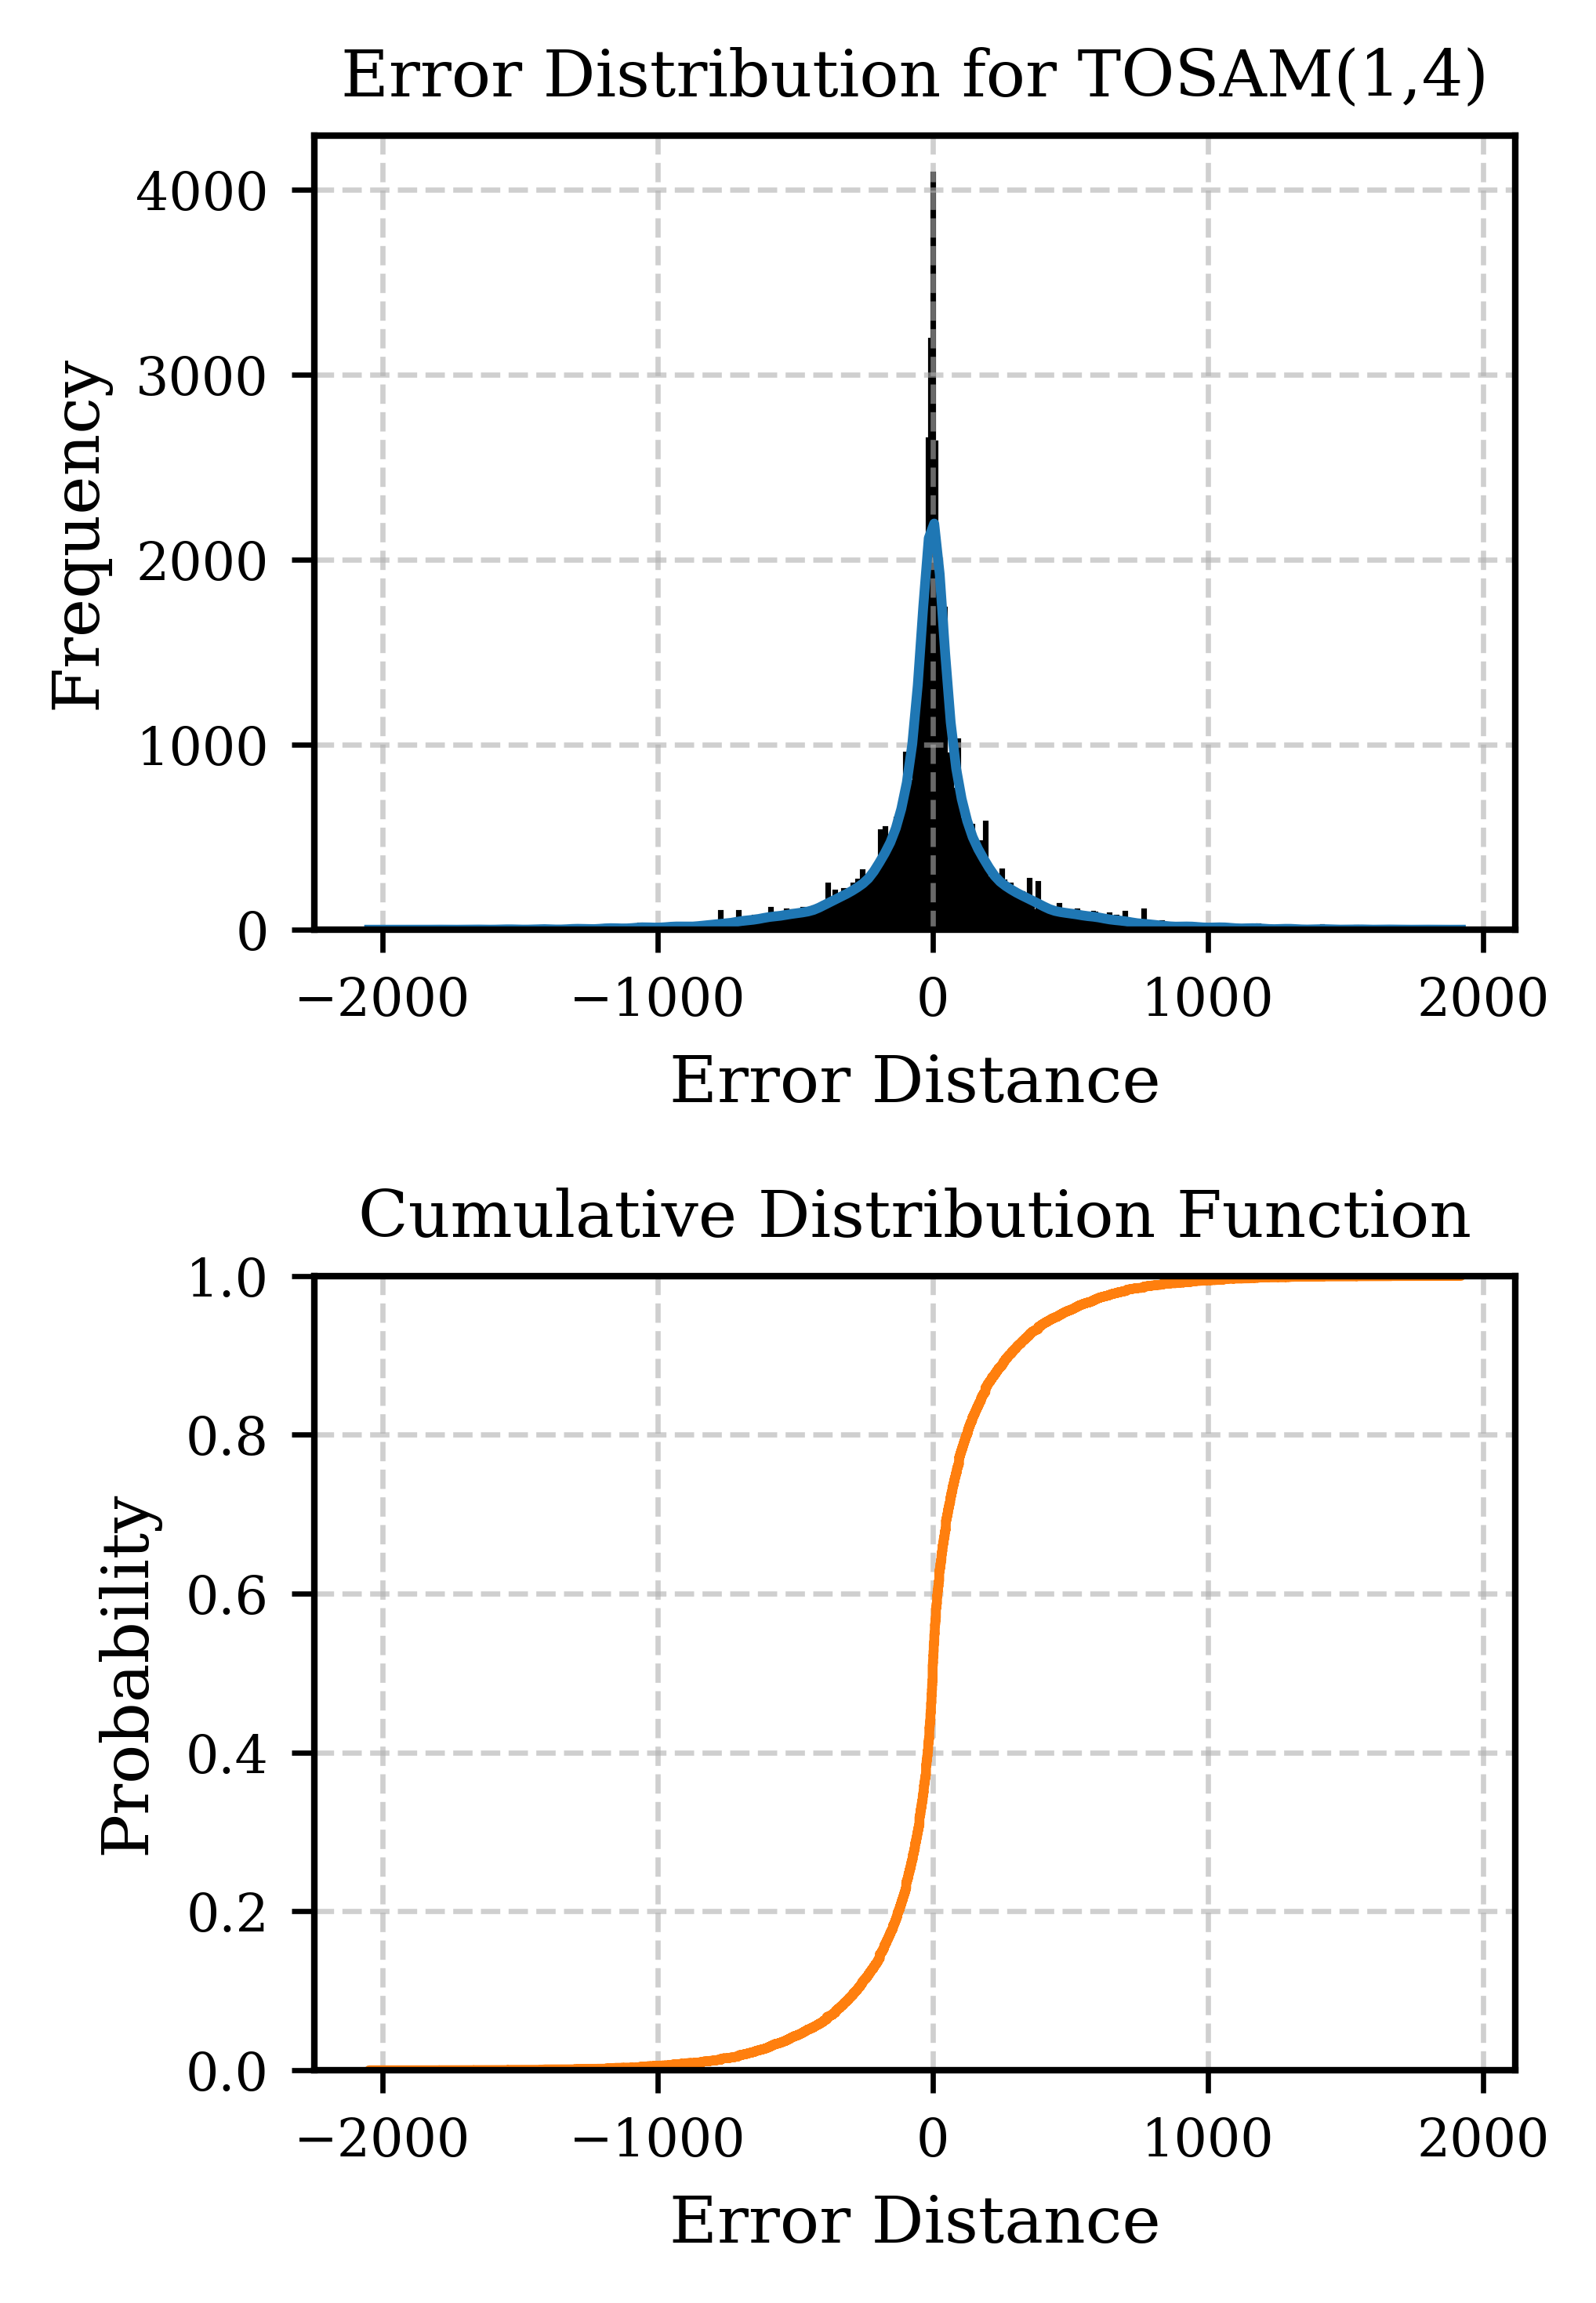
\includegraphics[width=\textwidth]{figures/08_tosam14_histogram.png}
        \caption{TOSAM$(1,4)$}
    \end{subfigure}

    \vspace{0.2em}

    \begin{subfigure}[b]{0.46\textwidth}
        \centering
        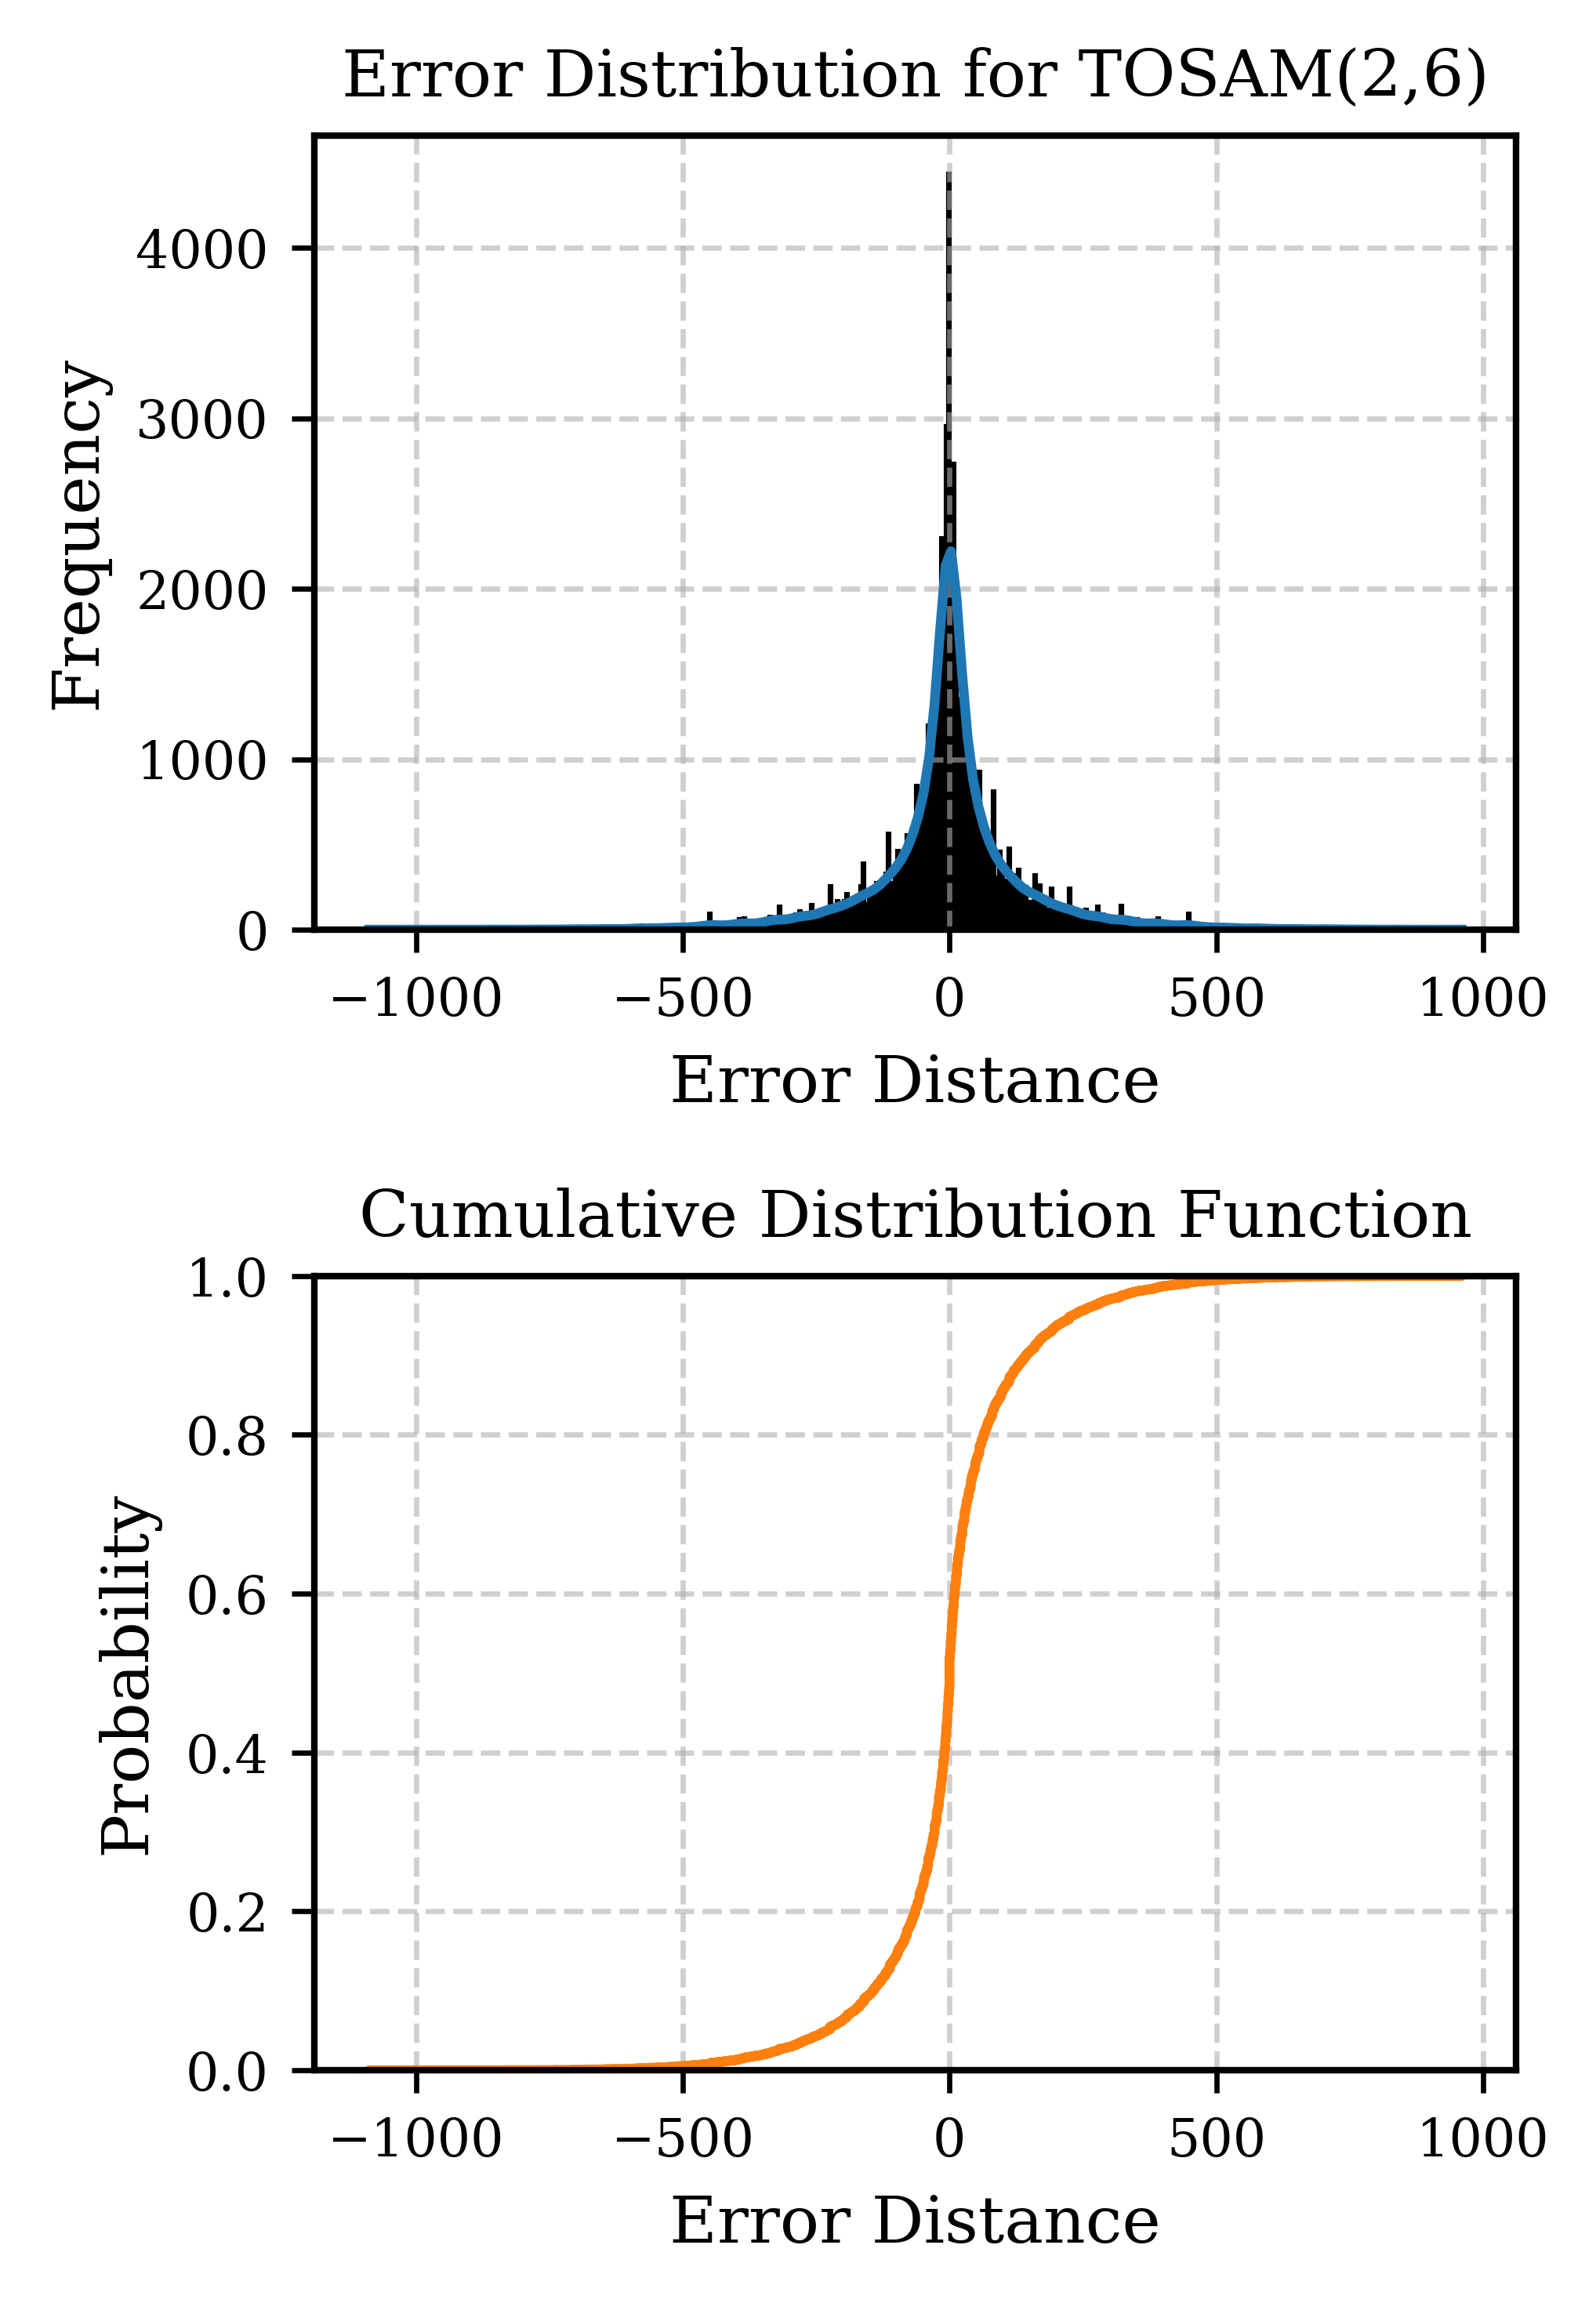
\includegraphics[width=\textwidth]{figures/08_tosam26_histogram.png}
        \caption{TOSAM$(2,6)$}
    \end{subfigure}\hfill
    \begin{subfigure}[b]{0.46\textwidth}
        \centering
        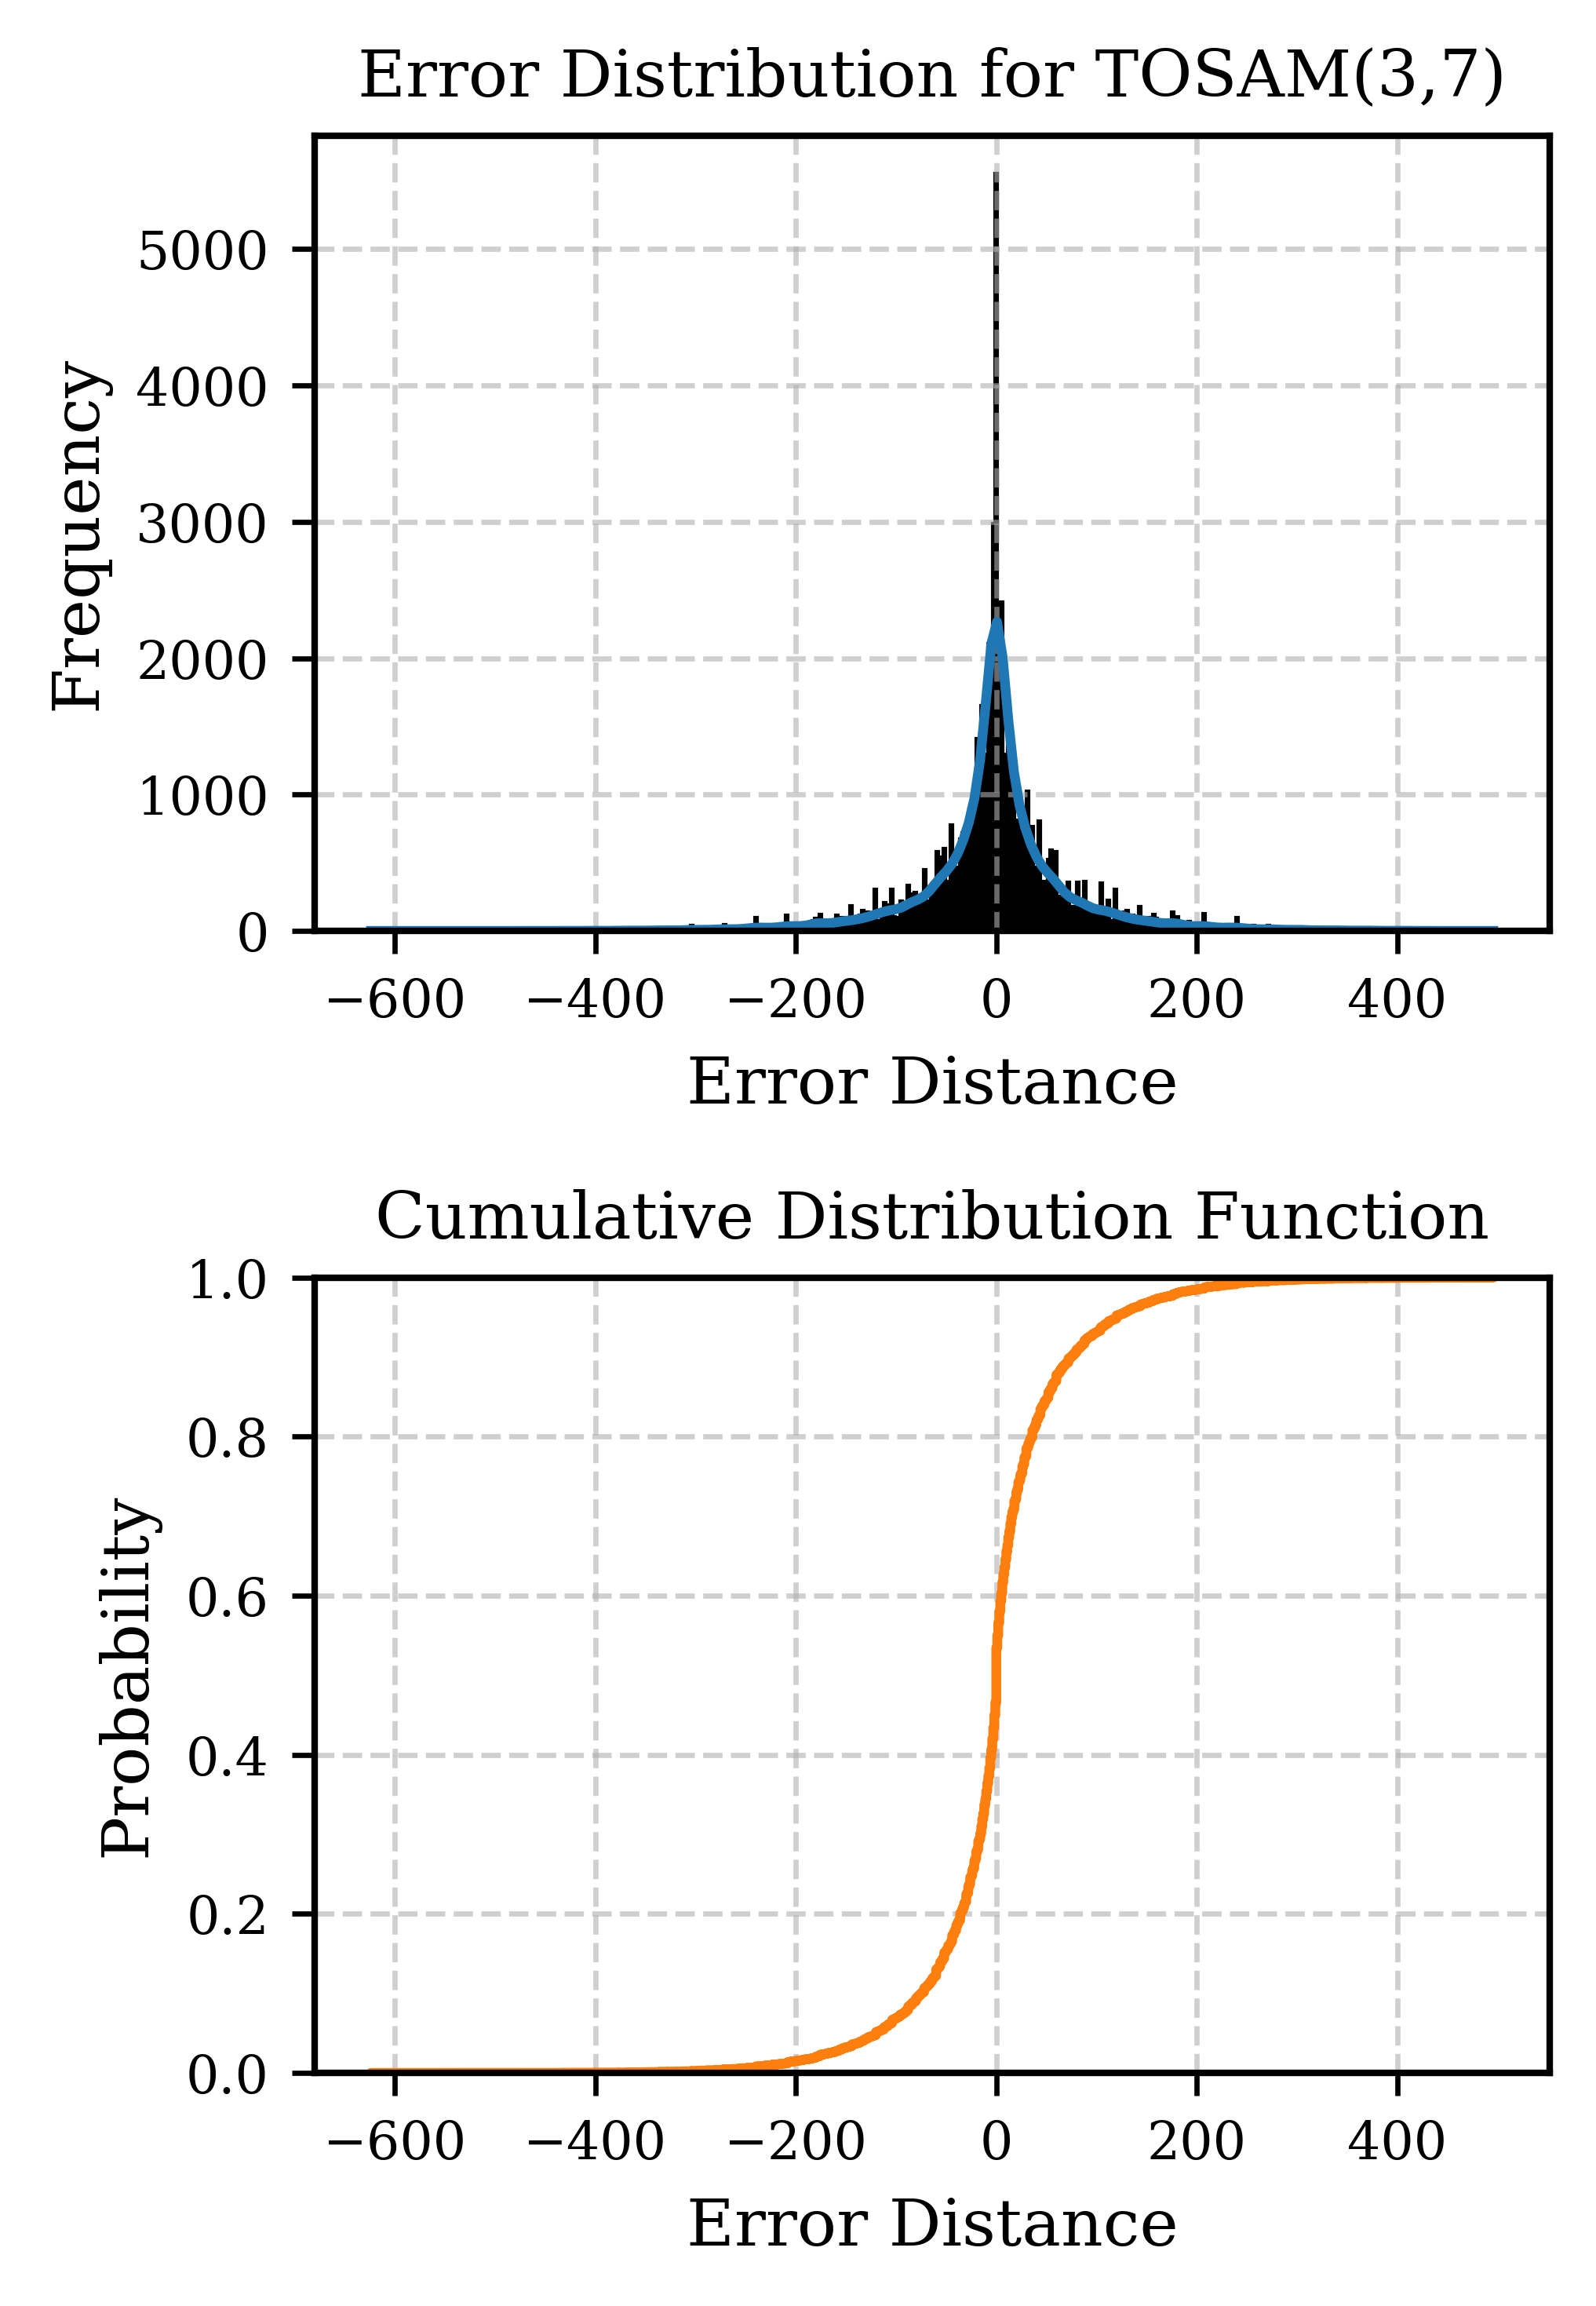
\includegraphics[width=\textwidth]{figures/08_tosam37_histogram.png}
        \caption{TOSAM$(3,7)$}
    \end{subfigure}
    \caption{四组 TOSAM 配置的误差直方图与经验累积分布对比}
    \label{fig:tosam-hist-grid}
\end{figure}

\begin{figure}[htbp]
    \centering
    \begin{subfigure}[b]{0.49\textwidth}
        \centering
        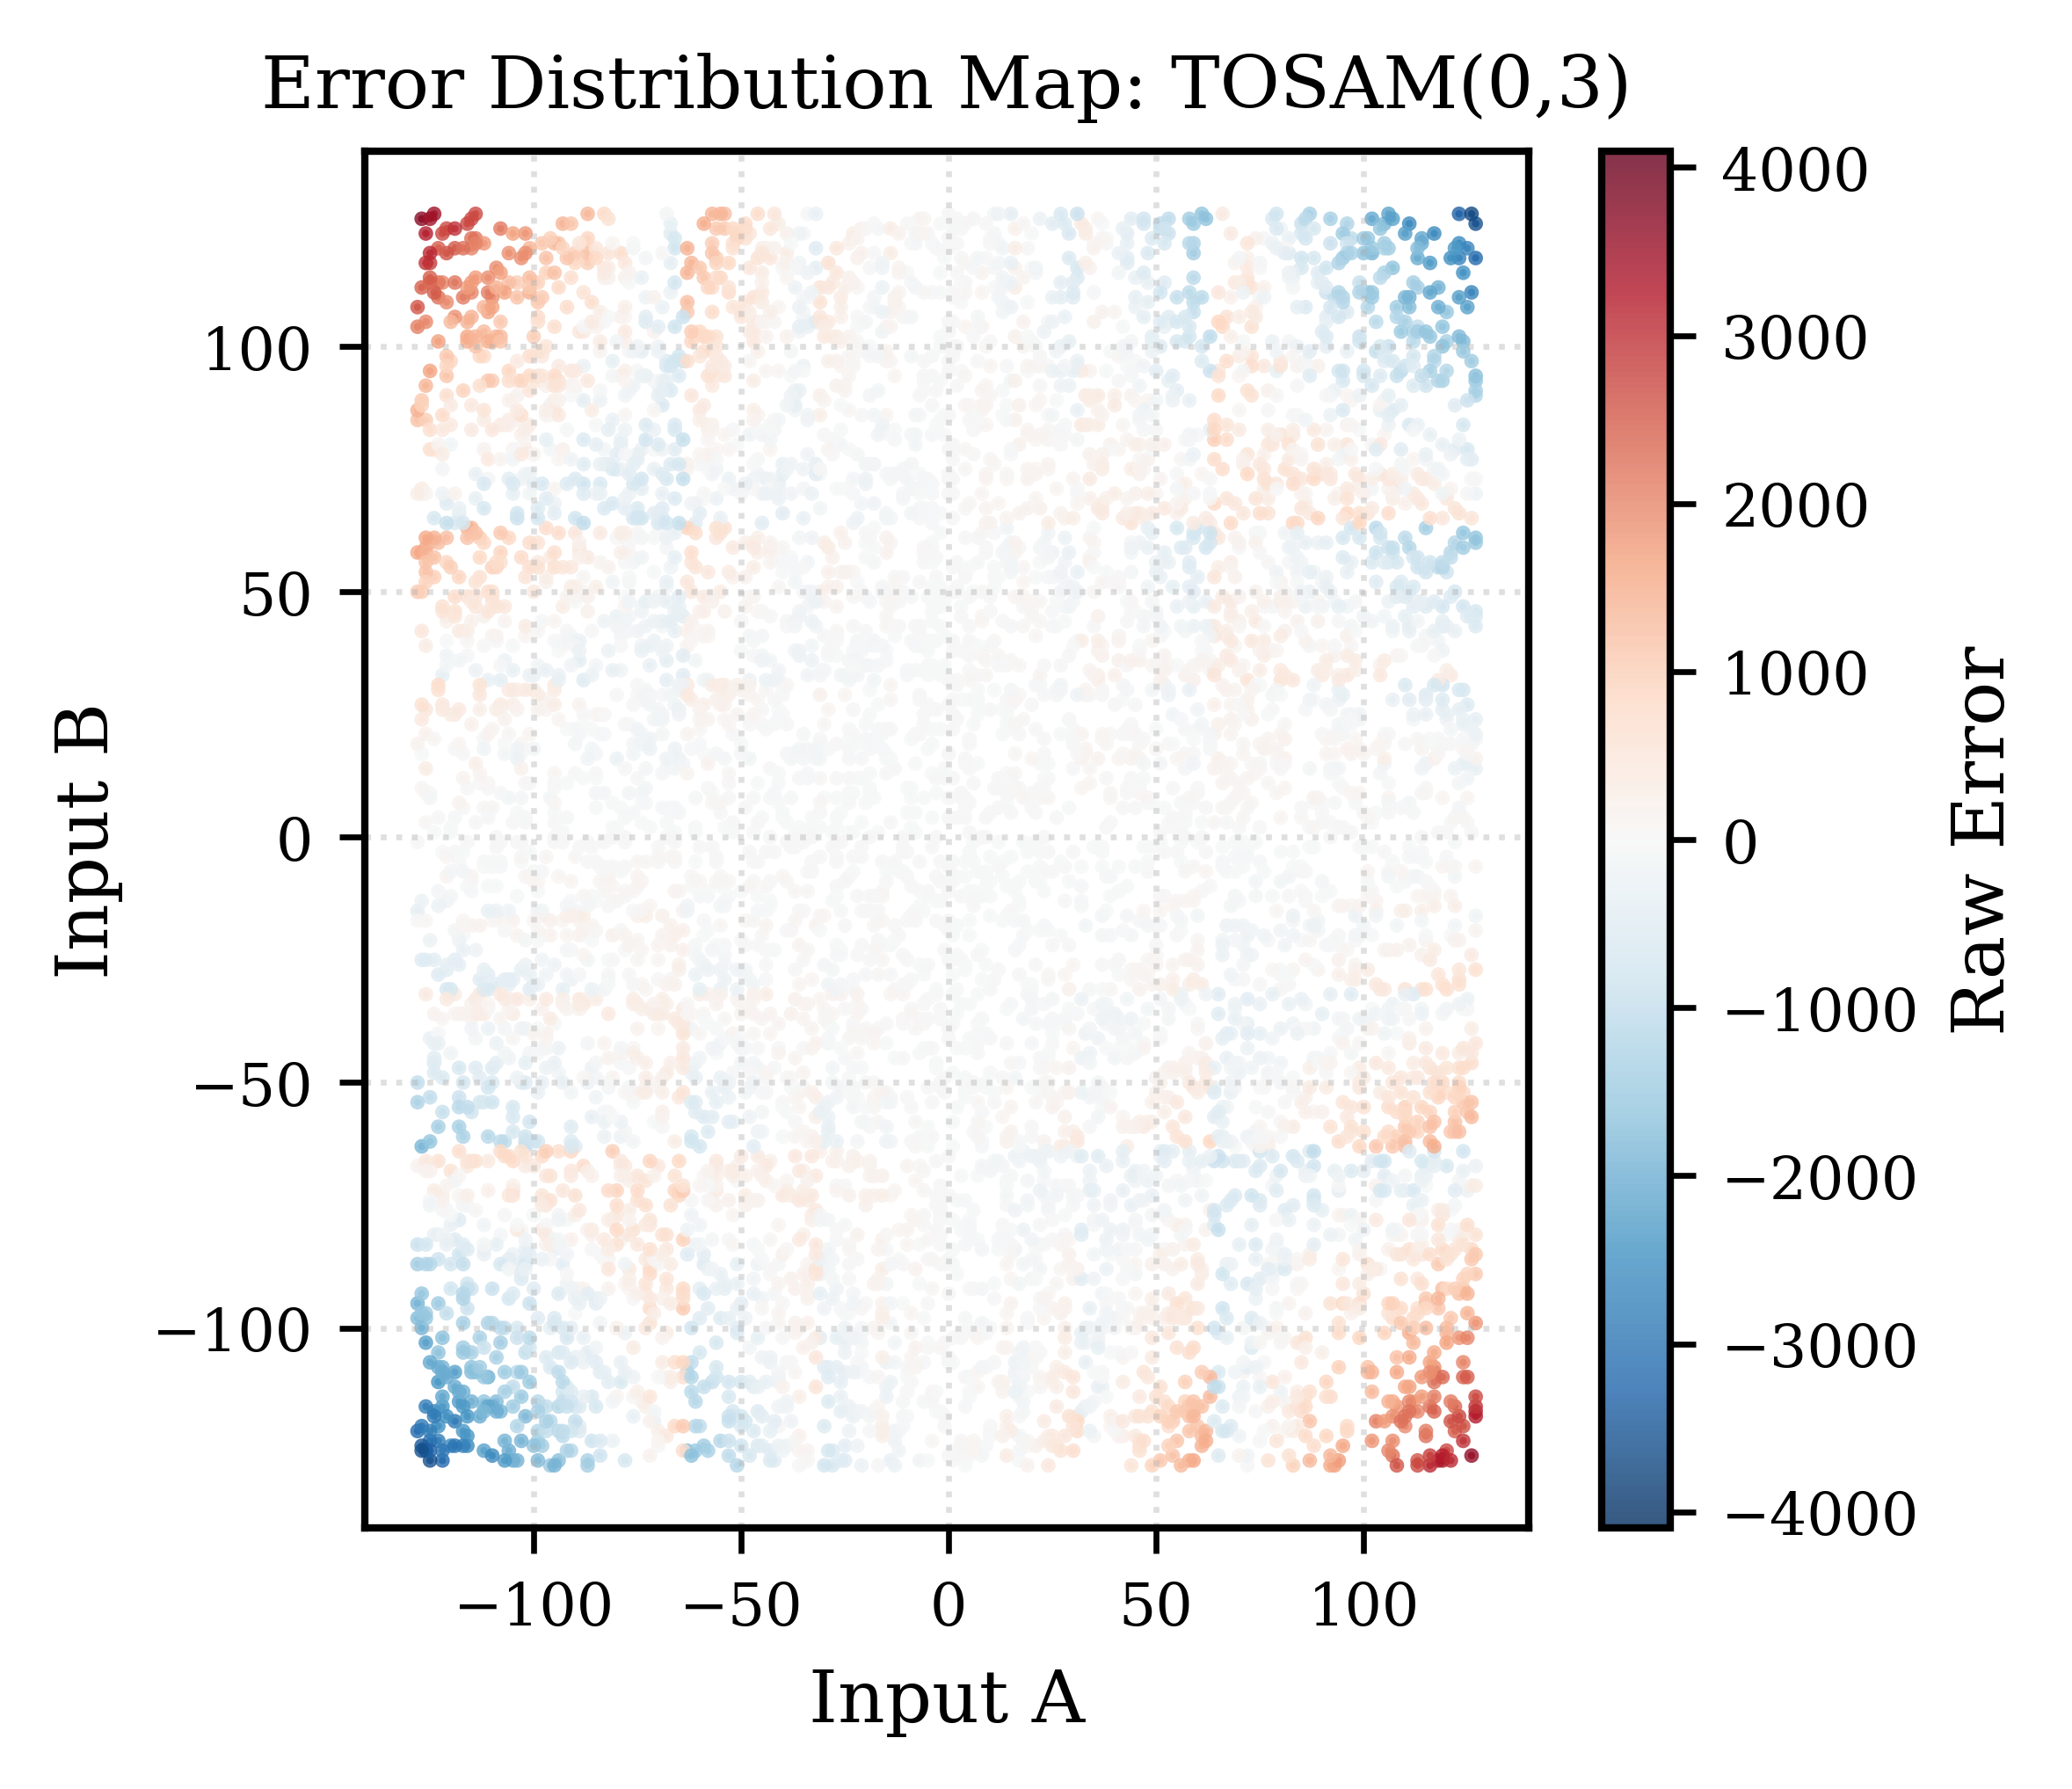
\includegraphics[width=\textwidth]{figures/08_tosam03_heatmap.png}
        \caption{TOSAM$(0,3)$}
    \end{subfigure}\hfill
    \begin{subfigure}[b]{0.49\textwidth}
        \centering
        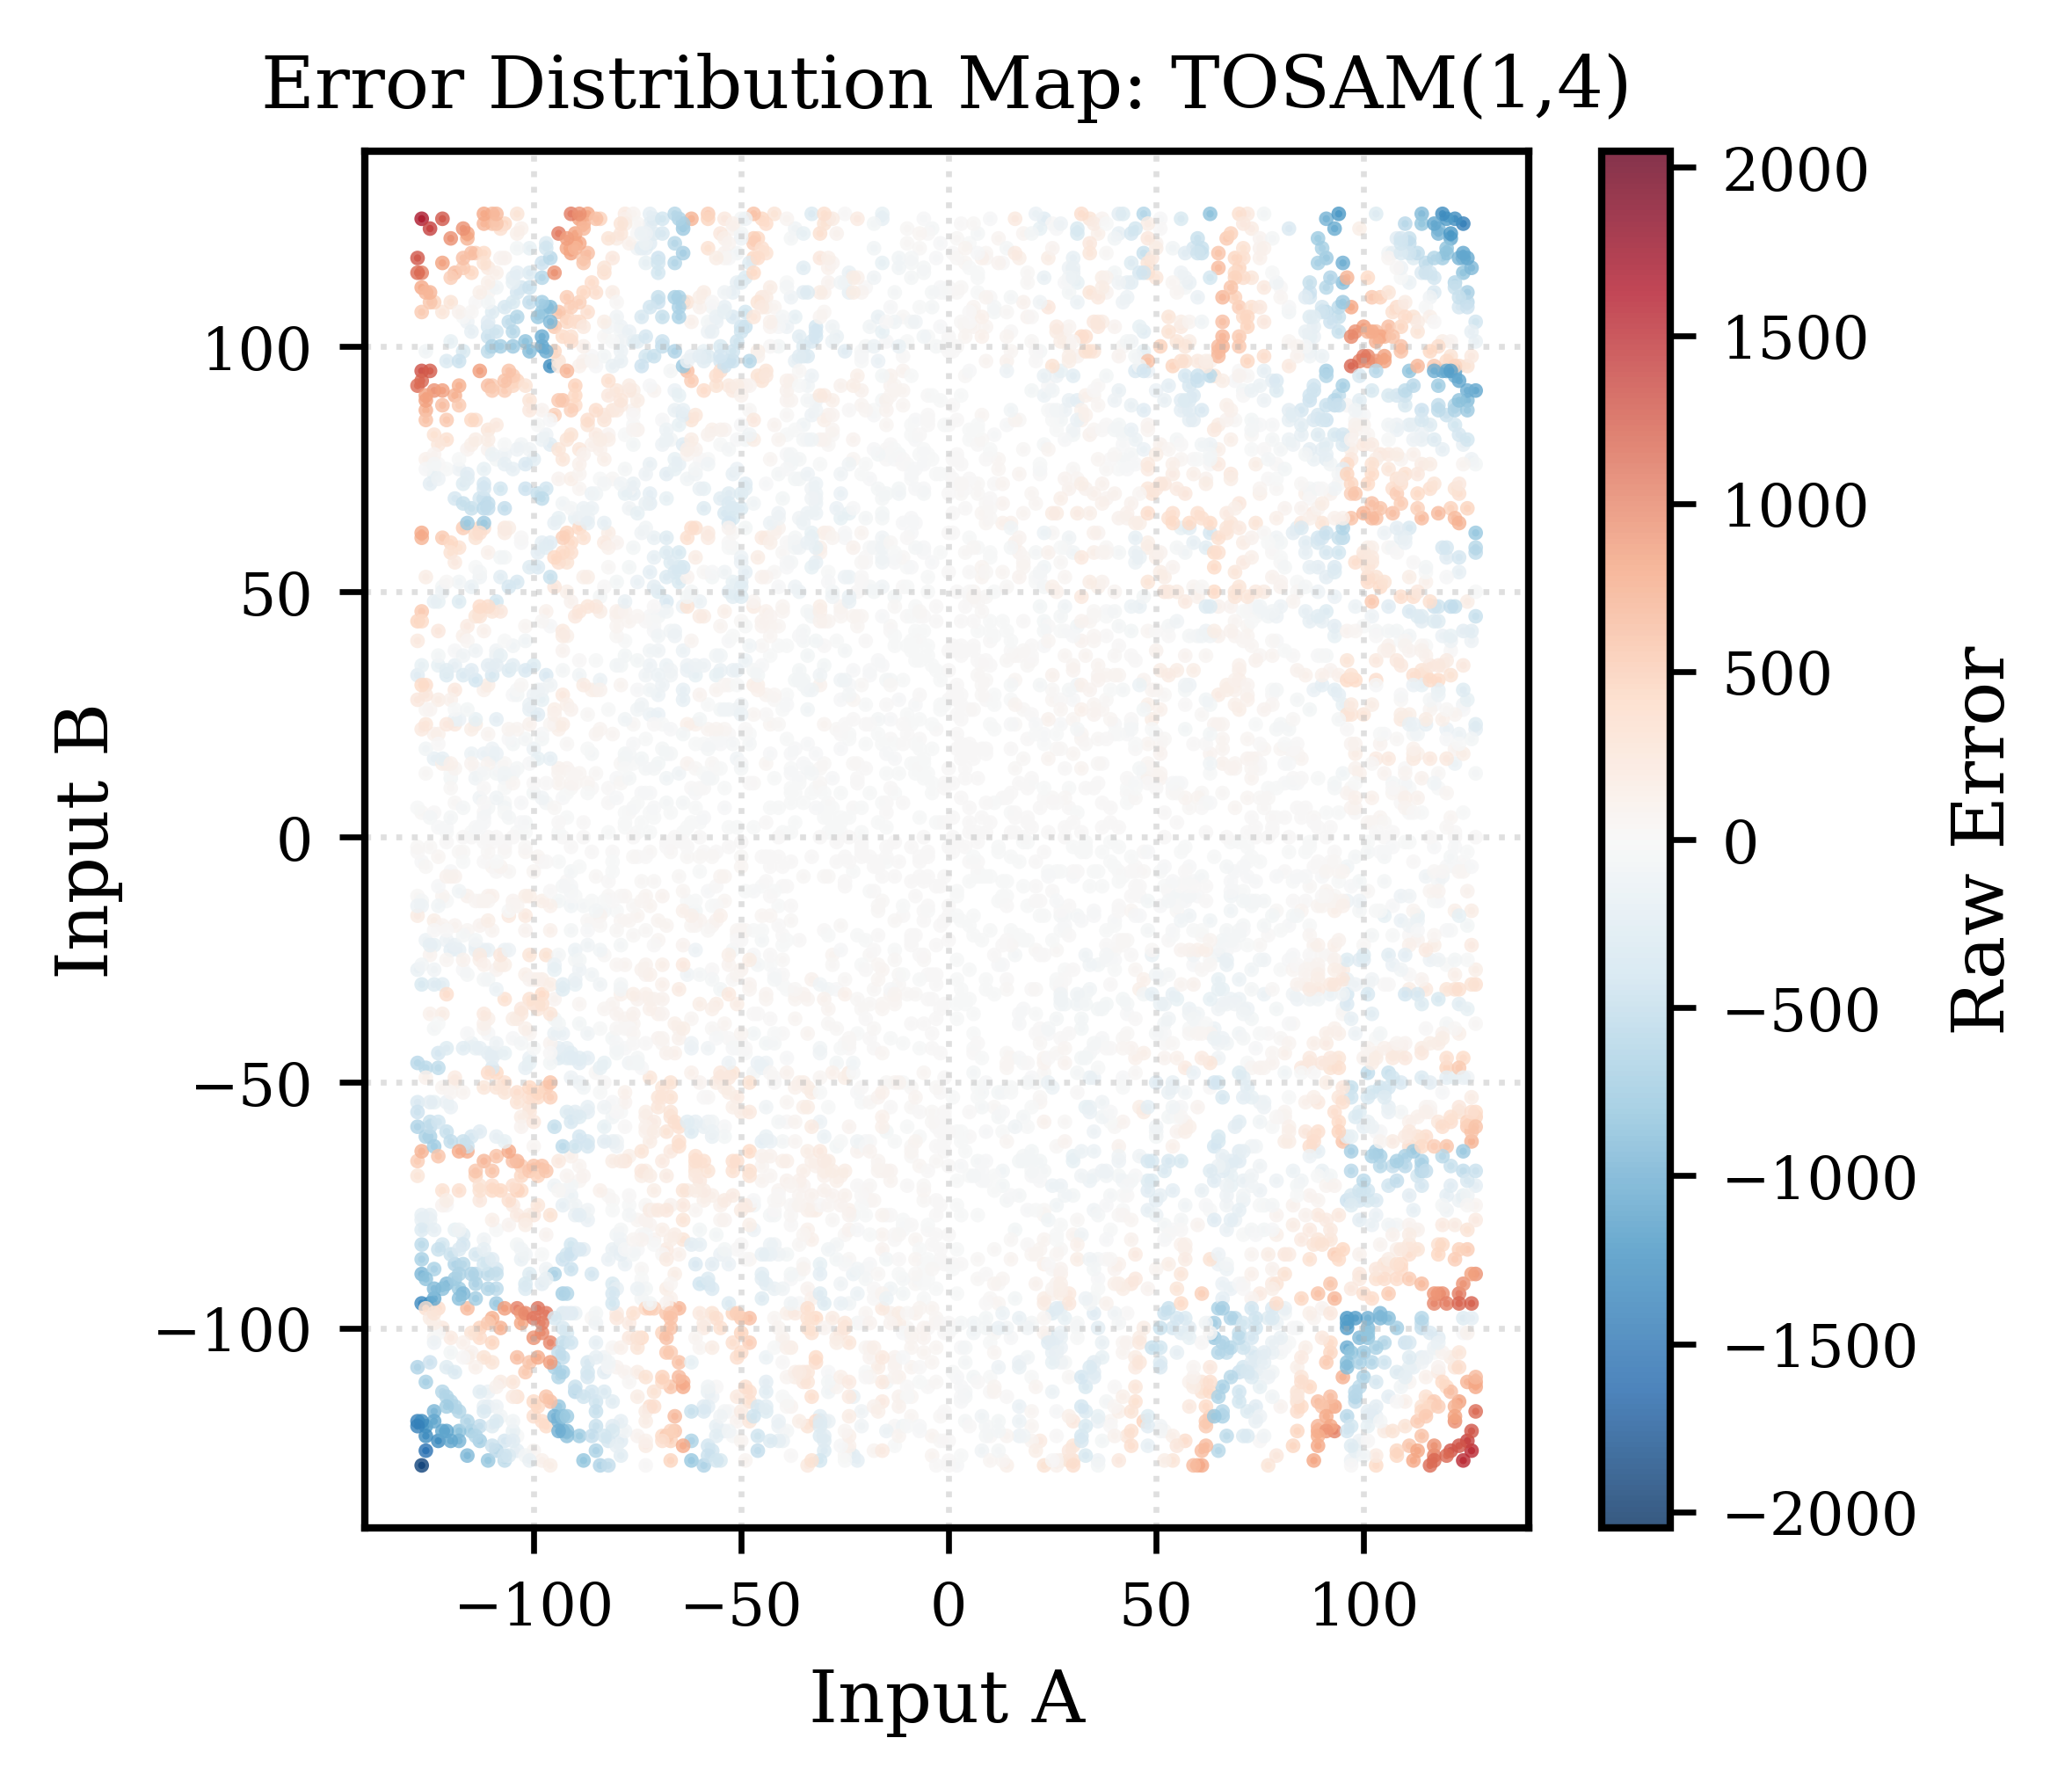
\includegraphics[width=\textwidth]{figures/08_tosam14_heatmap.png}
        \caption{TOSAM$(1,4)$}
    \end{subfigure}

    \vspace{0.2em}

    \begin{subfigure}[b]{0.49\textwidth}
        \centering
        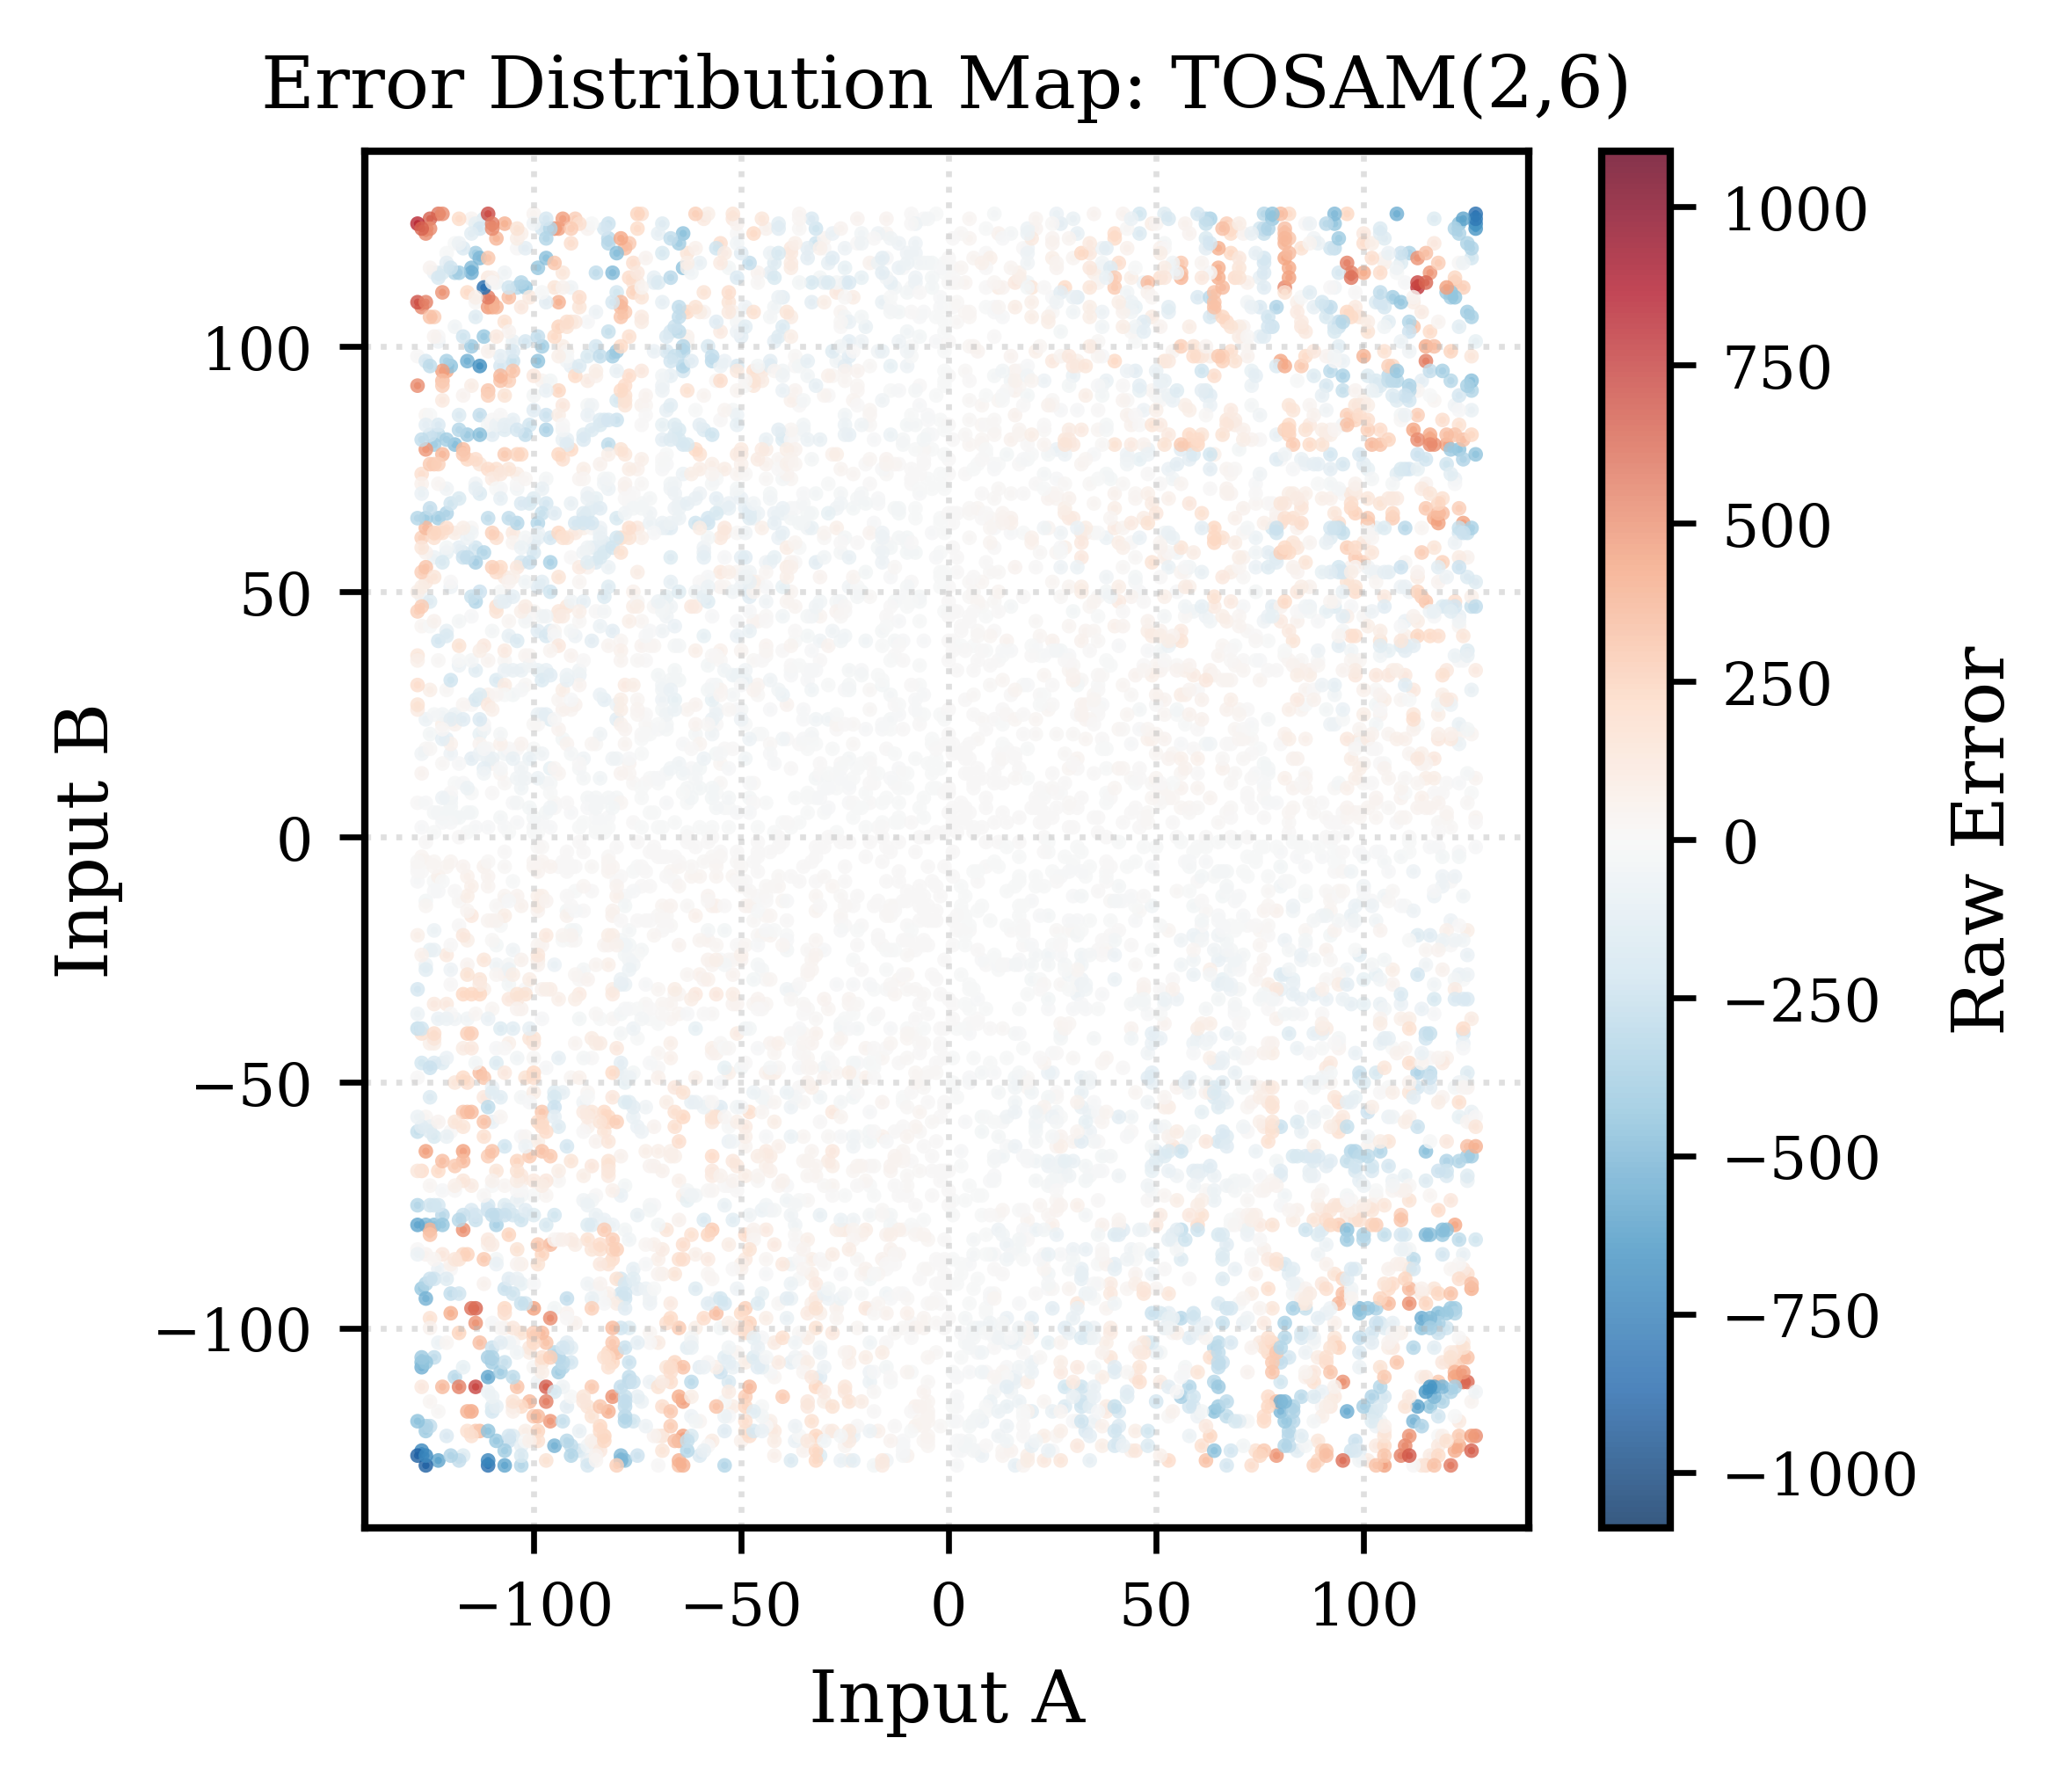
\includegraphics[width=\textwidth]{figures/08_tosam26_heatmap.png}
        \caption{TOSAM$(2,6)$}
    \end{subfigure}\hfill
    \begin{subfigure}[b]{0.49\textwidth}
        \centering
        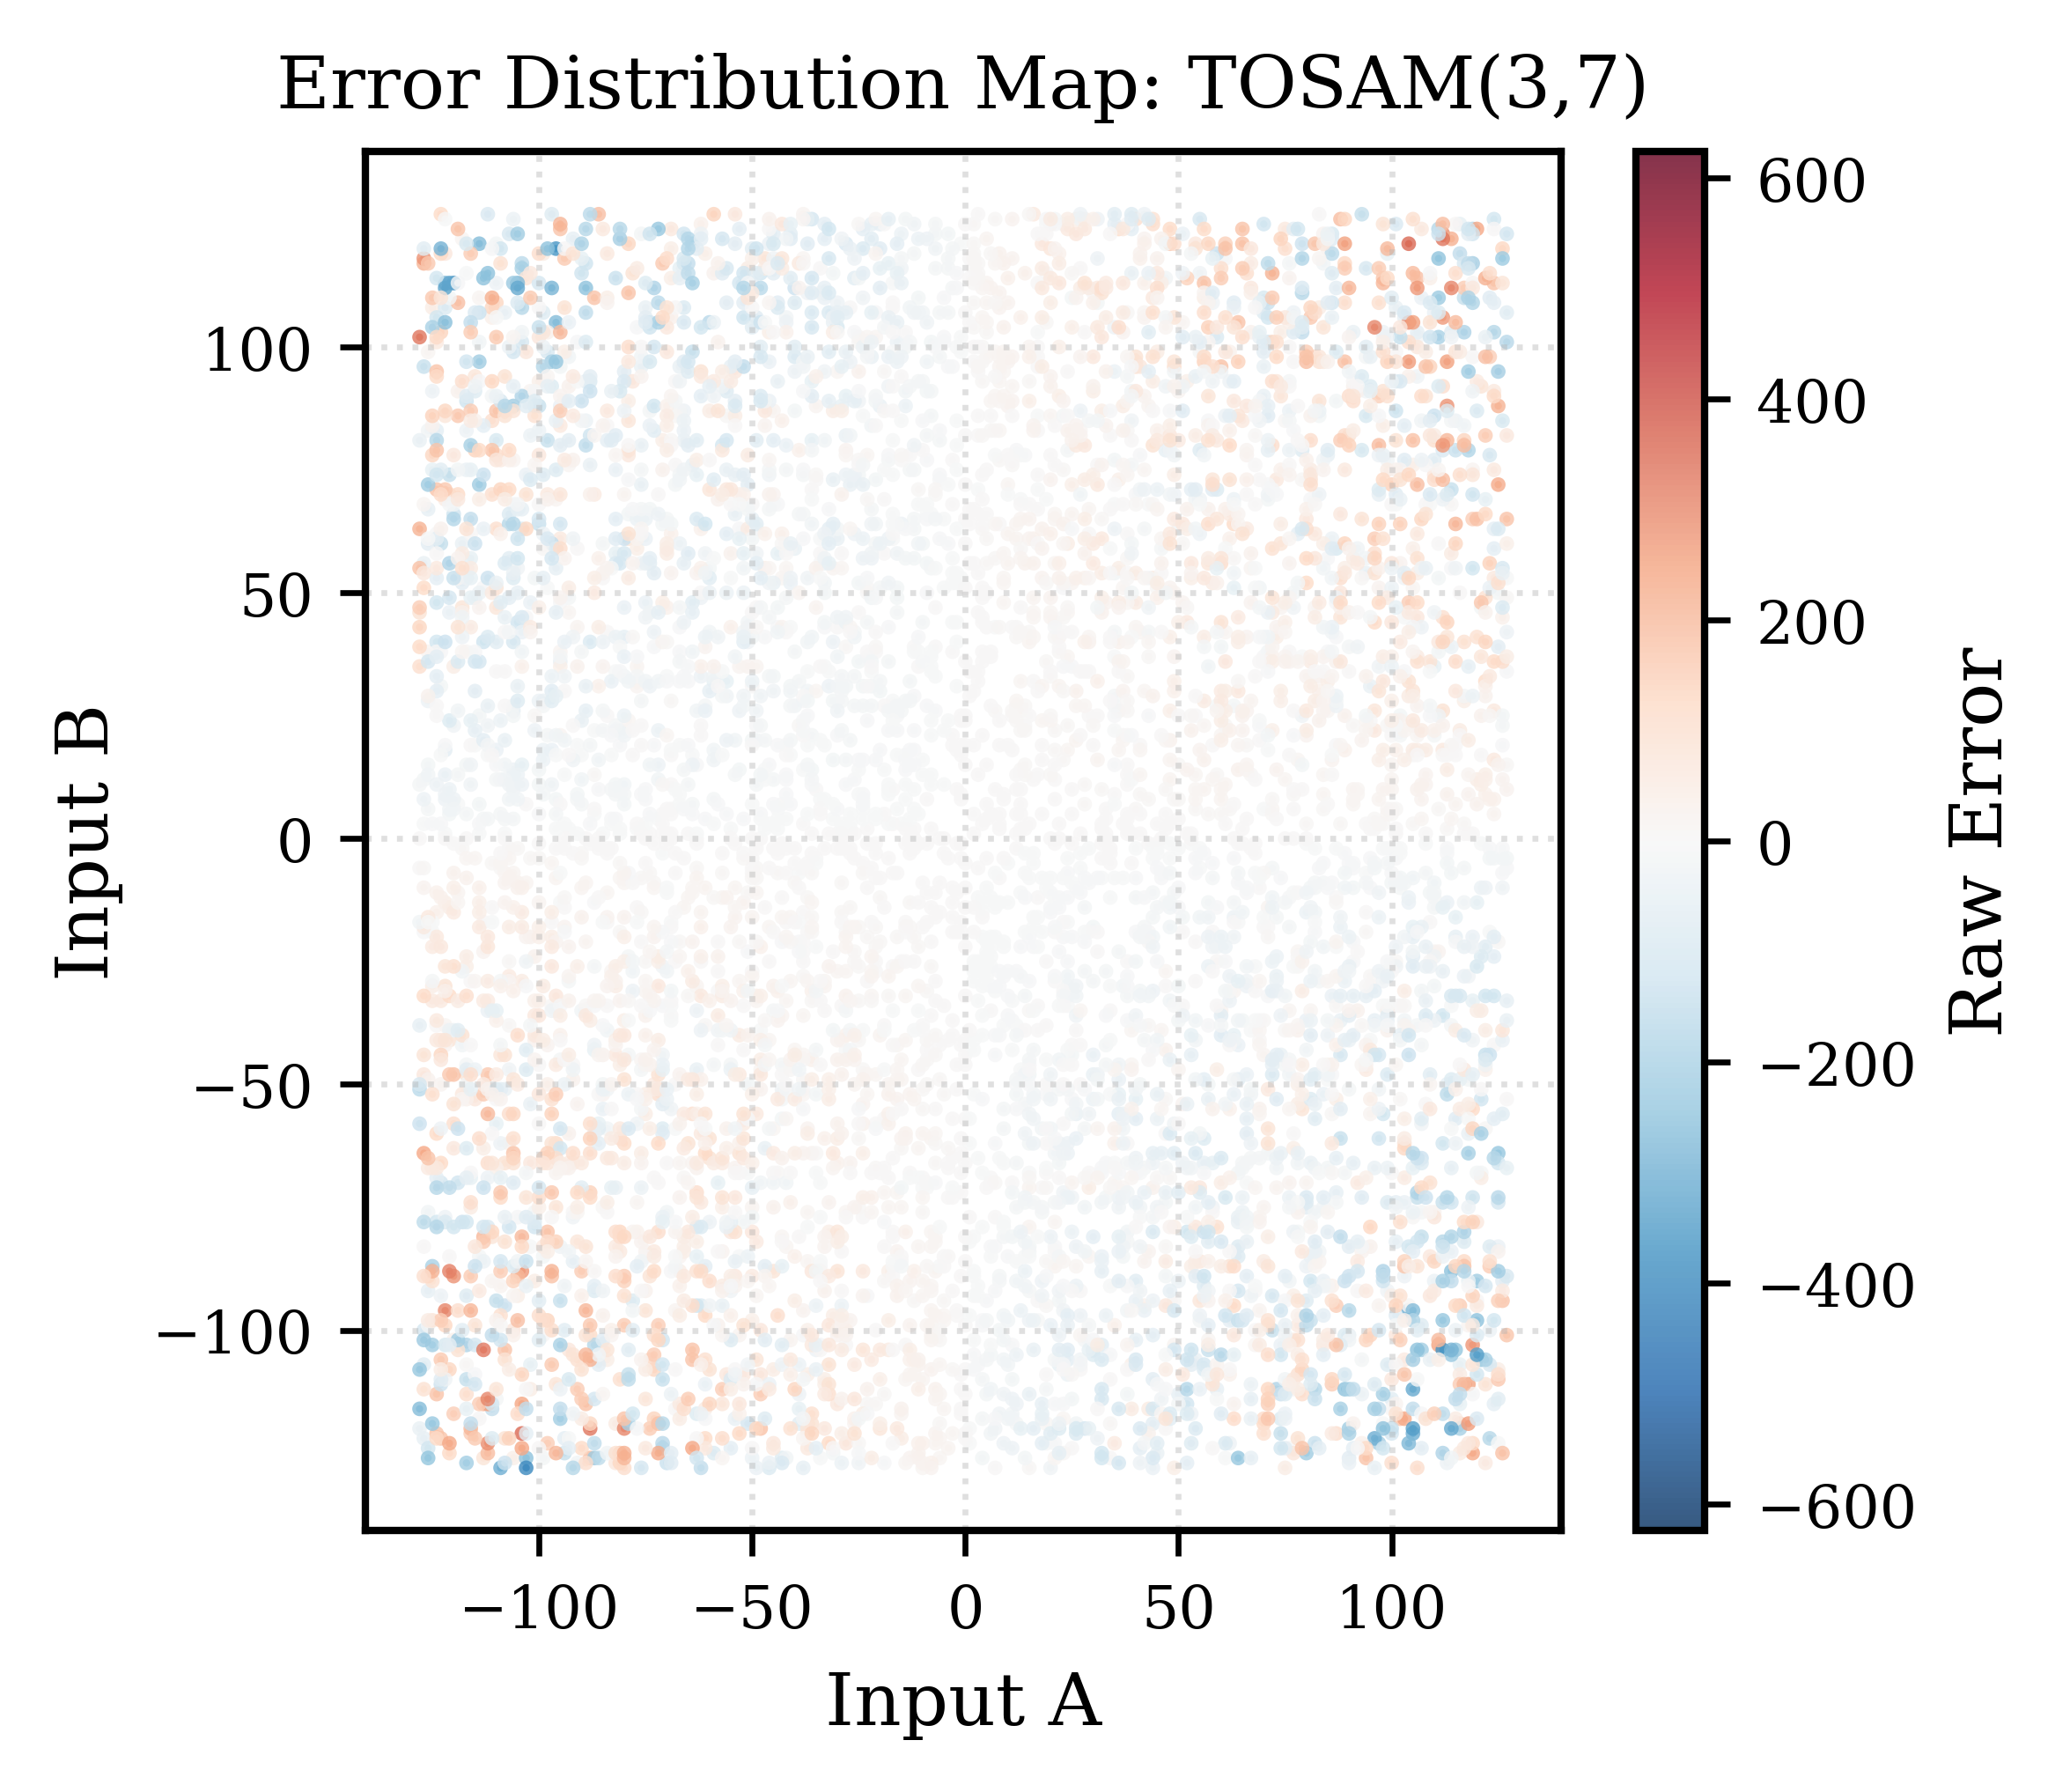
\includegraphics[width=\textwidth]{figures/08_tosam37_heatmap.png}
        \caption{TOSAM$(3,7)$}
    \end{subfigure}
    \caption{四组 TOSAM 配置在输入空间上的误差分布热力图对比}
    \label{fig:tosam-heat-grid}
\end{figure}

\clearpage
\subsubsection{ZBA-BM误差分析}
\label{subsec:zbabm-err}

针对 ZBA-BM 的算子级误差特性，本文对四组配置 \texttt{KMap\_4Row\_ZG}、ZBA-BM~0E4A、ZBA-BM~1E3A 与 ZBA-BM~2E2A 分别进行了 8 位有符号乘法全遍历分析。其中 \texttt{KMap\_4Row\_ZG} 与 0E4A 在近似深度上完全对齐——二者均对四行部分积全部启用 K-Map 化简，唯一差异在于是否启用 §\ref{subsec:zbabm-arch} 给出的 Row-0 选择性部分积补偿（PPSC）：前者剥除 PPSC，作为定位均值修正贡献的零补偿基线；后者保留 PPSC，与 1E3A、2E2A 一同覆盖典型的精度--PPA 调节范围。3E1A 与 4E0A 在精度上等价于精确 Booth，但因 K-Map 旁路 MUX 的引入反而恶化 PPA，无近似收益，故不纳入算子级对照。输入覆盖区间为 $[-128,127]$，共得到 $65\,536$ 组样本；对每组样本同时计算精确乘积与近似乘积，并以
\(
e_{\mathrm{raw}}=P_{\mathrm{apx}}-P_{\mathrm{exact}}
\)
为基础统计 MAE、RMSE、相对误差、最坏误差及误差分位点，同时结合误差直方图与输入空间热力图观察误差在全输入域内的分布特征。

\begin{table}[htbp]
    \centering
    \caption{四组 ZBA-BM 配置的全遍历误差统计对比}
    \label{tab:zbabm-variants-err}
    \small
    \setlength{\tabcolsep}{5pt}
    \begin{tabular}{lcccc}
        \toprule
        指标 & \texttt{KMap\_4Row\_ZG} & ZBA-BM 0E4A & ZBA-BM 1E3A & ZBA-BM 2E2A \\
        \midrule
        ME      & $-0.1250$ & $+0.0000$ & $+0.0000$ & $+0.0000$ \\
        MAE     & $1180.50$ & $1176.00$ & $288.00$  & $64.00$ \\
        RMSE    & $2284.69$ & $2284.99$ & $572.44$  & $147.80$ \\
        MARE    & $23.53\%$ & $22.96\%$ & $10.63\%$ & $3.21\%$ \\
        WRE     & $59.81\%$ & $66.67\%$ & $66.67\%$ & $66.67\%$ \\
        WAE     & $8704$    & $8704$    & $2048$    & $512$ \\
        $P99_{\mathrm{raw}}$ & $7698$ & $7723$ & $1936$ & $492$ \\
        Sign Errors & $0$ & $0$ & $0$ & $0$ \\
        \bottomrule
    \end{tabular}
\end{table}

表~\ref{tab:zbabm-variants-err} 给出了四组配置的统一统计结果。可以看出，在 4 行全近似深度下，
\texttt{KMap\_4Row\_ZG} 的中位误差为 $-0.125$，精确复现前述 Row-0 偏差溯源中的解析值 $\mu_
{\text{row-0}}=-1/8$，而 ZBA-BM 0E4A 在同等近似深度下将该指标压回严格的 $0$；两者的 MAE
（$1180.50$ 与 $1176.00$）、RMSE（$2284.69$ 与 $2284.99$）等方差侧指标差距均不超过 $0.4\%$，
说明 PPSC 仅以一个 Row-0 旁路 MUX 即修正了 $\mu_{\text{row-0}}$，而几乎不在方差侧引入额外代价。
随着近似行数由 4 行收缩到 3 行、2 行，ZBA-BM 1E3A 与 2E2A 的 MAE 进一步下降至 $288.00$ 与 $64.00$，
RMSE 由 $2284.99$ 收缩至 $147.80$，$P99_{\mathrm{raw}}$ 由 $7723$ 收缩至 $492$，误差包
络近两个数量级地内缩；期间 ME 始终保持为 $0$，说明零均值性质与近似行数解耦，不随精度设置退化。
与此同时，所有四组配置的 Zero Errors 与 Sign Errors 均为 $0$，说明 K-Map 化简在去除冗余项后仍保
持 8 位有符号乘积的零保持与符号一致性，此即前述零编码守恒项 $\neg\mathtt{zero}$ 约束在算子级的直接体现。对于矩阵乘法这类累加深度较高的场景，4 行近似配置的 MAE 与高分位误差仍然偏大，经过多次乘加累积后容易放大为不可忽略的输出偏差，故纯 0E4A 配置仅适用于浅层累加；1E3A 与 2E2A 通过保留首行/前两行精确，在算子级即将方差侧指标控制到适合较深累加链的水平。

从图~\ref{fig:zbabm-hist-grid}--图~\ref{fig:zbabm-heat-grid} 也可以直观看到这一变化规律。\texttt{KMap\_4Row\_ZG} 的直方图整体相对零位左偏一格，经验累积分布在零点处的偏移即对应 $\mu=-0.125$ 的固化偏差；ZBA-BM 0E4A 的直方图在不显著改变方差包络的前提下将中心拉回零位，呈现严格关于零对称的分布形态。随着近似行数减少，ZBA-BM 1E3A 与 2E2A 的直方图尾部依次收紧，热力图中高误差点在大幅值输入区域逐步退散，误差主体向中心收缩，$(a,b)$ 输入空间边缘的高误差区域亦得到有效压缩。基于这一结果，后续系统级与应用级验证将以 ZBA-BM 0E4A、1E3A、2E2A 三种精度设置作为候选配置参与多深度对比；\texttt{KMap\_4Row\_ZG} 不进入候选，仅作为定位 PPSC 均值修正贡献的零补偿基线保留在算子级对照中。

\begin{figure}[htbp]
    \centering
    \begin{subfigure}[b]{0.46\textwidth}
        \centering
        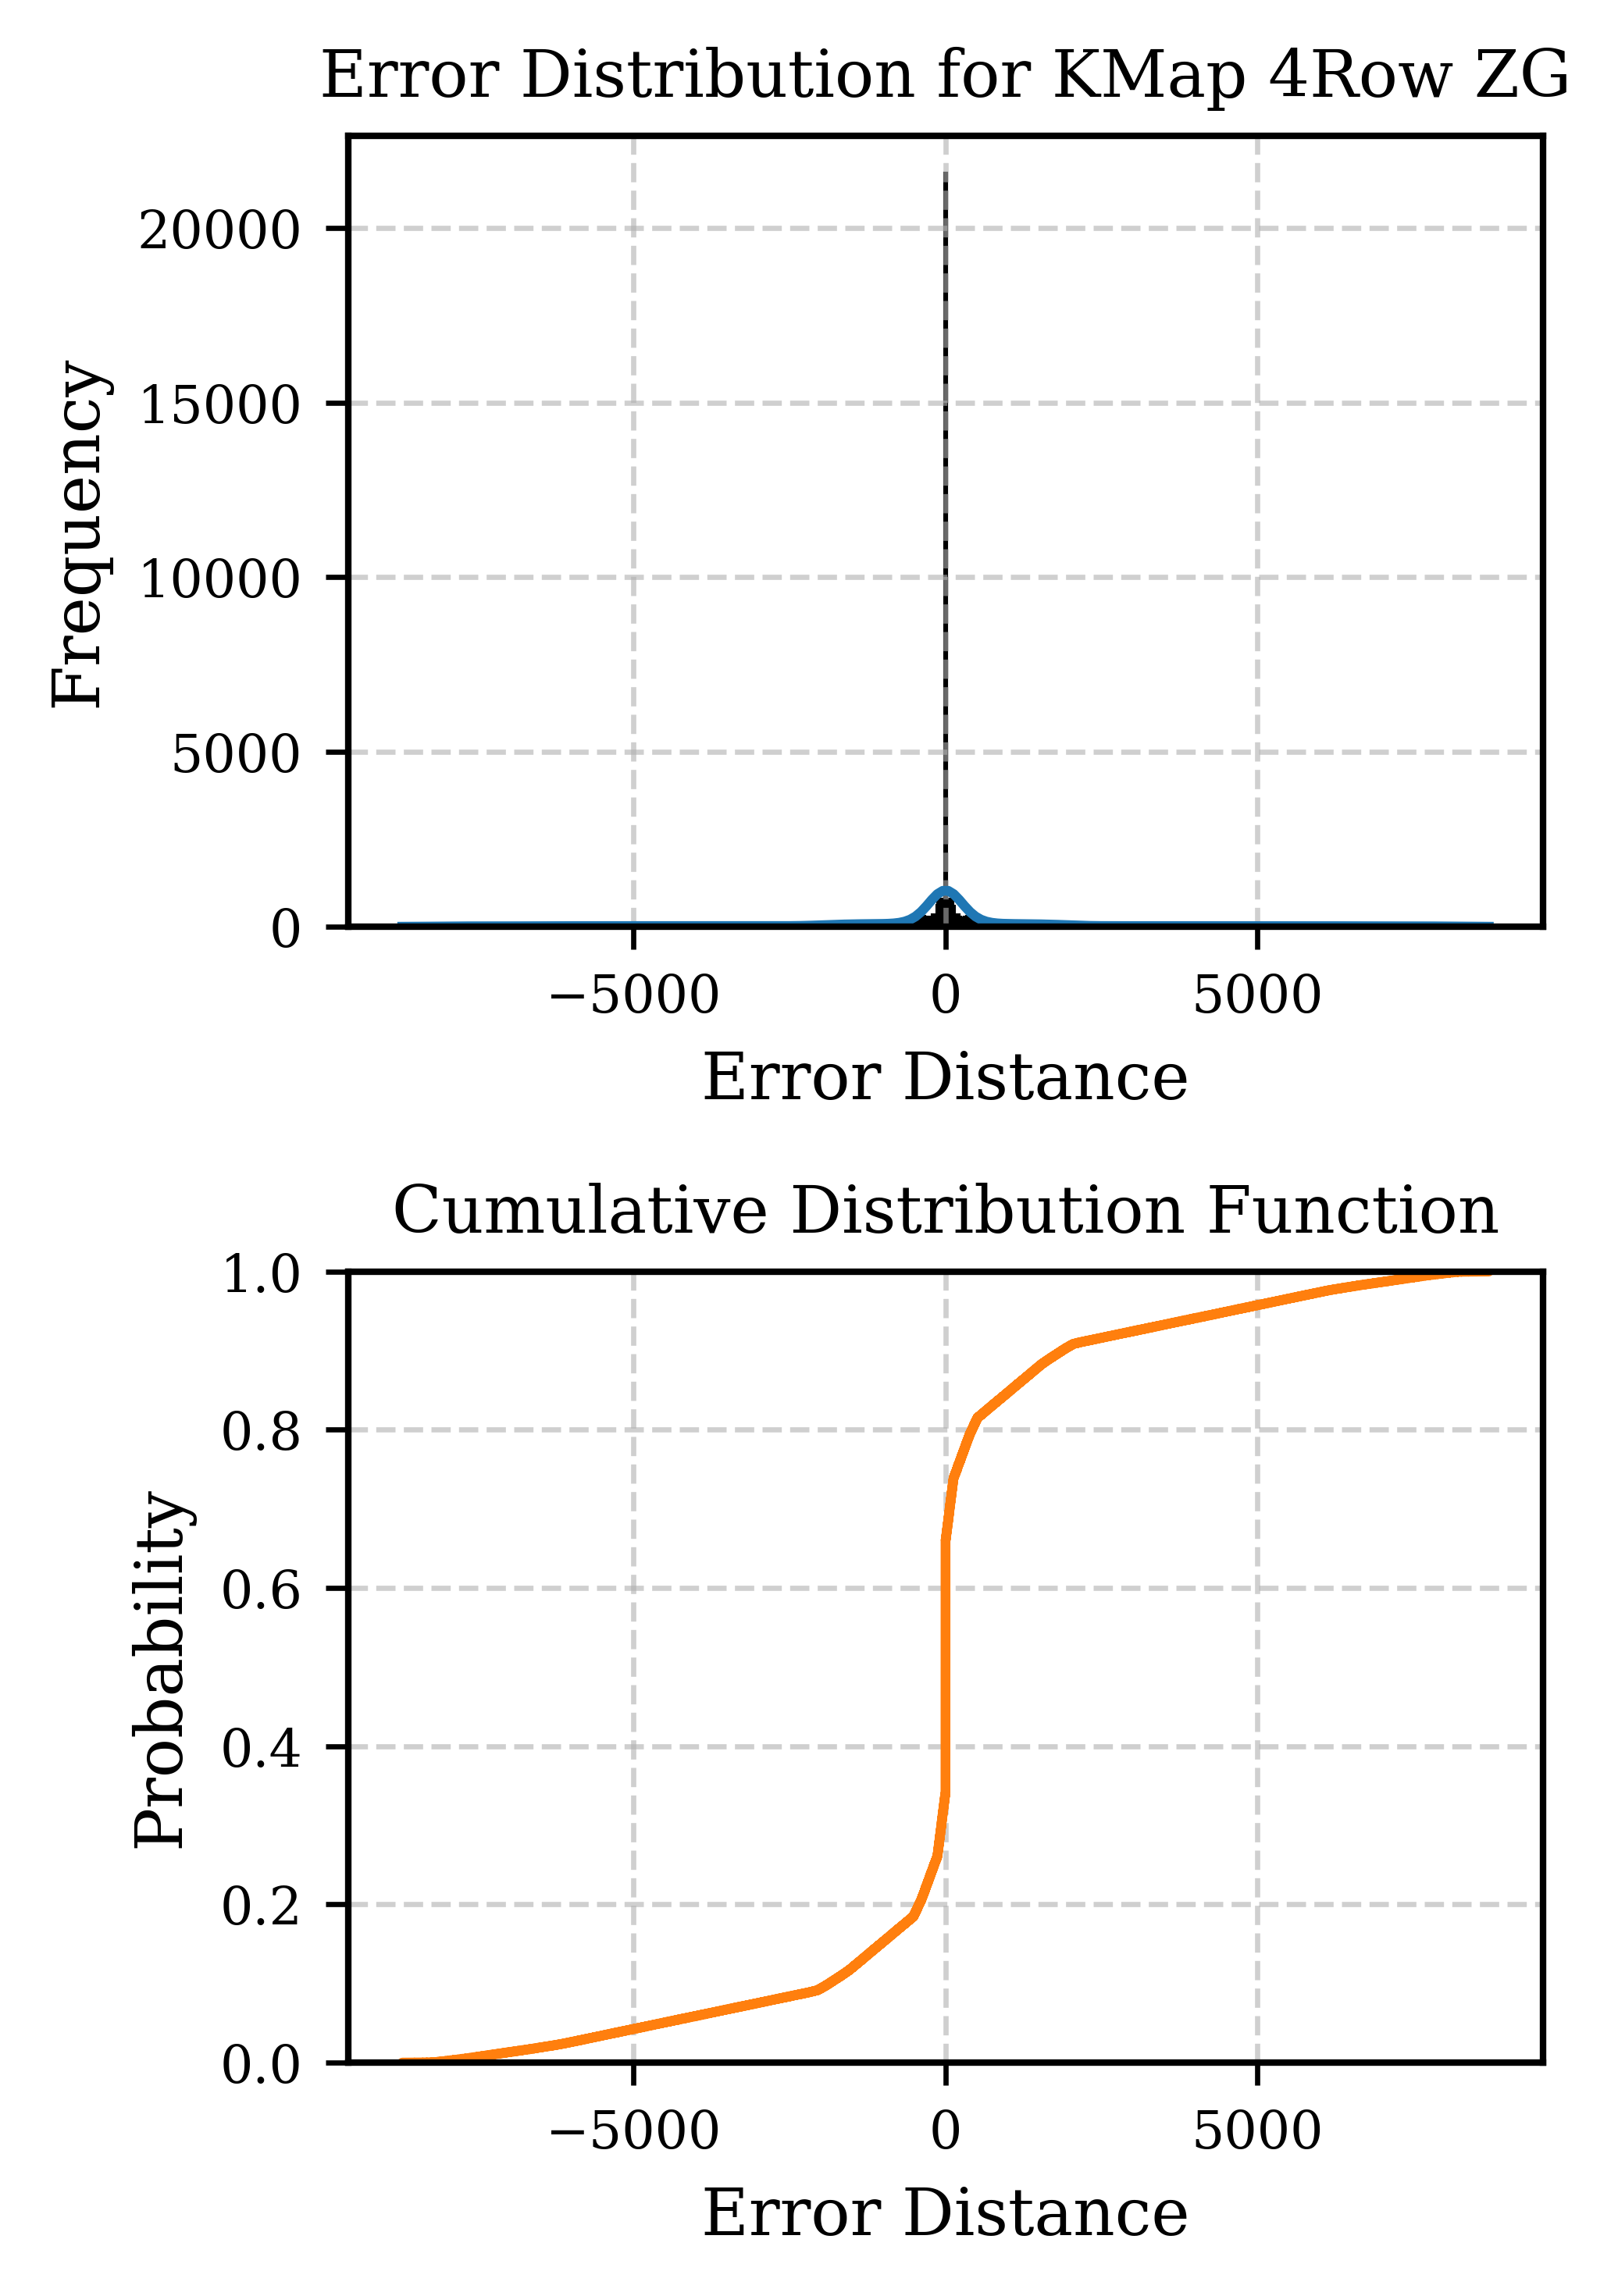
\includegraphics[width=\textwidth]{09_zbabm_4row_zg_histogram.png}
        \caption{\texttt{KMap\_4Row\_ZG}}
    \end{subfigure}\hfill
    \begin{subfigure}[b]{0.46\textwidth}
        \centering
        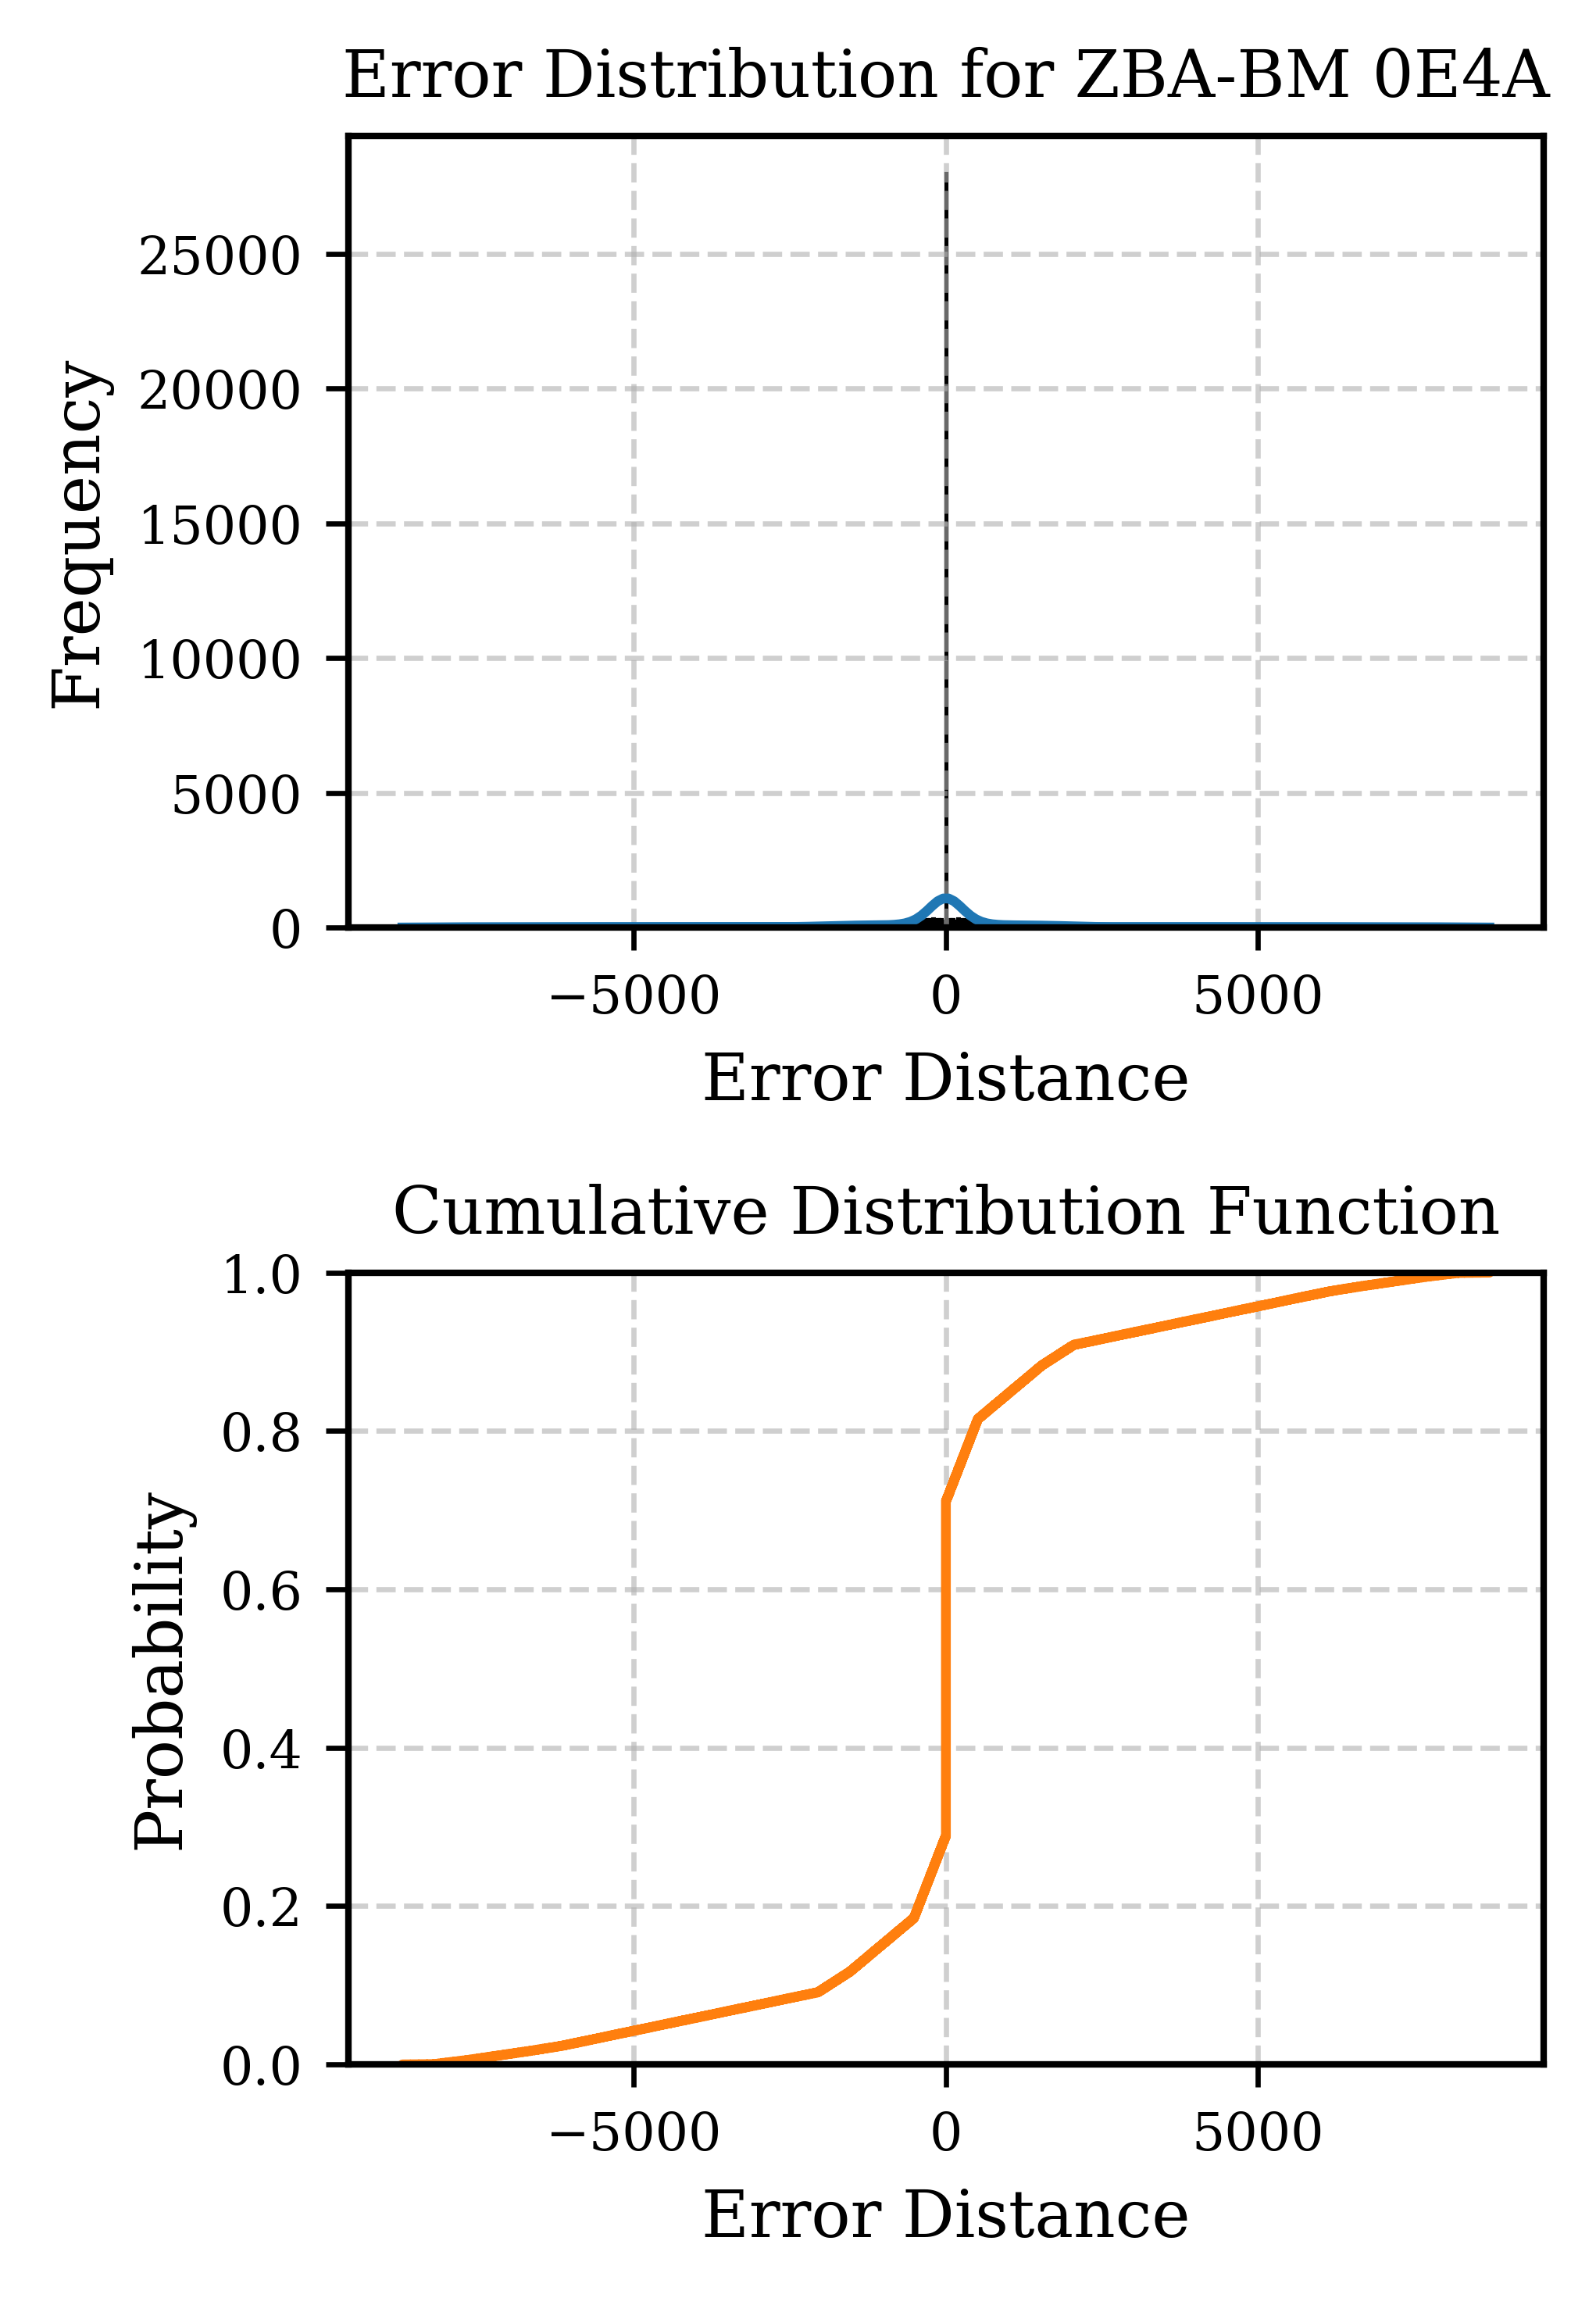
\includegraphics[width=\textwidth]{09_zbabm_0e4a_histogram.png}
        \caption{ZBA-BM 0E4A}
    \end{subfigure}

    \vspace{0.2em}

    \begin{subfigure}[b]{0.46\textwidth}
        \centering
        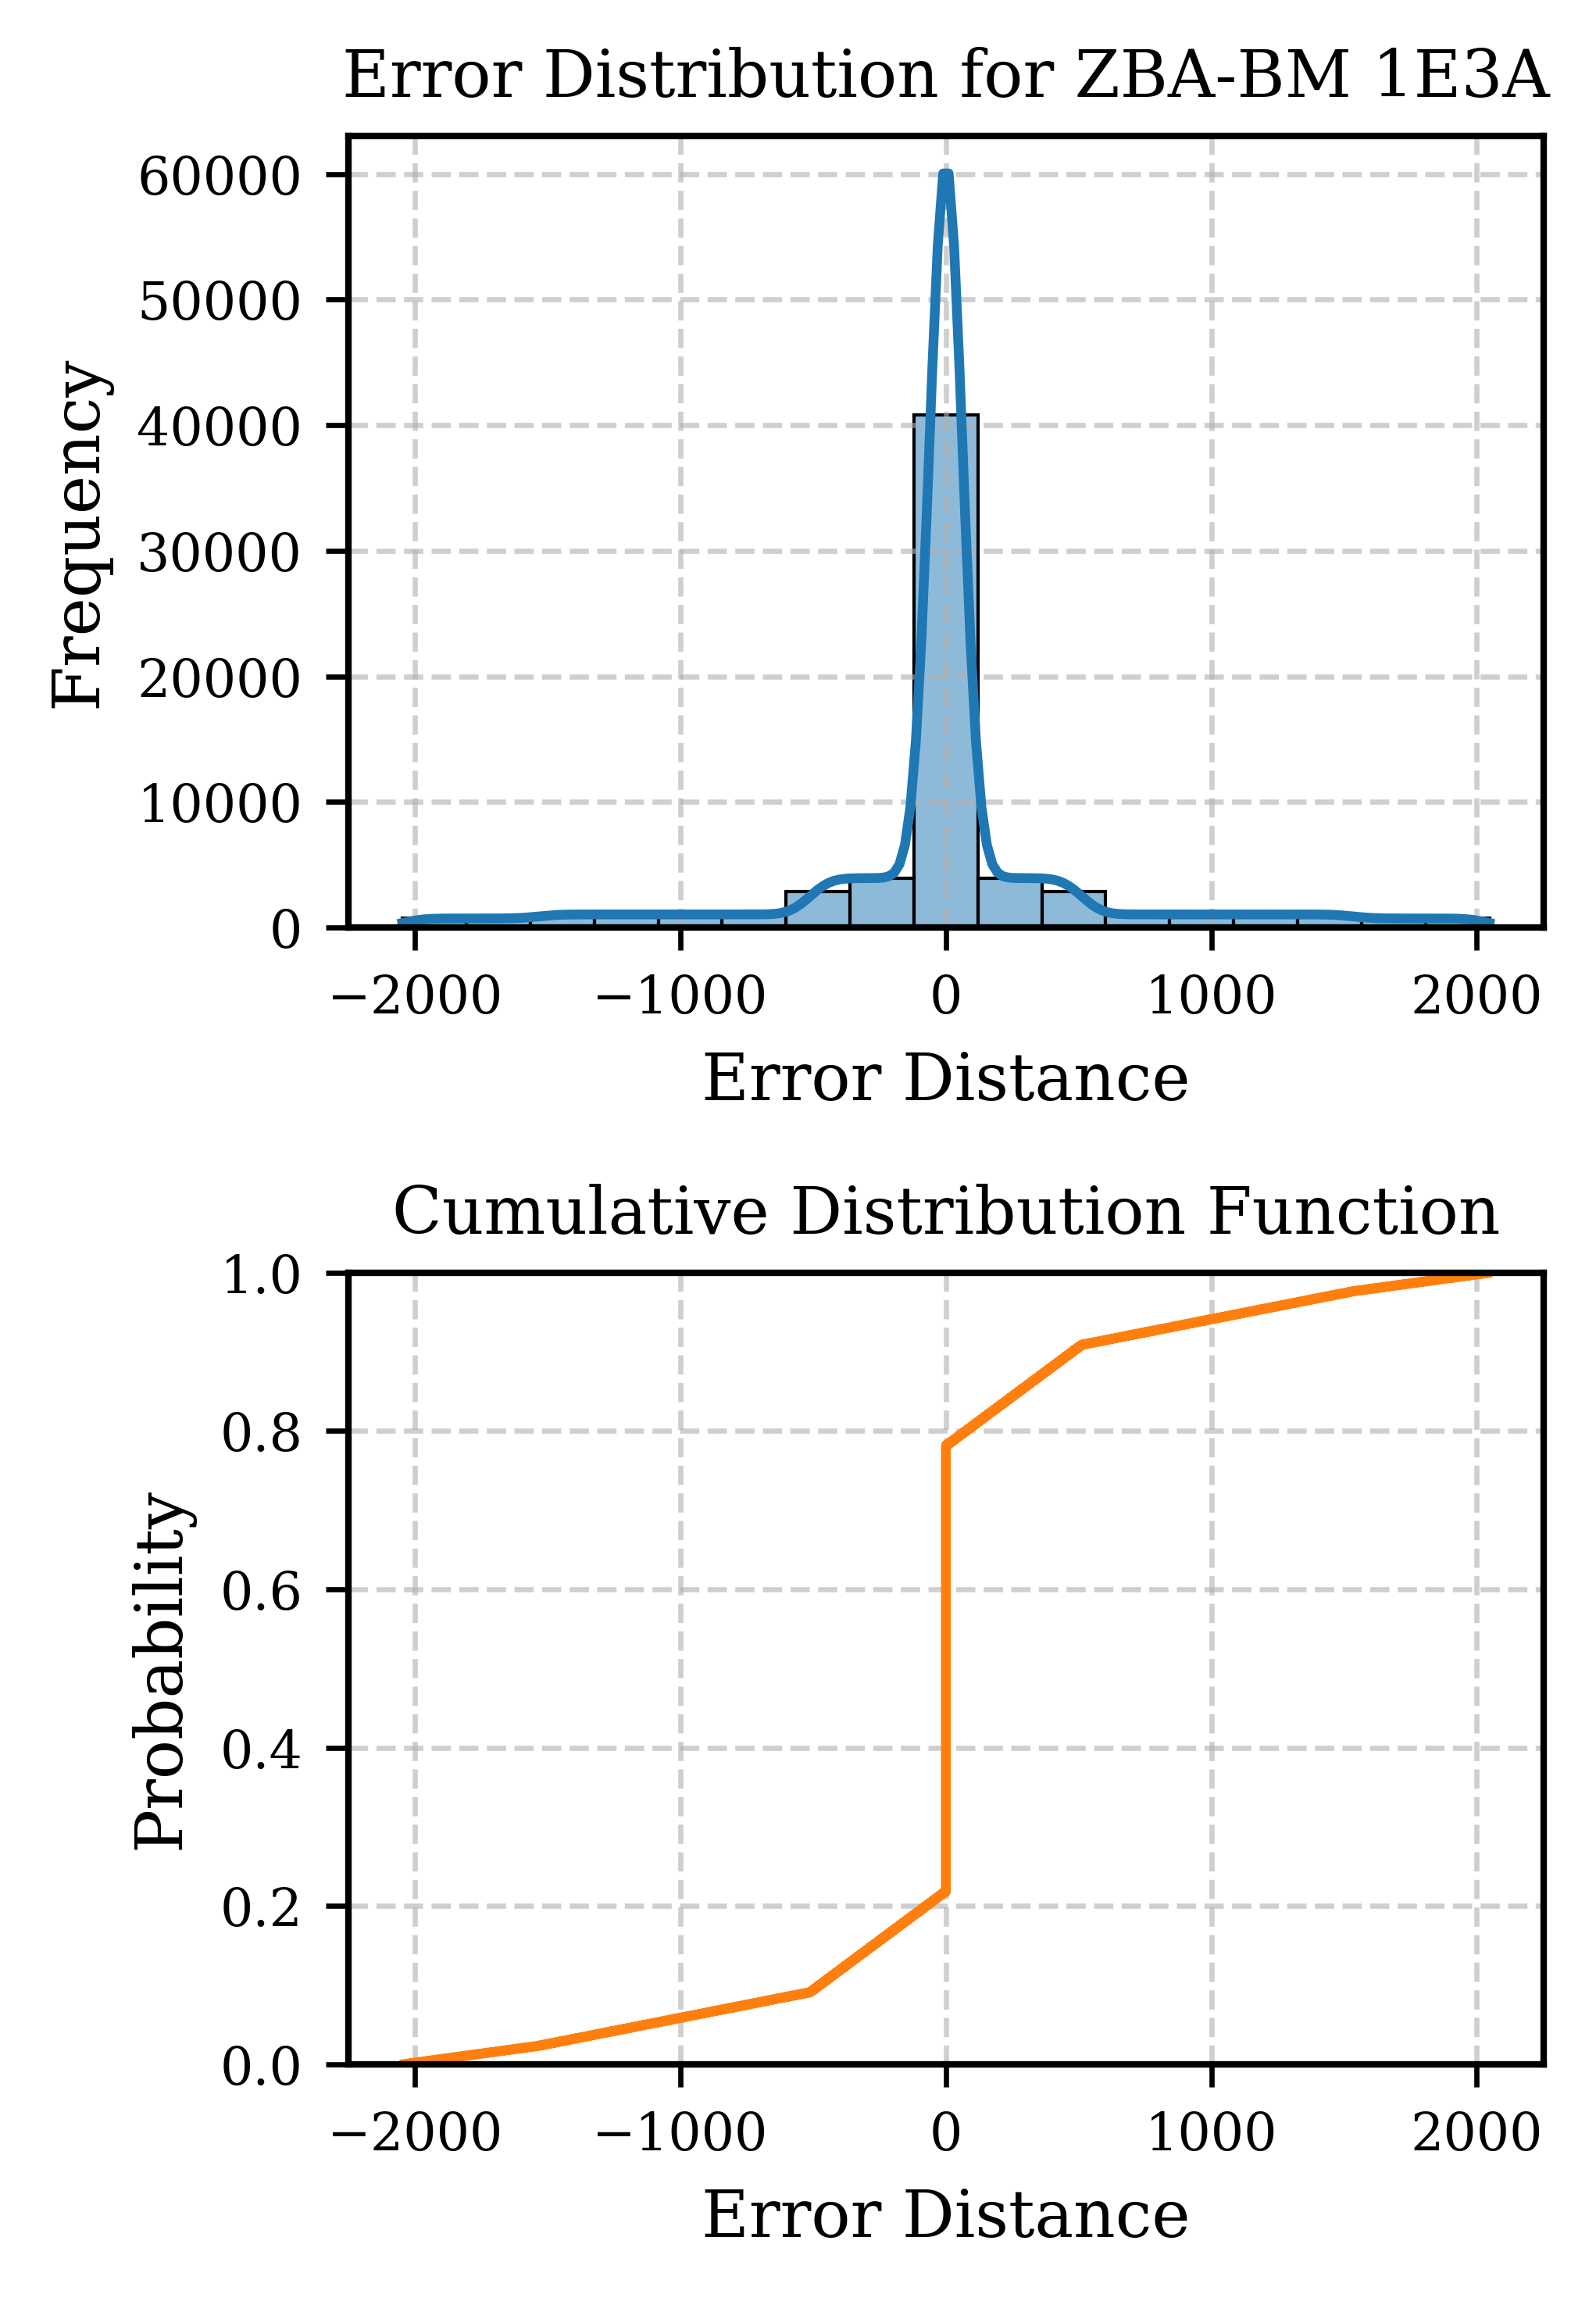
\includegraphics[width=\textwidth]{09_zbabm_1e3a_histogram.png}
        \caption{ZBA-BM 1E3A}
    \end{subfigure}\hfill
    \begin{subfigure}[b]{0.46\textwidth}
        \centering
        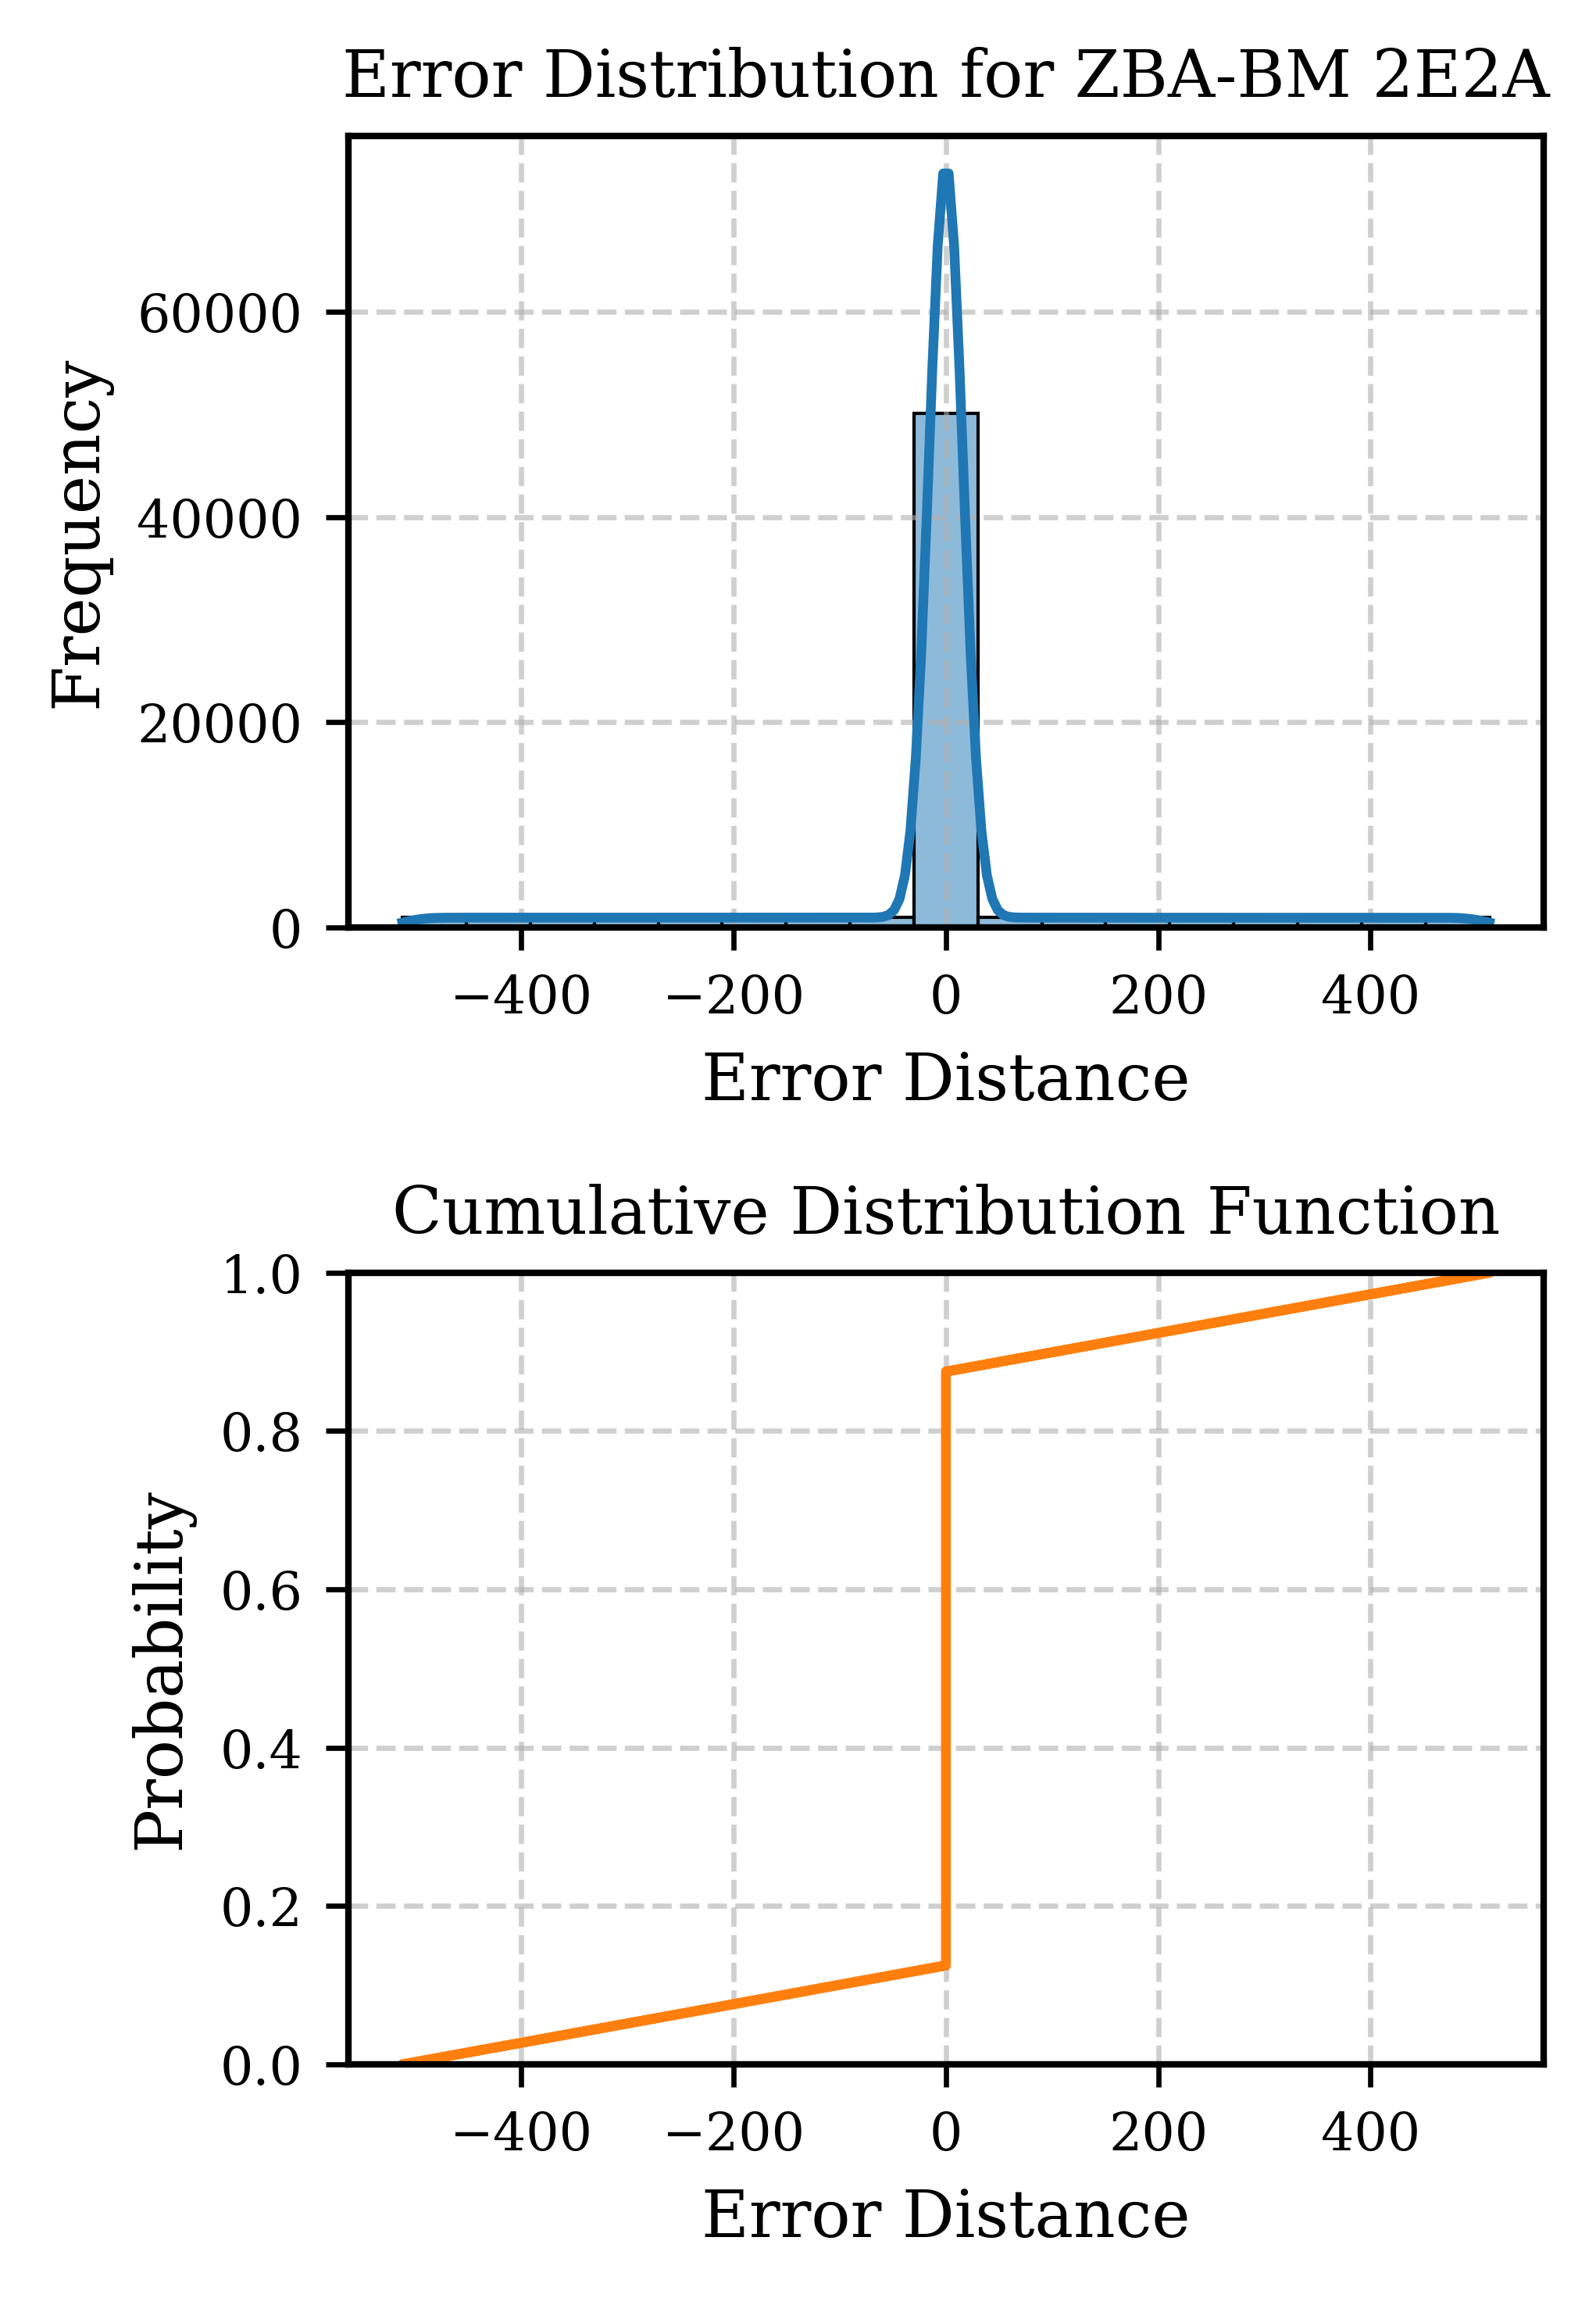
\includegraphics[width=\textwidth]{09_zbabm_2e2a_histogram.png}
        \caption{ZBA-BM 2E2A}
    \end{subfigure}
    \caption{四组 ZBA-BM 配置的误差直方图与经验累积分布对比}
    \label{fig:zbabm-hist-grid}
\end{figure}

\begin{figure}[H]
    \centering
    \begin{subfigure}[b]{0.46\textwidth}
        \centering
        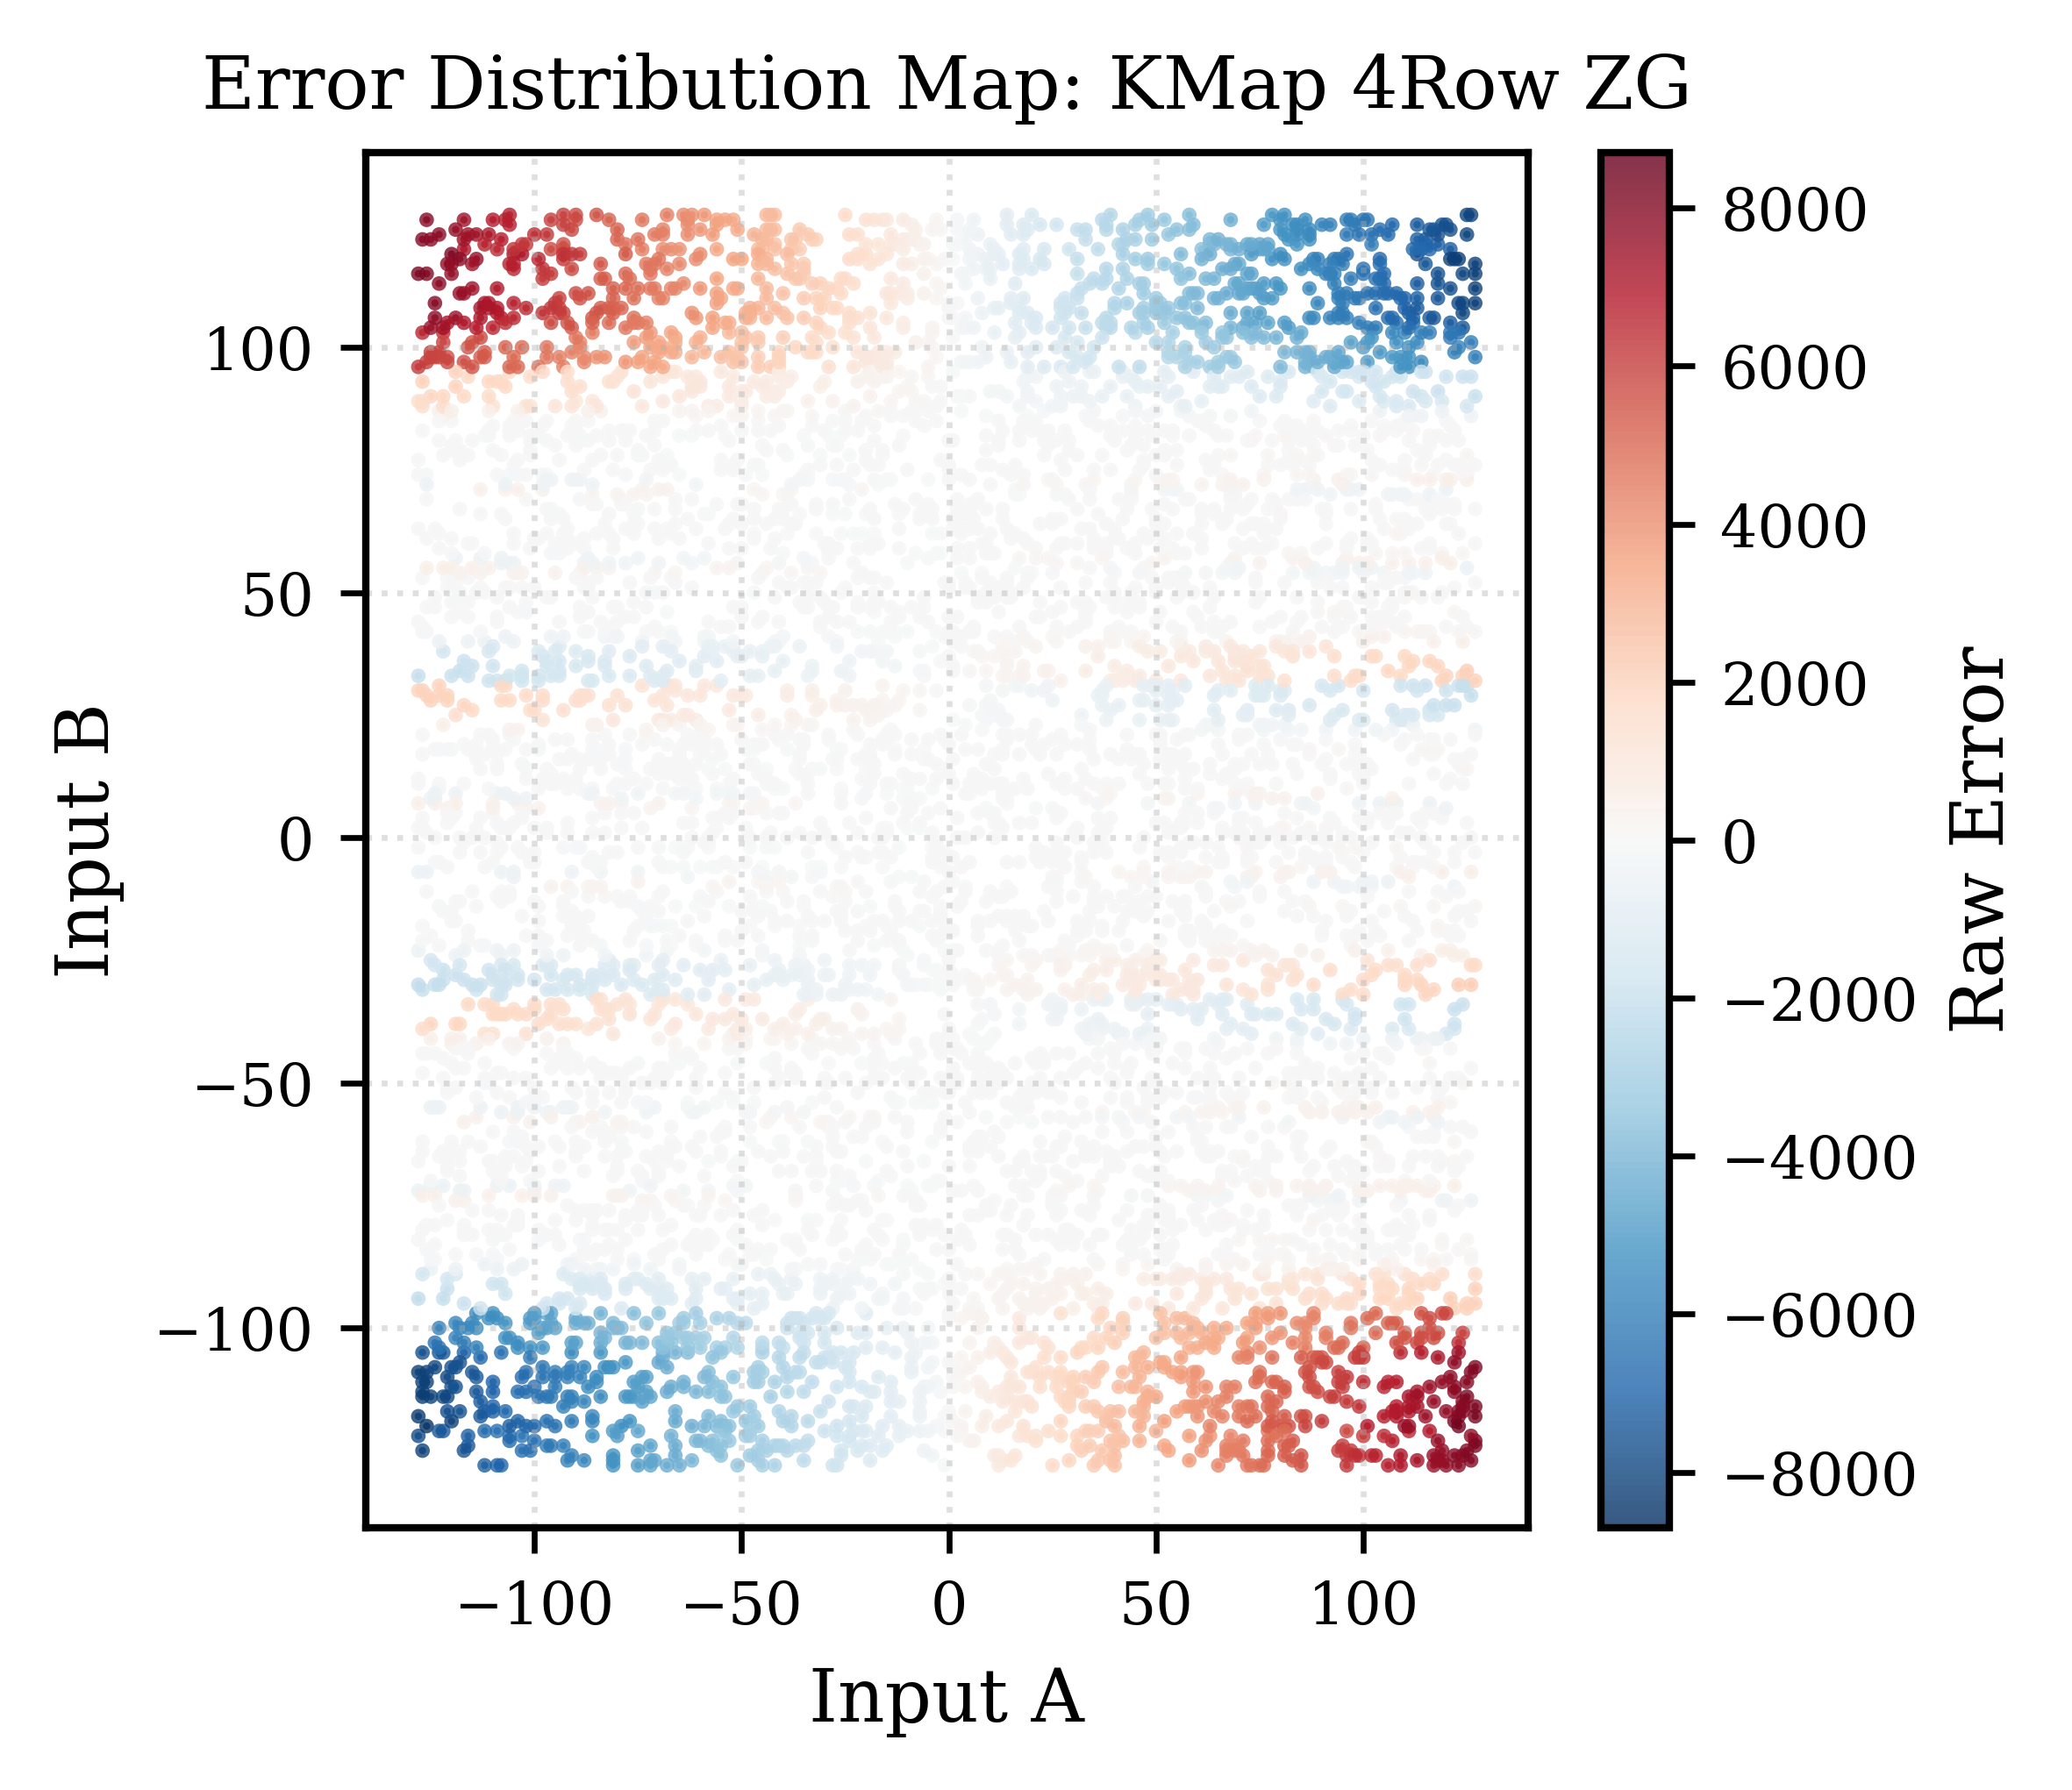
\includegraphics[width=\textwidth]{09_zbabm_4row_zg_heatmap.png}
        \caption{\texttt{KMap\_4Row\_ZG}}
    \end{subfigure}\hfill
    \begin{subfigure}[b]{0.46\textwidth}
        \centering
        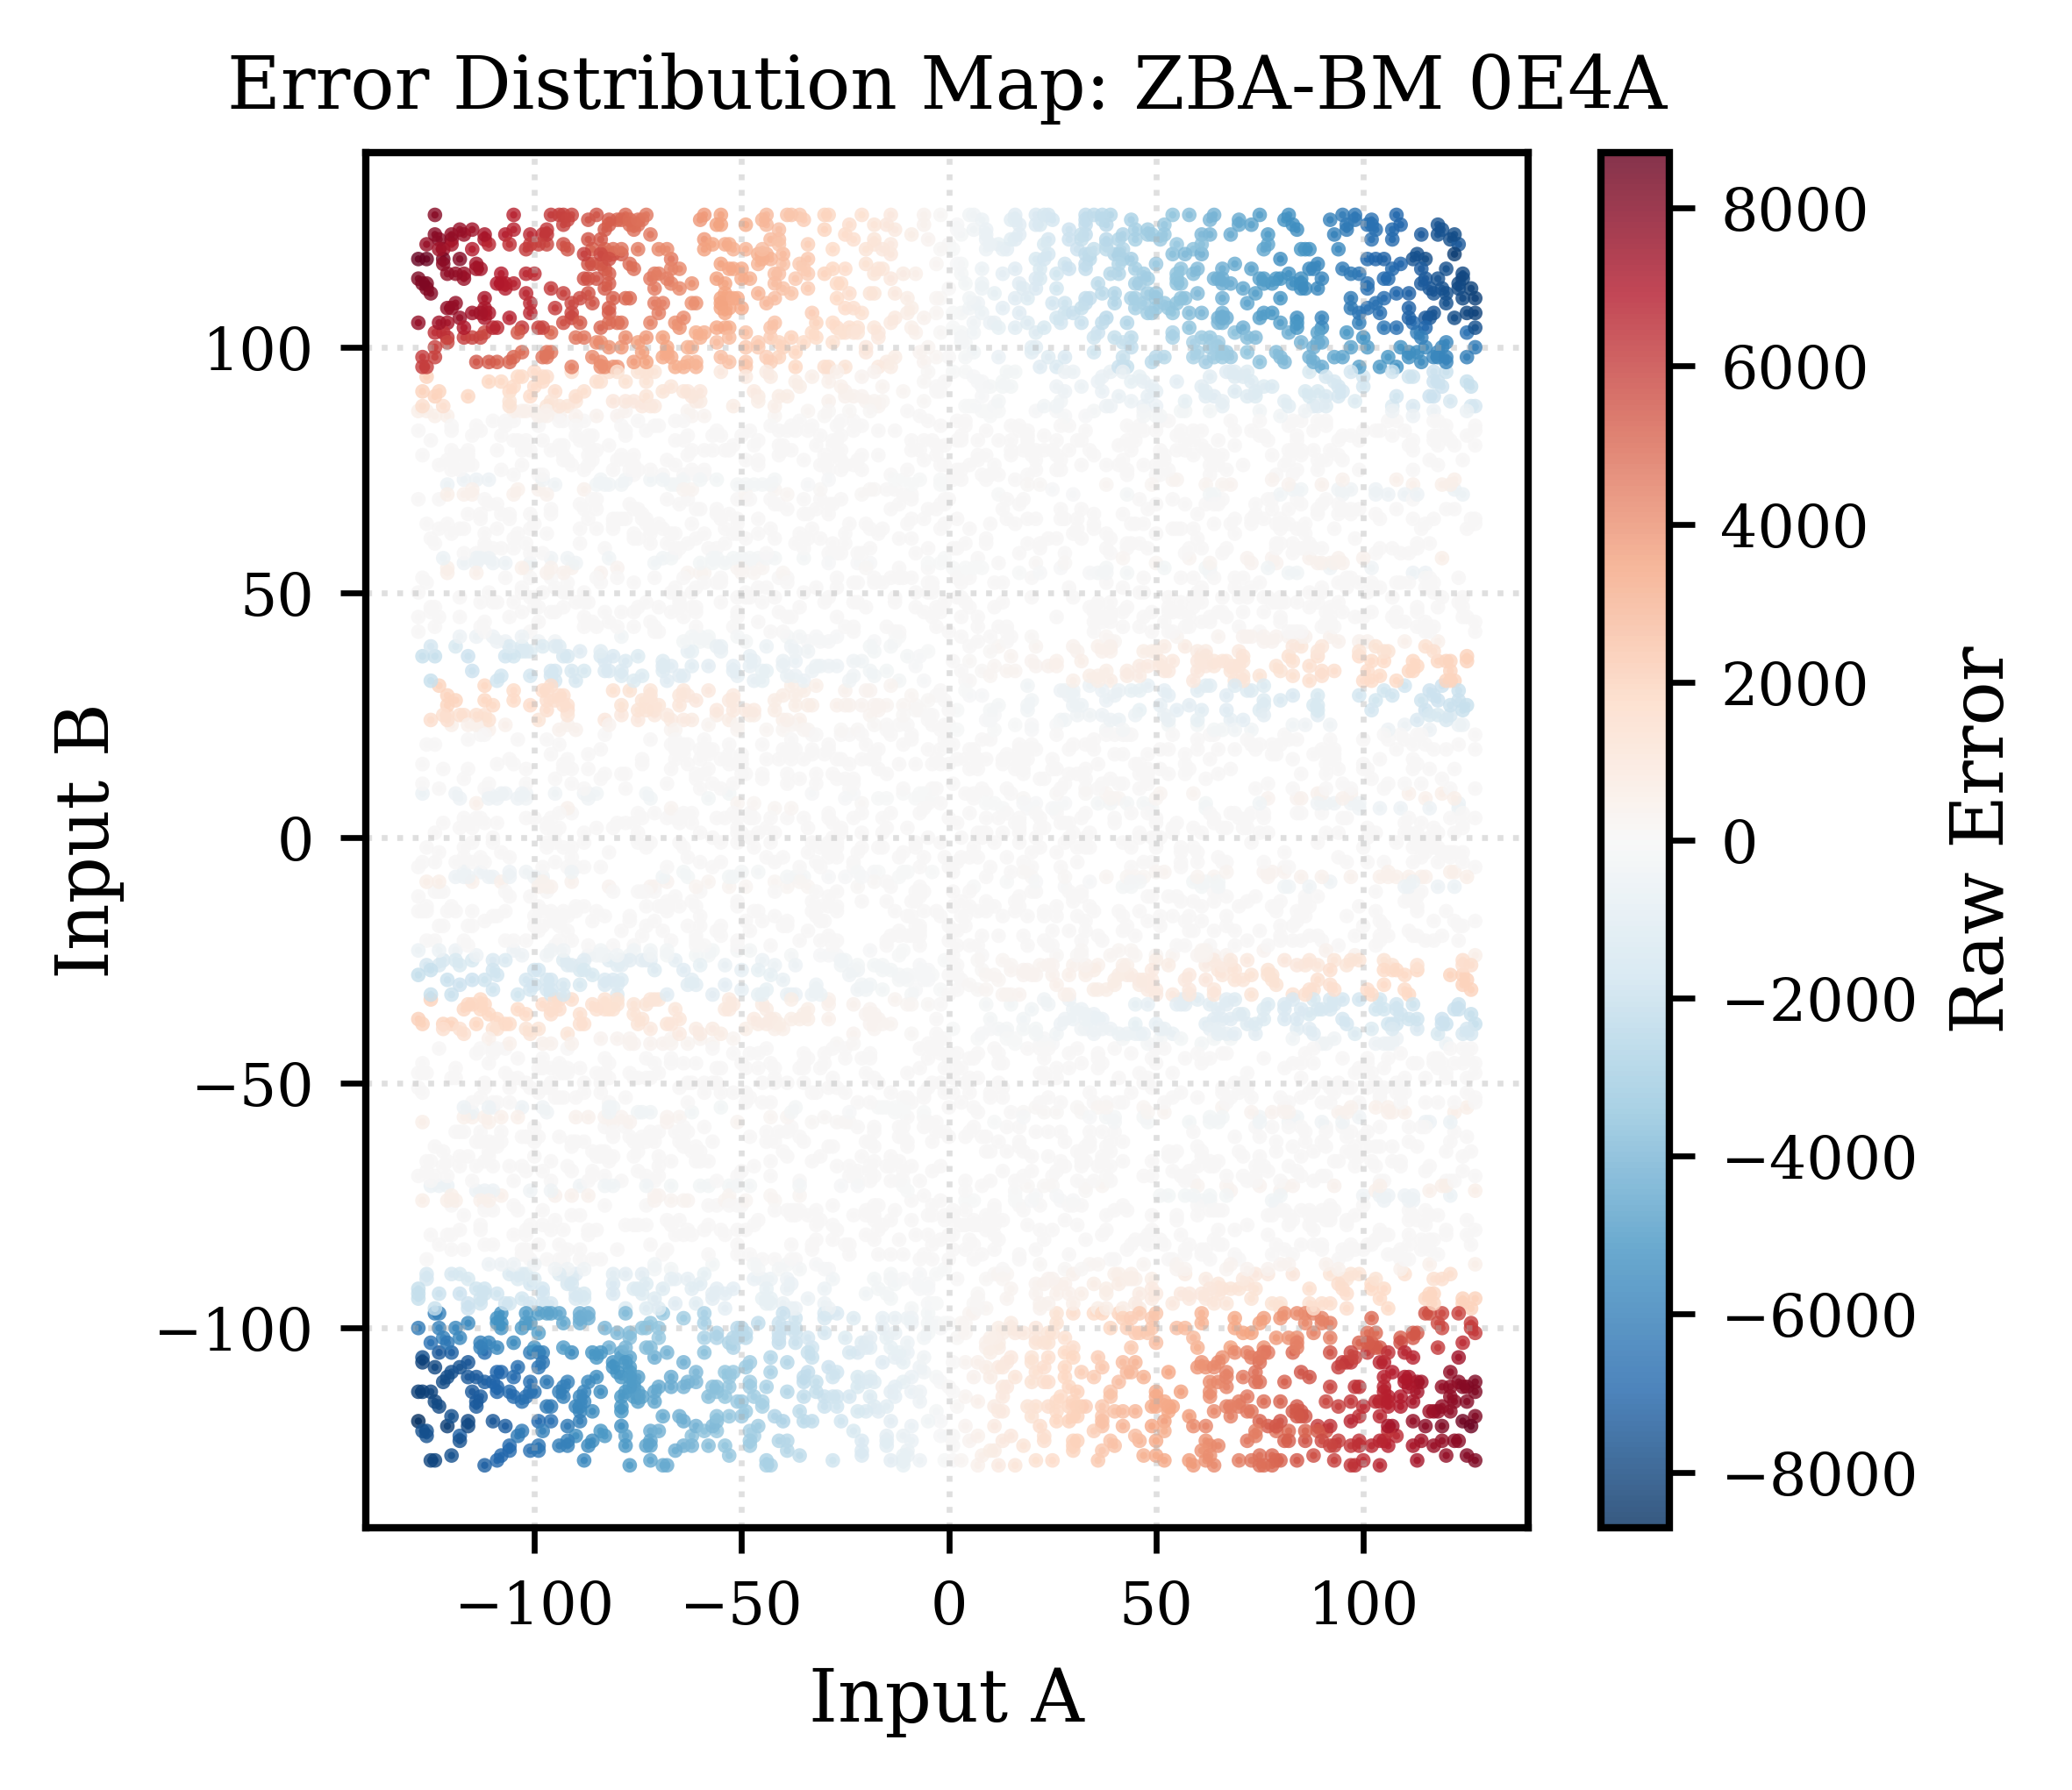
\includegraphics[width=\textwidth]{09_zbabm_0e4a_heatmap.png}
        \caption{ZBA-BM 0E4A}
    \end{subfigure}

    \vspace{0.2em}

    \begin{subfigure}[b]{0.46\textwidth}
        \centering
        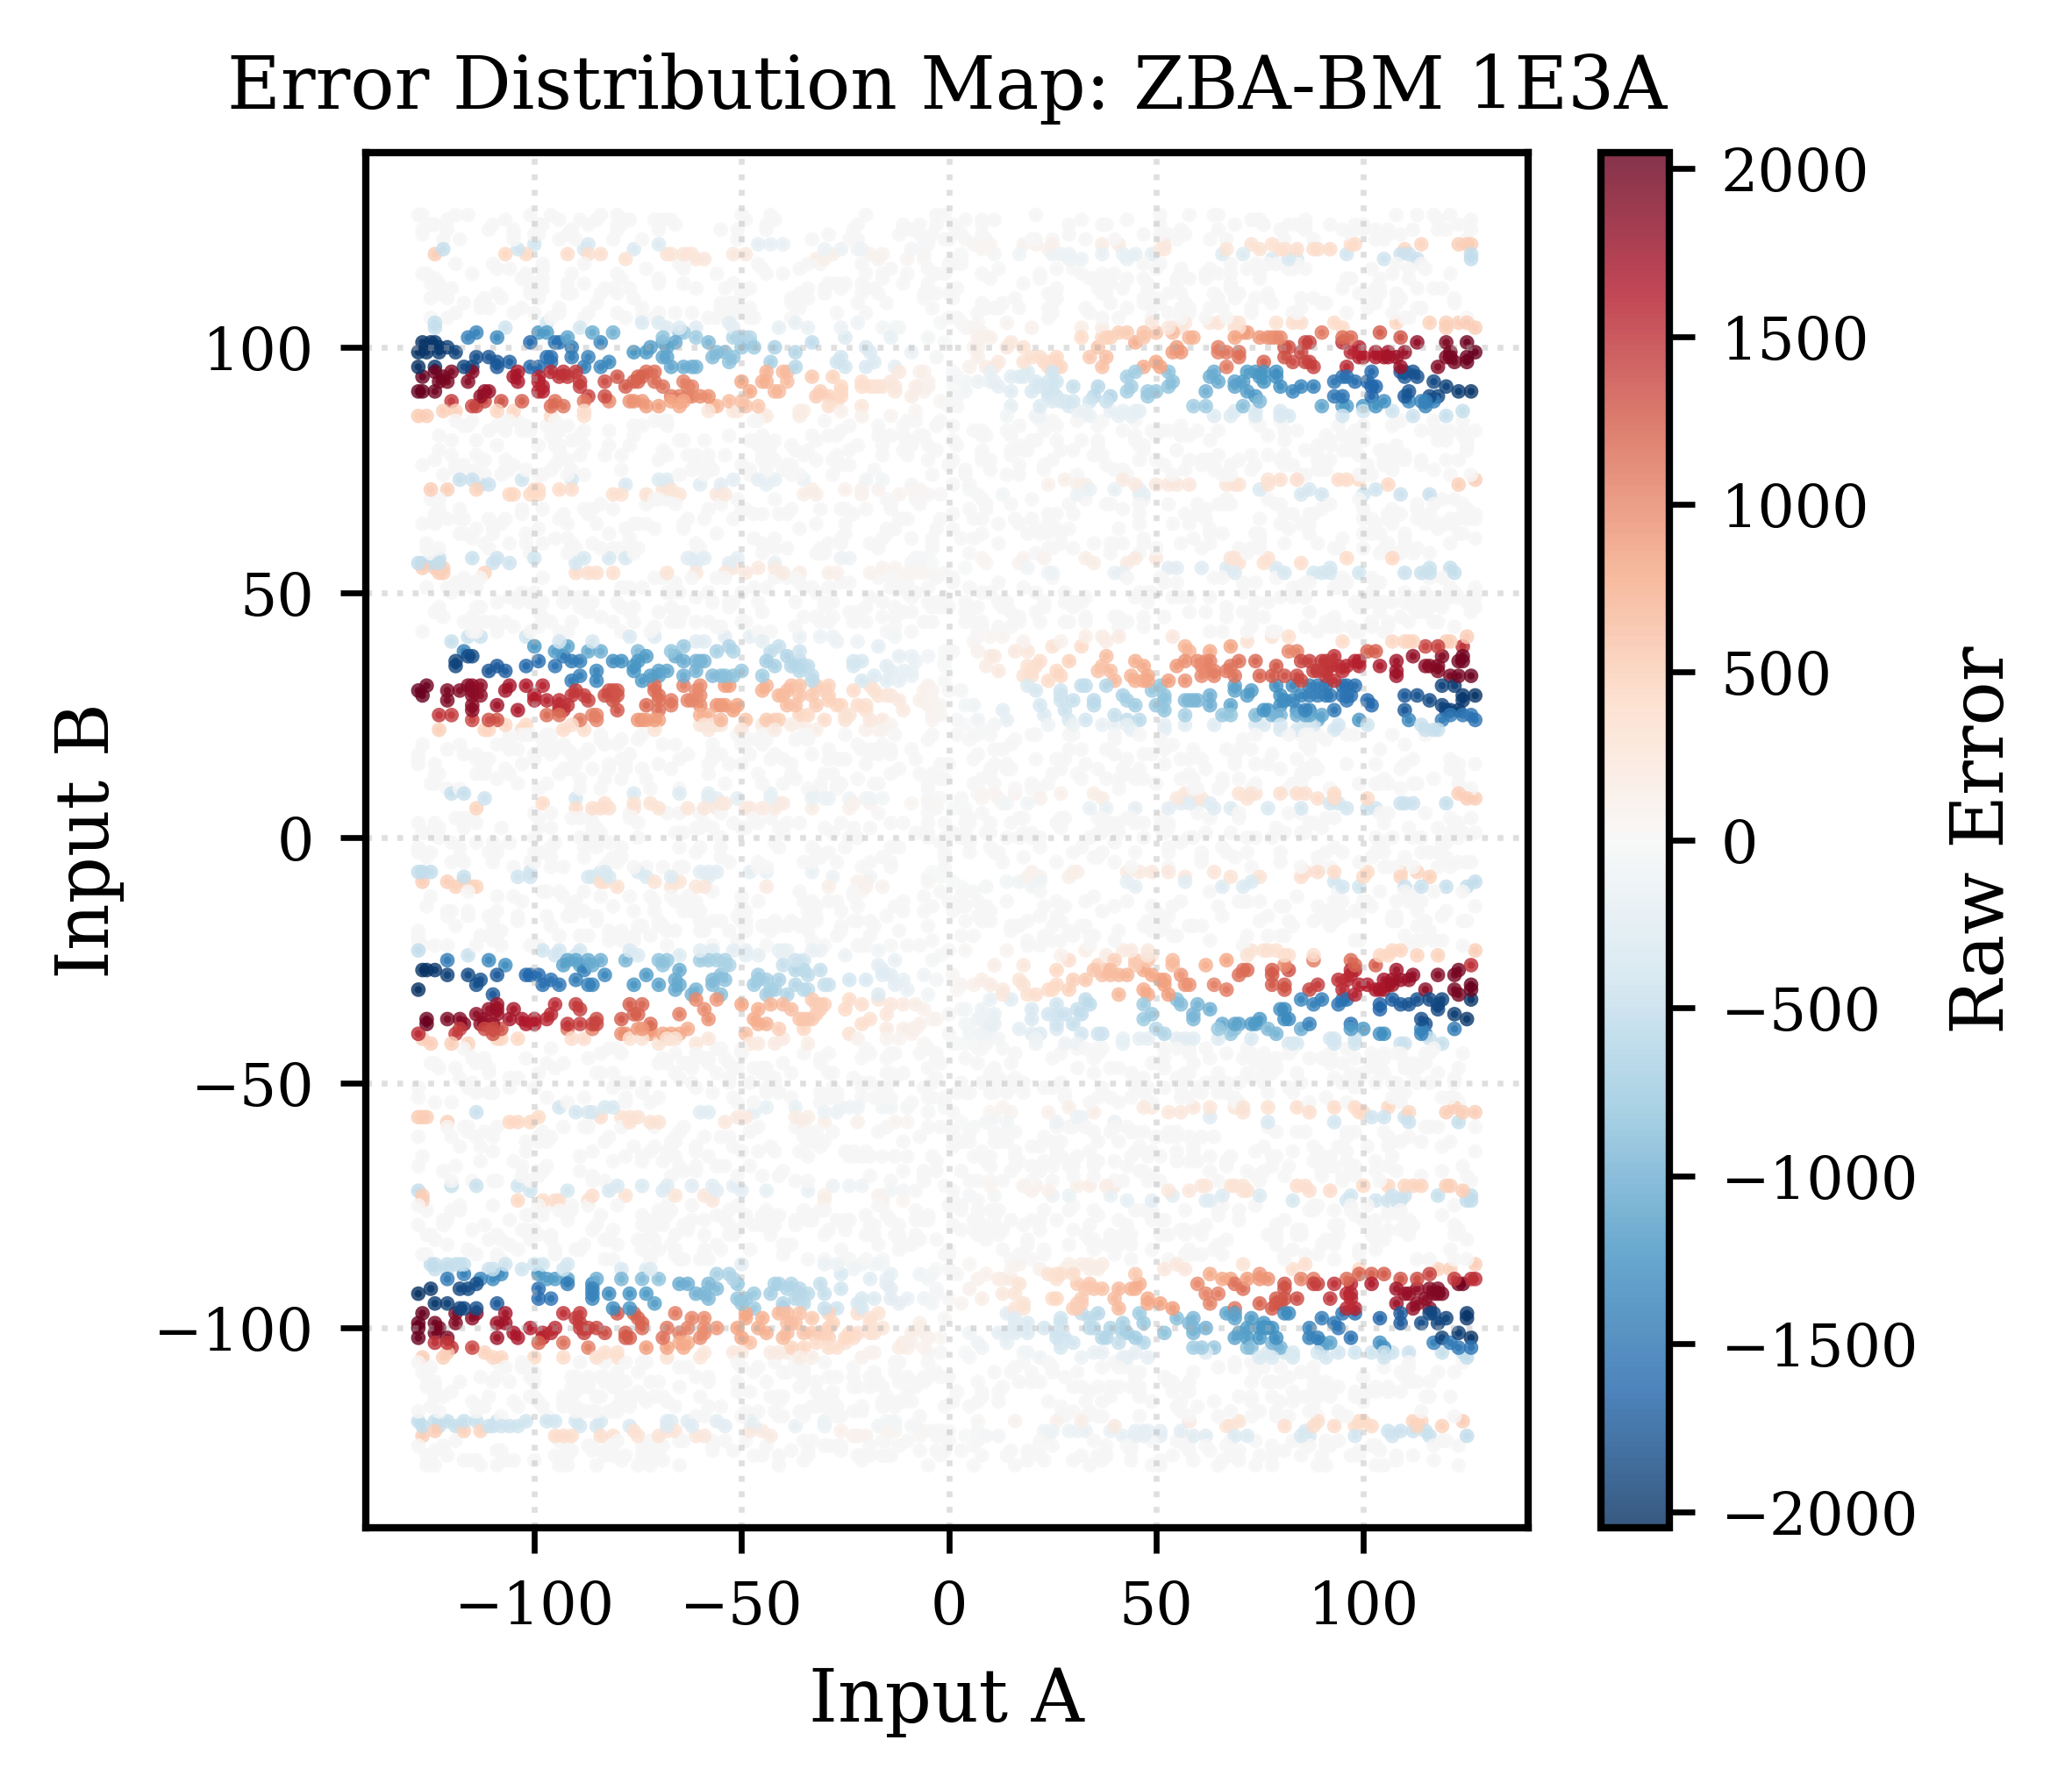
\includegraphics[width=\textwidth]{09_zbabm_1e3a_heatmap.png}
        \caption{ZBA-BM 1E3A}
    \end{subfigure}\hfill
    \begin{subfigure}[b]{0.46\textwidth}
        \centering
        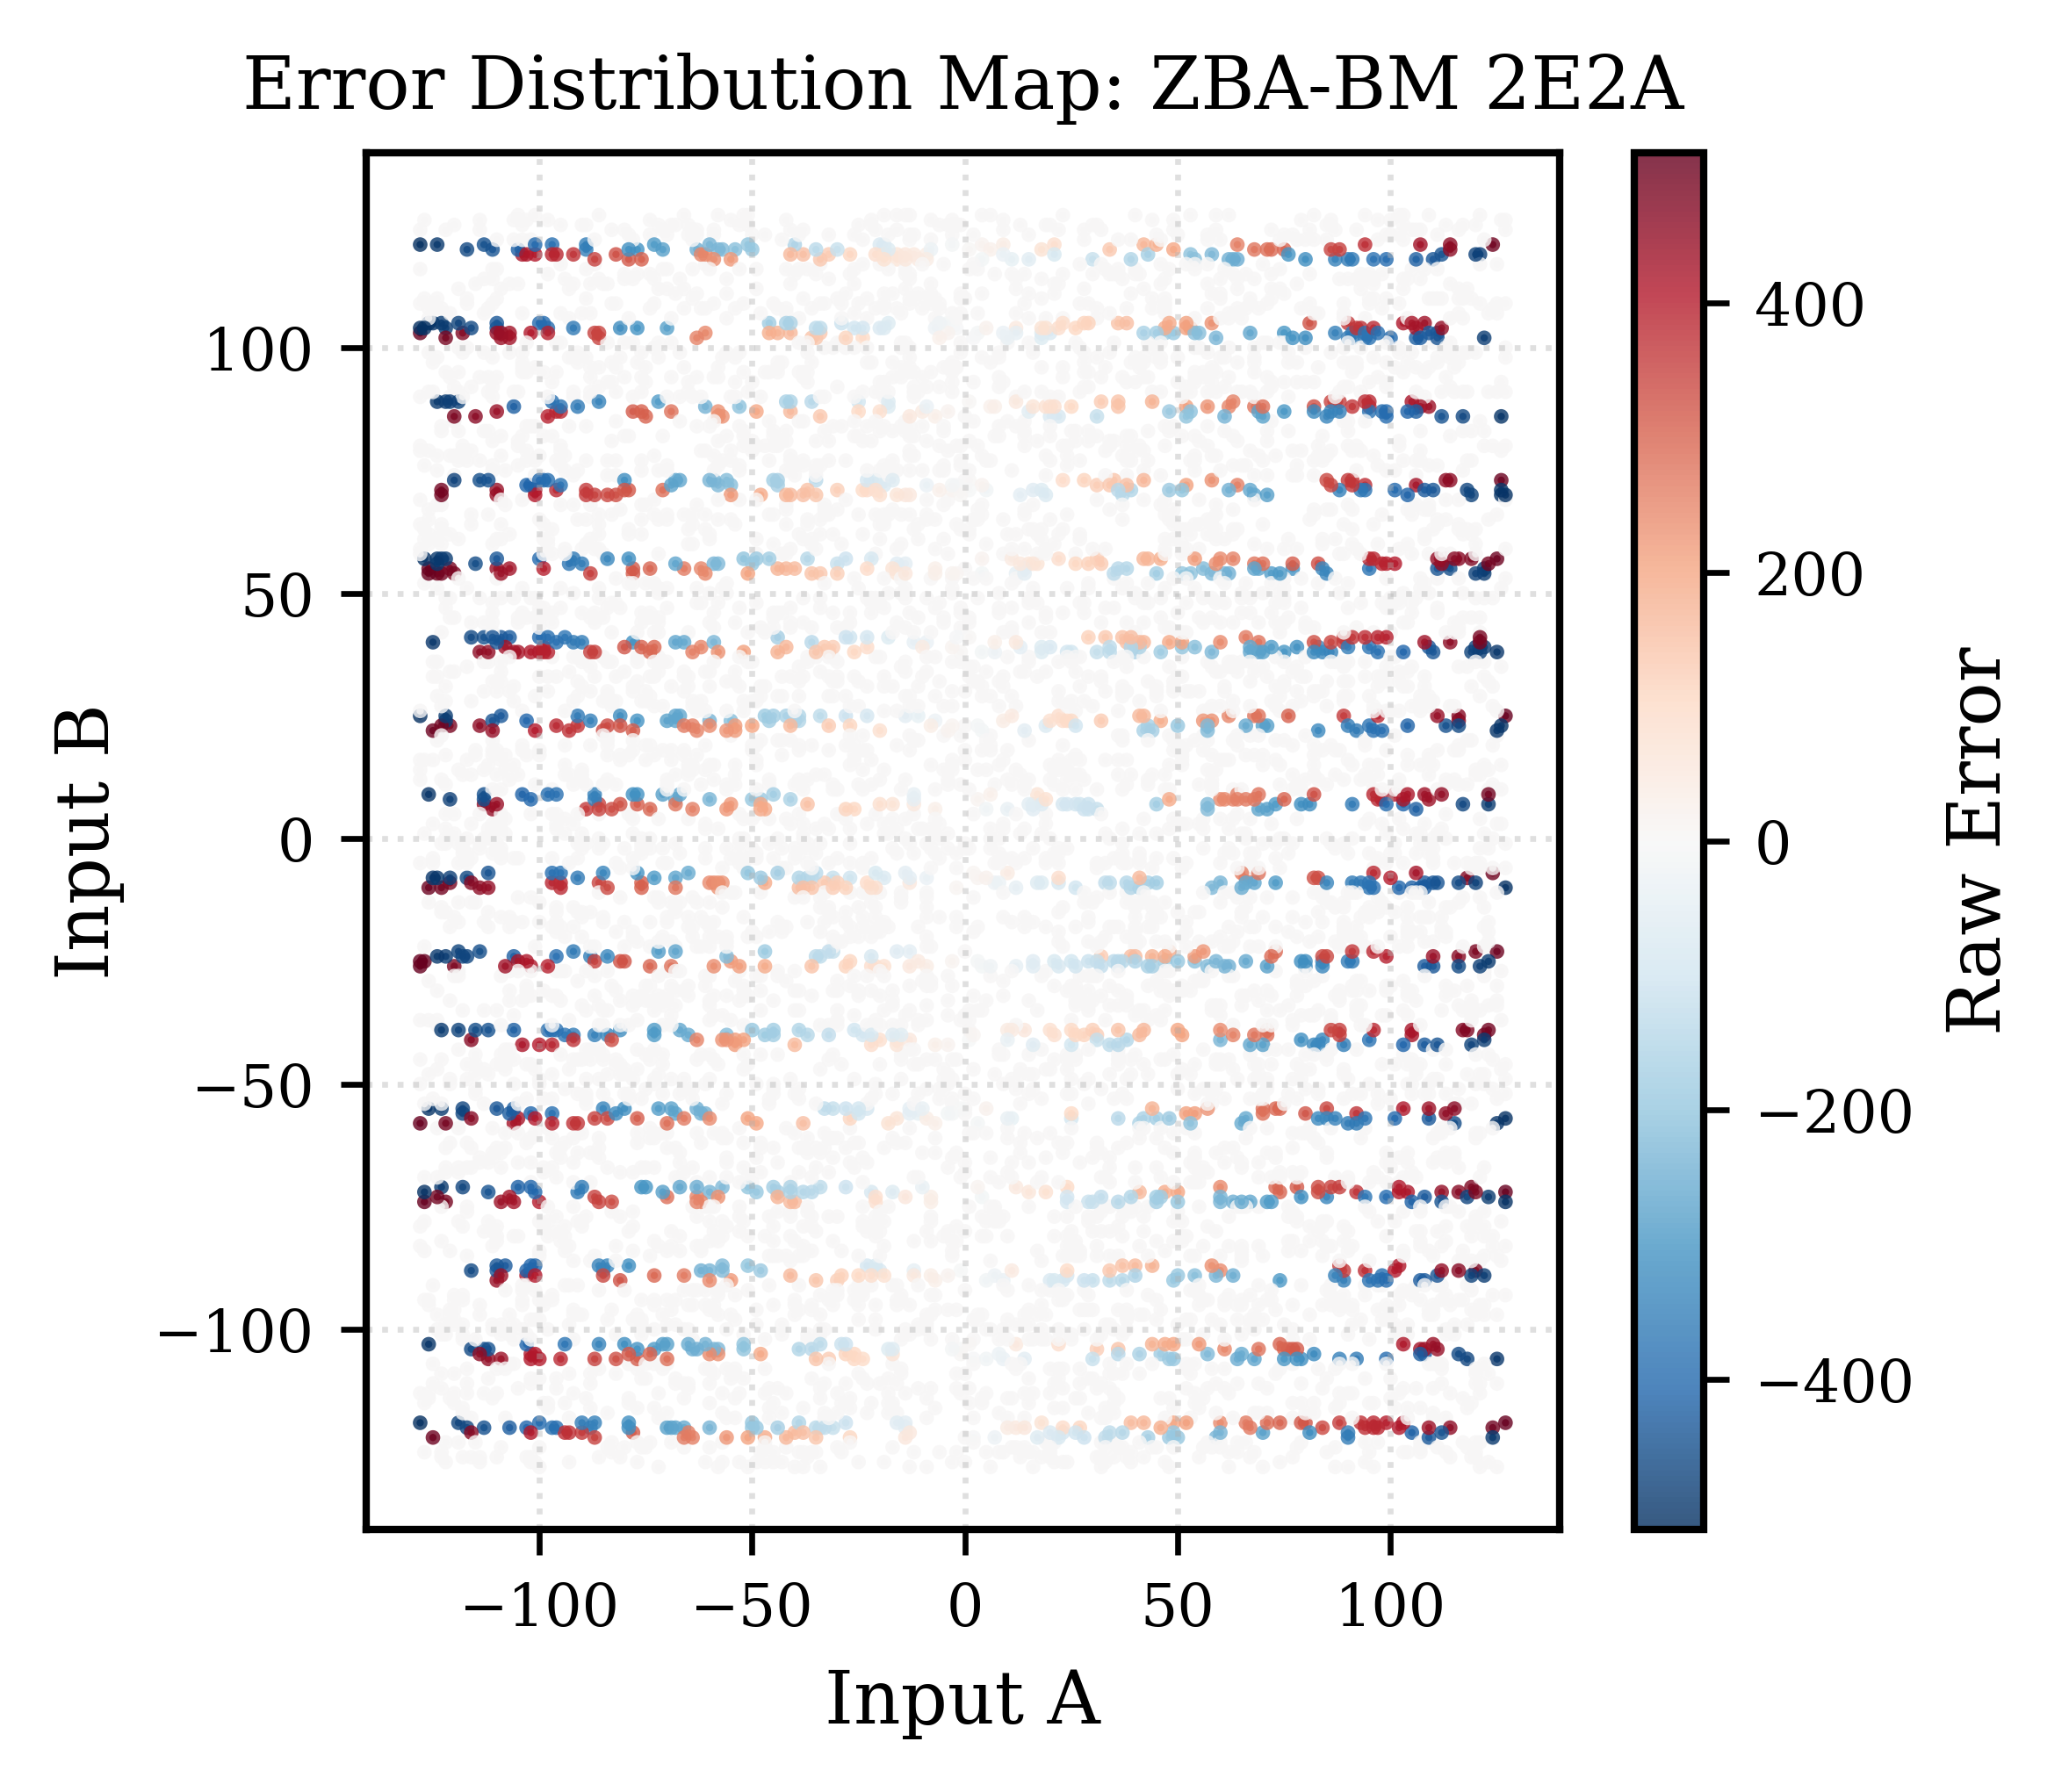
\includegraphics[width=\textwidth]{09_zbabm_2e2a_heatmap.png}
        \caption{ZBA-BM 2E2A}
    \end{subfigure}
    \caption{四组 ZBA-BM 配置在输入空间上的误差分布热力图对比}
    \label{fig:zbabm-heat-grid}
\end{figure}

\clearpage
\subsubsection{LETAM 近似乘法器的误差分析}

为了评估LETAM算法的算子级误差特性，本文针对8位有符号乘法全区间（共65536组测试用例）进行仿真遍历，对比了四组代表性配置的具体偏差分布。表\ref{tab:letam_error}展示了全局误差统计结果。

\begin{table}[htbp]
\centering
\caption{LETAM 不同参数配置的全遍历误差统计对比}
\label{tab:letam_error}
\begin{tabular}{lcccccccc}
\toprule
\textbf{指标} & \textbf{LETAM(2,4)} & \textbf{LETAM(3,6)} & \textbf{LETAM(3,8)} & \textbf{LETAM(4,8)} \\
\midrule
ME            & $-0.52$   & $-0.31$   & $-0.18$   & $-0.09$   \\
MAE           & 197.00    & 107.00    & 72.00     & 51.00     \\
RMSE          & 349.00    & 207.00    & 143.00    & 102.00    \\
MARE(\%)      & 5.16      & 2.74      & 1.85      & 1.30      \\
MRED(\%)      & 5.08      & 2.71      & 1.83      & 1.29      \\
NMED          & 6.04      & 3.28      & 2.21      & 1.56      \\
Sign Errors   & 48        & 20        & 12        & 8         \\
\bottomrule
\end{tabular}
\end{table}

实验结果表明，LETAM的误差分布呈现高度可控与快速收敛的特征。各项误差随内部保留参数提升显著降低；例如从LETAM(2,4)至LETAM(4,8)，平均绝对误差（MAE）下降74.1\%。各配置极小的负均值（ME）表明，内部位级截断仅引发微弱且易向零点弥散的欠估计。在关键参数影响上，加法项保留位宽$TP$占据主导地位：固定乘法项$T=3$时，将$TP$由6提升至8可使MAE下降32.7\%，效果优于单纯提升$T$位宽。此外，全组态的符号翻转样本率均低于0.07\%，体现出优异的极端算值符号保真度。综合硬件开销估算，LETAM(3,6)配置以36位宽的操作核达成了2.74\%的极低平均相对误差（MARE），在精度与面积象限间实现了最佳权衡，将其定为理论推荐基准。

图\ref{fig:letam_hist_cdf}的绝对误差频率直方图与累积分布函数（CDF）表明，全系配置的误差分布均呈右偏态，绝大多数偏差事件密集富集于极小区间（$|E| < 50$）内。相较于低精度配置的平缓发散，LETAM(4,8)配置呈现出锐利的直方图峰刺与最陡峭的CDF急变区。对于基准推荐配置LETAM(3,6)而言，75\%的应用误差被内生约束机制锁定在150以下，证实了其在常规算术场景中的低偏差长时间驻留属性。

\begin{figure}[htpb]
\centering
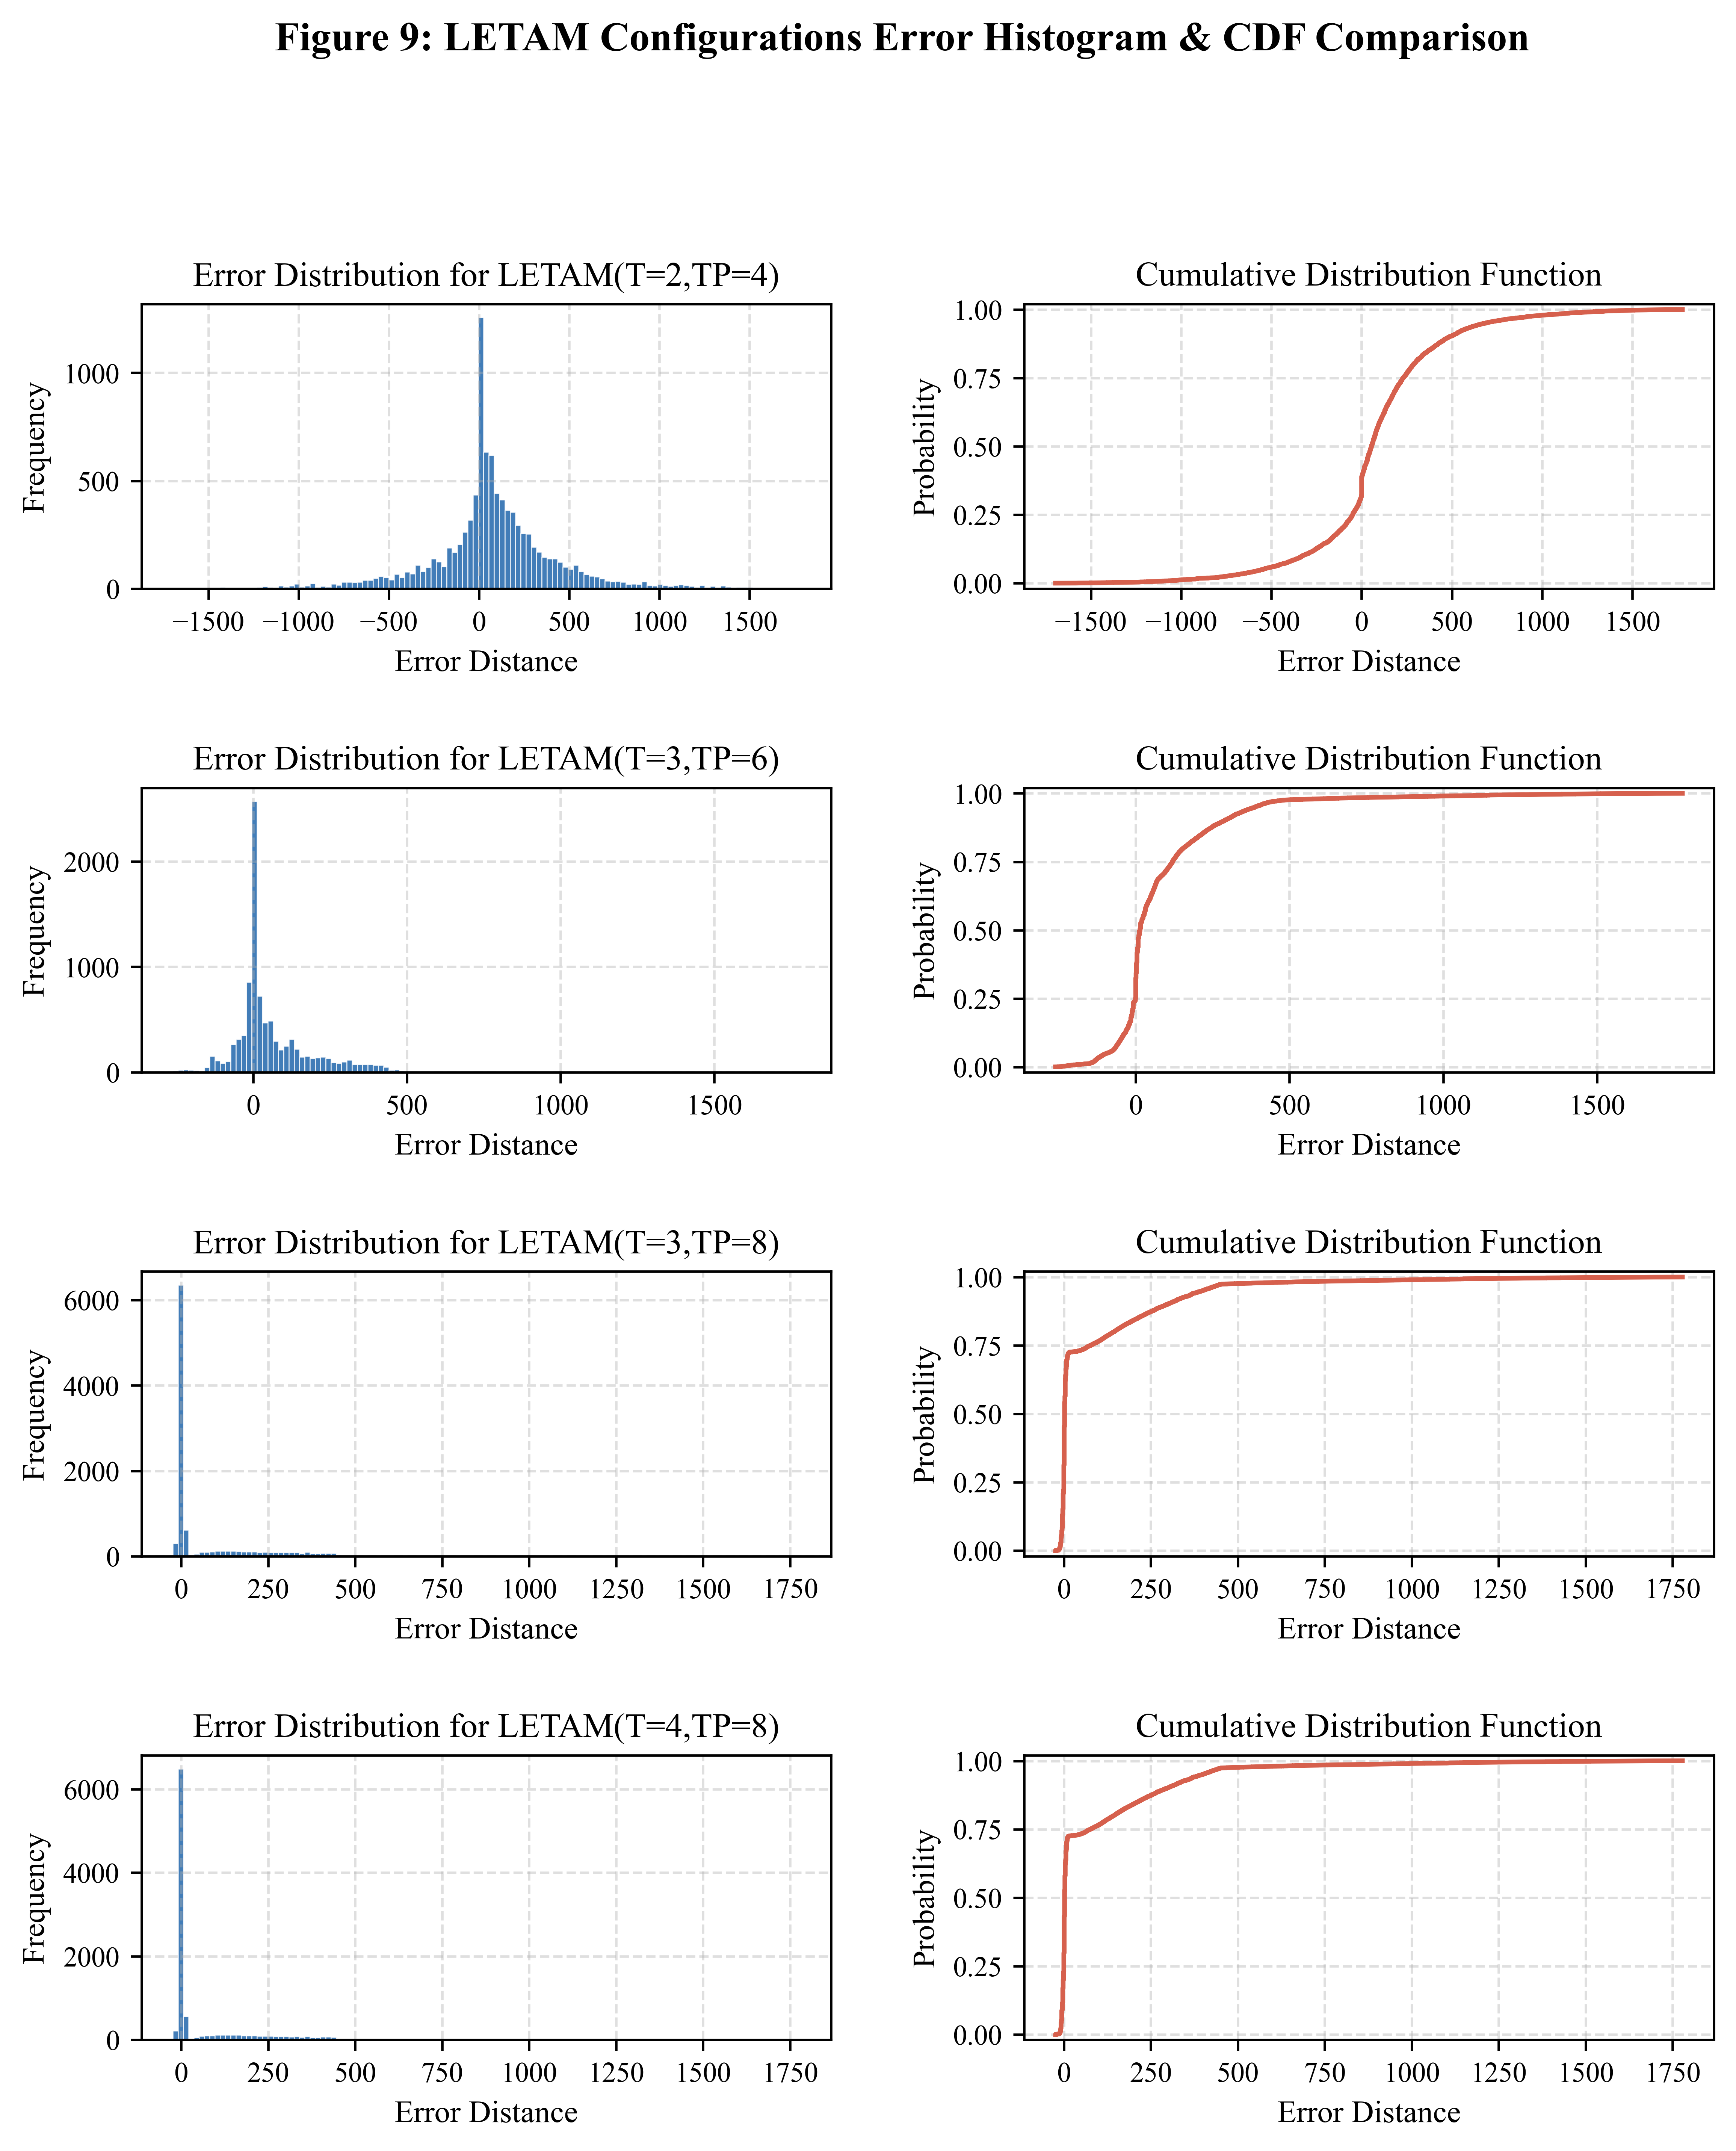
\includegraphics[width=0.95\textwidth]{LETAM_Fig9_histogram_cdf.png}
\caption{LETAM 多配置绝对误差直方图与累积分布函数}
\label{fig:letam_hist_cdf}
\end{figure}

图\ref{fig:letam_heatmap}以热力图展示了综合误差的二维输入映射关系，呈现出三项突出的空间规律。首先，沿坐标轴（$A \approx 0$或$B \approx 0$）附近弥散有带状高误差积聚，这是由于微小计算数前导一索引骤降，导致移频重构机制补偿受限；其次，一、三象限（同号乘法）区域误差明显低于二、四象限（异号乘法），这种非对称性源于底层算术单元对异符号计算采取的妥协性缩放补偿增益；最后，在两界坐标满偏极值区域（$|A|,|B| \to 128$），先序尾码截断的伴生偏差在极端条件下面临了指数级补偿放大的关联扩展，不可避免地诱发了局部点斑状极值现象。

\begin{figure}[htpb]
\centering
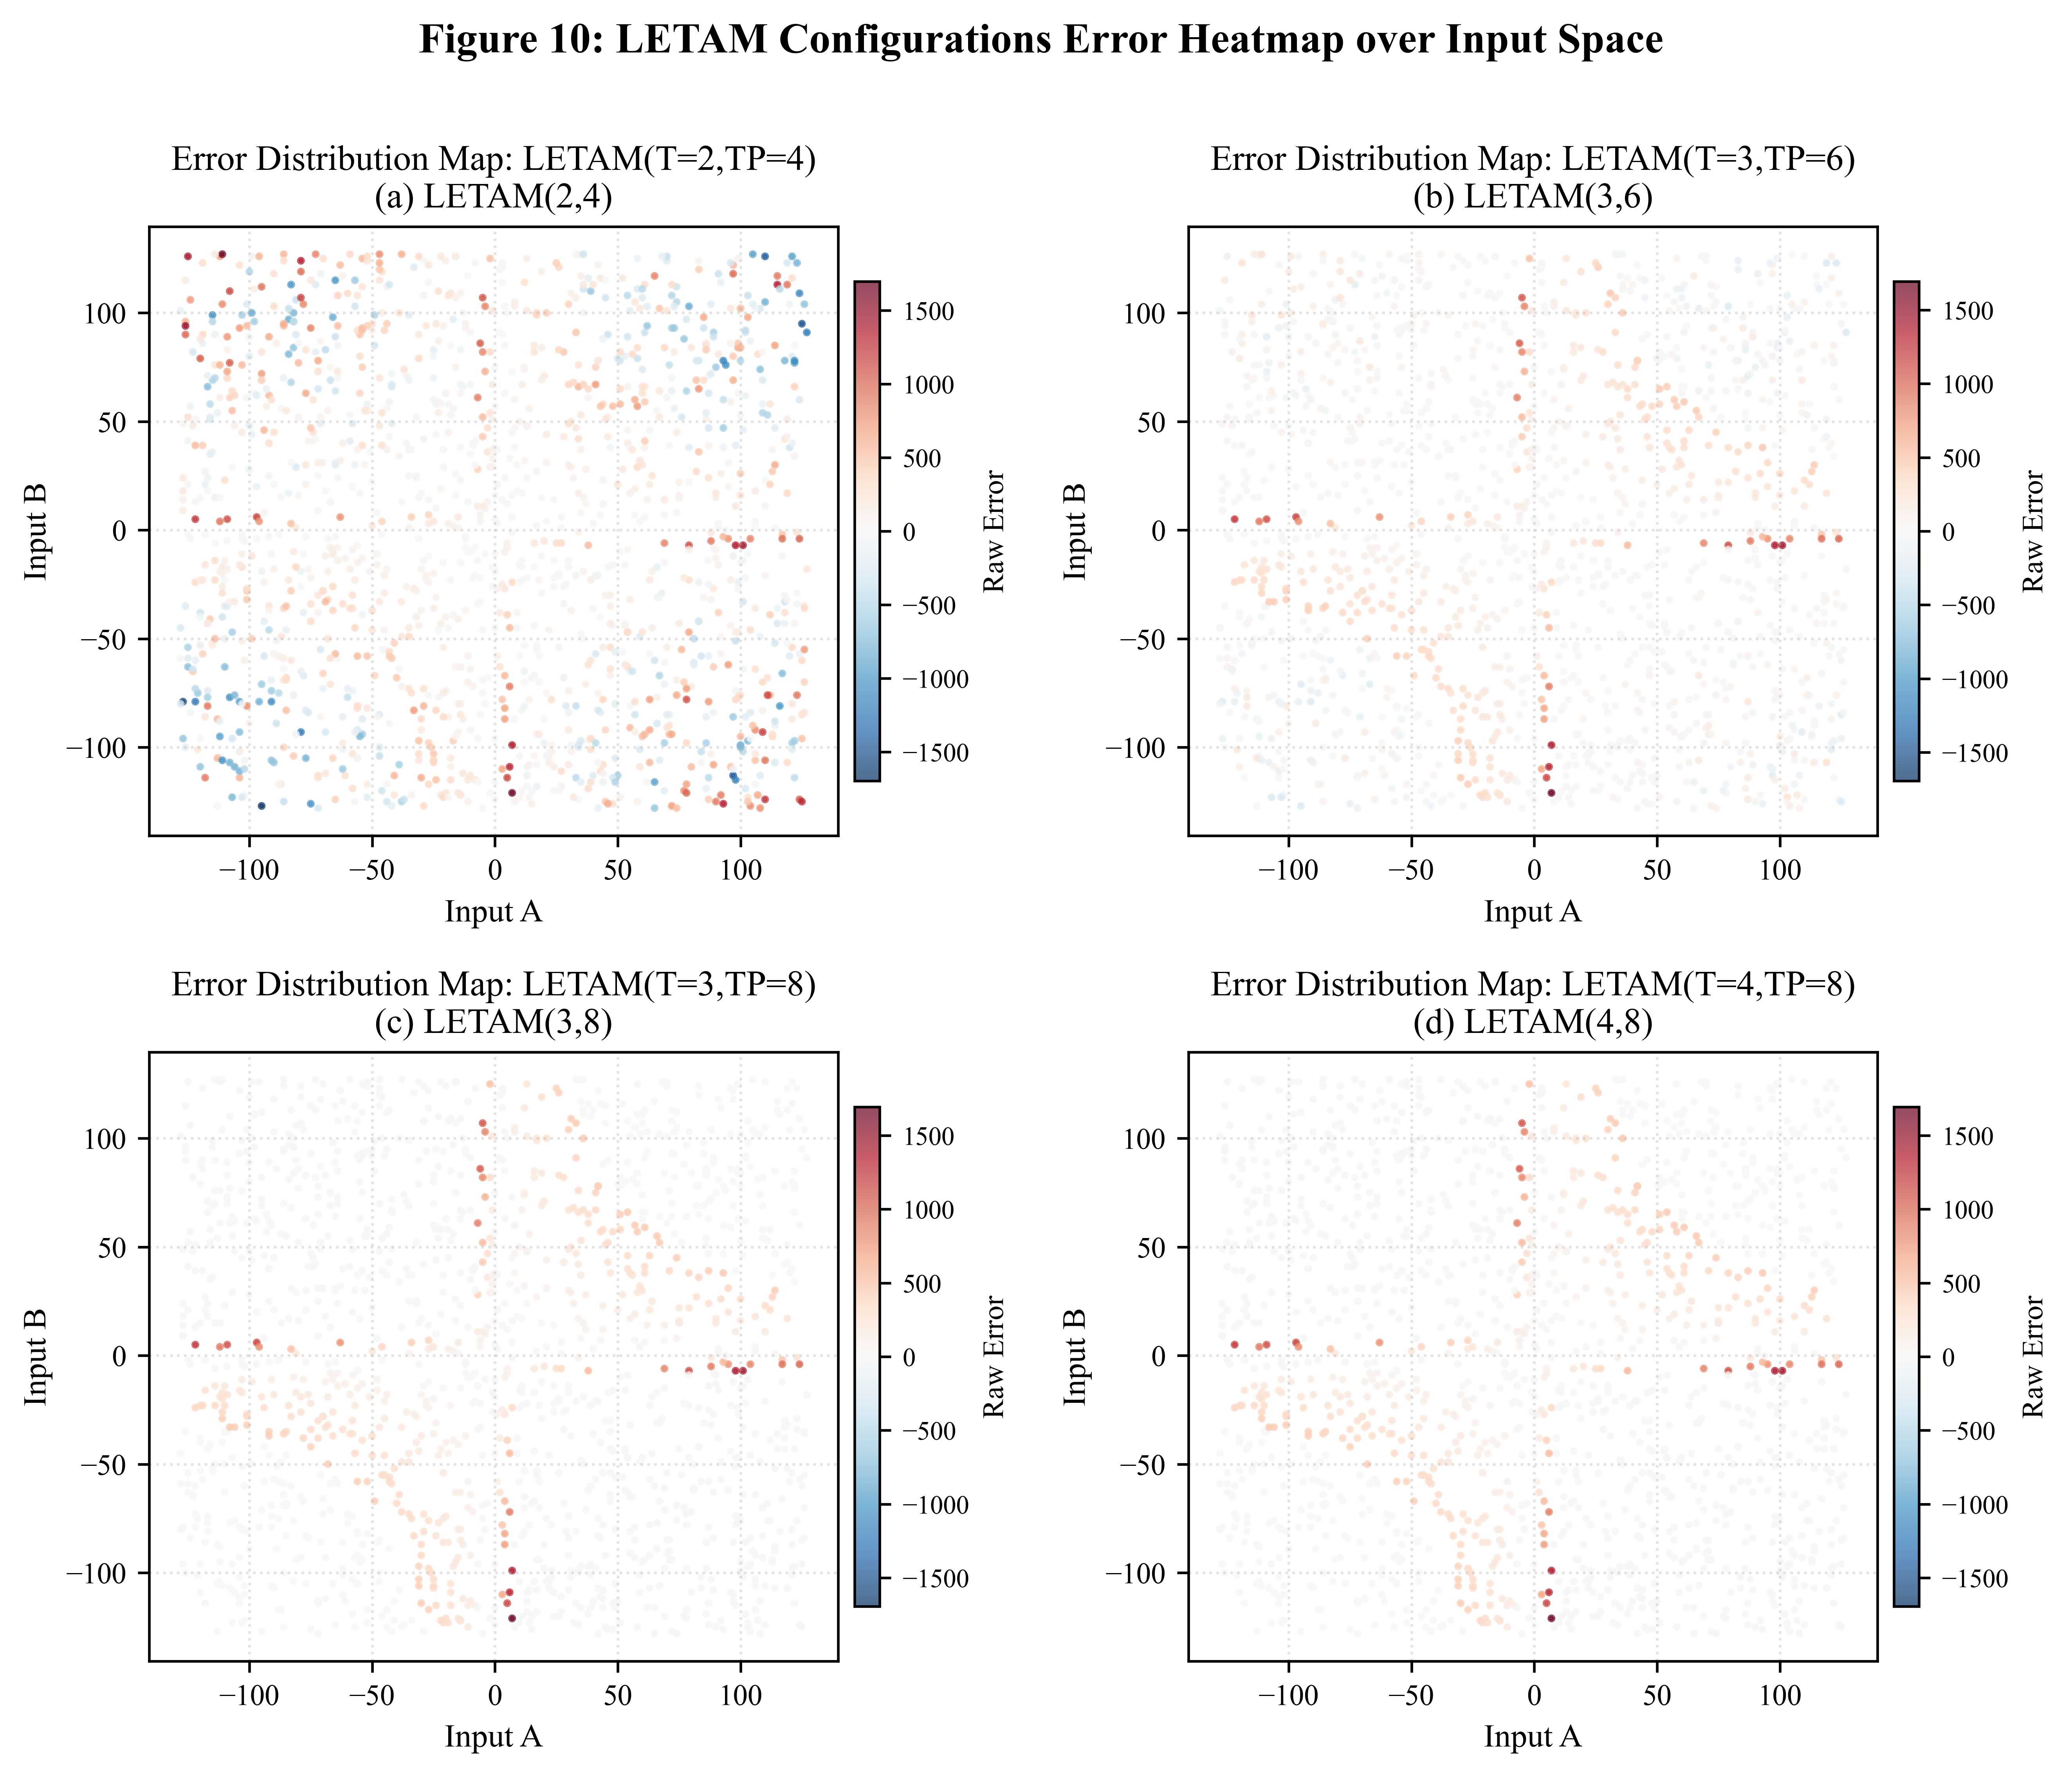
\includegraphics[width=0.95\textwidth]{LETAM_Fig10_heatmap}
\caption{LETAM全空间绝对误差热力图}
\label{fig:letam_heatmap}
\end{figure}

\clearpage
\subsection{算子级逻辑综合与 PPA 评估}
\label{subsec:ppa}

为全面量化近似乘法器架构对物理实现的具体影响，本研究基于 45\,nm Nangate 典型工艺库（1.0\,V，25\textcelsius），使用 
Synopsys Design Compiler 针对所设计的三类近似算子模型展开了逻辑综合与物理评估。综合工具阶段统
一关闭了扁平化（flatten）优化选项，以保留各计算子模块的原生层次结构。

\subsubsection{TOSAM 近似乘法器评估}

对于基于前导一检测与动态截断机制的 TOSAM 架构，设定若干档不同的低位尾数截取参数获取了对应的综合数据，
表~\ref{tab:tosam-ppa} 汇总了其与传统阵列乘法器的各项开销对比情况。

\begin{table}[htbp]
    \centering
    \caption{TOSAM 乘法器算子级物理综合结果对比 (45\,nm Nangate, 0.45\,GHz)}
    \label{tab:tosam-ppa}
    \small
    \setlength{\tabcolsep}{6pt}
    \begin{tabular}{lccc}
        \toprule
        乘法器配置 & 面积 ($\mu m^2$) & 功耗 ($\mu W$) & 时延 $t_{delay}$ \\
        \midrule
        精确基准 (\texttt{ExactSigned8bit})  & $314.14$            & $209.66$            & $1.30$  \\
        TOSAM(0,3)                         & $152.68$ ($-51.4\%$)  & $114.10$ ($-45.6\%$)  & $1.09$ ($-16.2\%$) \\
        TOSAM(1,4)                         & $207.75$ ($-33.9\%$) & $185.71$ ($-11.4\%$) & $1.41$ ($+8.5\%$) \\
        TOSAM(2,6)                         & $241.36$ ($-23.2\%$) & $241.23$ ($+15.1\%$) & $1.73$ ($+33.1\%$) \\
        TOSAM(3,7)                         & $291.54$ ($-7.2\%$) & $253.56$ ($+20.9\%$) & $2.05$ ($+57.7\%$) \\
        \bottomrule
    \end{tabular}
\end{table}

根据表~\ref{tab:tosam-ppa}提供的数据可知，TOSAM 在参数配置较小时（如 TOSAM(0,3)）
呈现出可观的硬件缩减能力。相较于传统 8 位精确乘法器，其面积近乎减半（$-51.4\%$），关键路径用时亦缩减了 16.2\%，
而且动态能耗更是显著降低了 45.6\%。这表明粗粒度截断机制确实大幅度简化了核心运算阵列规模。然而，随着保留段位宽与补偿复杂度的提升
（向 TOSAM(3,7) 演进），为重构精度所付出的线性调整与二次项非线性校正逻辑逐渐成为硬件瓶颈。高阶设计不仅面积红利被剧烈削减至
不到 10\%，且繁重的补偿多路累加操作导致了时延发生退行性恶化（$+57.7\%$），功耗更由原先的红利转为超过精确基准 20.9\% 的开销劣势。这反过来说明，TOSAM 的误
差平衡结构具有强烈的边际效用递减特性，更适合被约束部署在追求极致空间且允许大幅放宽精度的极限低能耗场景。

\subsubsection{ZBA-BM 近似乘法器评估}

不同于在原始操作数位宽上切除的动态截断方案，ZBA-BM 着眼于内部 Booth 编码简化与部分积树（PPSC）重构逻辑。表~\ref{tab:zbabm-ppa} 梳理了该架构下几种典型配置以及用作对照的无补偿基线的面积与动态功耗指标。

\begin{table}[htbp]
    \centering
    \caption{ZBA-BM 乘法器算子级物理综合结果对比 (45\,nm Nangate, 1\,GHz)}
    \label{tab:zbabm-ppa}
    \small
    \setlength{\tabcolsep}{6pt}
    \begin{tabular}{lccc}
        \toprule
        乘法器配置 & 面积 ($\mu m^2$) & 功耗 ($\mu W$) & 本征偏差 $\mu$ \\
        \midrule
        精确基准 (\texttt{ExactBooth8}, 4E0A)  & $291.54$            & $276.71$            & $0.000$  \\
        无补偿基线 (\texttt{KMap\_4Row\_ZG})   & $208.01$ ($-28.6\%$) & $234.29$ ($-15.3\%$) & $-0.125$ \\
        ZBA-BM 2E2A                          & $263.34$ ($-9.7\%$)  & $252.68$ ($-8.7\%$)  & $0.000$  \\
        ZBA-BM 1E3A                          & $241.53$ ($-17.2\%$) & $230.62$ ($-16.6\%$) & $0.000$  \\
        ZBA-BM 0E4A                          & $197.11$ ($-32.4\%$) & $202.67$ ($-26.8\%$) & $0.000$  \\
        \bottomrule
    \end{tabular}
\end{table}

综合数据表明，ZBA-BM 三档候选配置沿近似行数形成清晰的精度--PPA 轨迹：从 2E2A 到 1E3A 再到 0E4A，面积由
 $263.34$ 降至 $241.53$ 再到 $197.11~\mu m^2$（相对精确基线分别 $-9.7\%/-17.2\%/-32.4\%$），动态功耗由 $252.68$ 
 降至 $230.62$ 再到 $202.67~\mu W$（相对精确基线分别 $-8.7\%/-16.6\%/-26.8\%$）。无补偿基线 \texttt{KMap\_4Row\_ZG} 
 与 ZBA-BM 0E4A 在同等近似深度下的面积、功耗差距分别为 $5.3\%$ 与 $13.5\%$，说明 PPSC 的 Row-0 局部旁路并未破坏近似乘法
 器的主要 PPA 收益，却将本征偏差从 $-0.125$ 校正为 $0$。

\subsubsection{LETAM 近似乘法器评估}

不同于着眼尾段直接截去或编码局部旁路的传统设计，LETAM 架构引入了基于前导一检测与动态缩放的自适应量化机制。
表~\ref{tab:letam-ppa} 梳理了该架构的主推配置（即理论推荐基准 LETAM(3,6)）与用作对照的精确乘法器在面积、
功耗及关键路径时延方向的物理综合表现。

\begin{table}[htbp]
    \centering
    \caption{LETAM 乘法器算子级物理综合结果对比 (45\,nm Nangate, 0.93\,GHz)}
    \label{tab:letam-ppa}
    \small
    \setlength{\tabcolsep}{6pt}
    \begin{tabular}{lccc}
        \toprule
        乘法器配置 & 面积 ($\mu m^2$) & 功耗 ($\mu W$) & 时延 $t_{delay}$ (ns) \\
        \midrule
        精确基准 (\texttt{ExactSigned8bit}) & $314.14$            & $209.66$            & $1.30$ \\
        LETAM 基准配置 (\texttt{LETAM(3,6)})  & $317.07$ ($+0.9\%$) & $234.99$ ($+12.1\%$)& $1.08$ ($-16.9\%$) \\
        \bottomrule
    \end{tabular}
\end{table}

综合数据表明，由于 LETAM 内部集成了对数域映射、自适应移位对齐以及多路动态补偿重构等额外逻辑开销，
其整体电路排布发生了一度膨胀。与标准的 8 位精确基准（\texttt{ExactSigned8bit}）相比，其面积微增了
 $0.9\%$（至 $317.07~\mu m^2$），且复杂的控制网络与移位机制使得动态翻转能耗同步攀升了 $12.1\%$
 （至 $234.99~\mu W$）。然而，这种在空间与局部能耗上的妥协成功解耦了底层全精度阵列的冗长进位链连带动作。
 反映在核心物理时序指标上，LETAM 将最长计算路径的时延大幅压短至 $1.08\,\text{ns}$，斩获了高达 $16.9\%$ 
 的性能红利。这说明该方法有效突破了传统高阶近似补偿依赖深度串行逻辑引致时效恶化的固有瓶颈，在容许微量面
 积与功耗增长的前提下，换取了卓越的时序并行度收益与极强的主频提升底力。


\clearpage
\section{基于Gemmini的系统级架构集成}

\subsection{Chipyard SoC与Gemmini架构概述}

在敏捷硬件开发与深度学习加速器体系结构研究领域，Chipyard \cite{chipyard}
提供了一套统一的系统芯片（SoC）生成生态。该生态基于 Scala 与 Chisel 硬件构造语言构建，
全面集成了从 RISC-V 开源标量处理器（如 Rocket、BOOM）到各类片上总线、
缓存层次结构及特定领域加速器生成器的完整全栈式流程。
Gemmini \cite{gemmini-dac}则是寄宿于 Chipyard 平台下的一个开源的、高度参数化的脉动阵列（Systolic Array）
张量加速器生成器，其旨在探究 DNN 负载在包含访存机制与处理器协同情况下的系统级性能表现与实现上限。

架构层面上，Gemmini 作为专用矩阵乘法协处理器，通过 RoCC 接口与宿主 RISC-V 核心通信，并经 TileLink 总线访问共享主存
（如 L2 Cache 与外部 DRAM）。针对矩阵运算的高带宽需求，其内部采用脱耦的访问/执行（Decoupled Access/Execute）微架构。
硬件物理上被划分为并行的读写控制器与执行控制器，二者维护独立指令队列，由内置重排序缓冲区（ROB）协调数据依赖与写后读（RAW）等冲突。

\begin{figure}[htbp]
    \centering
    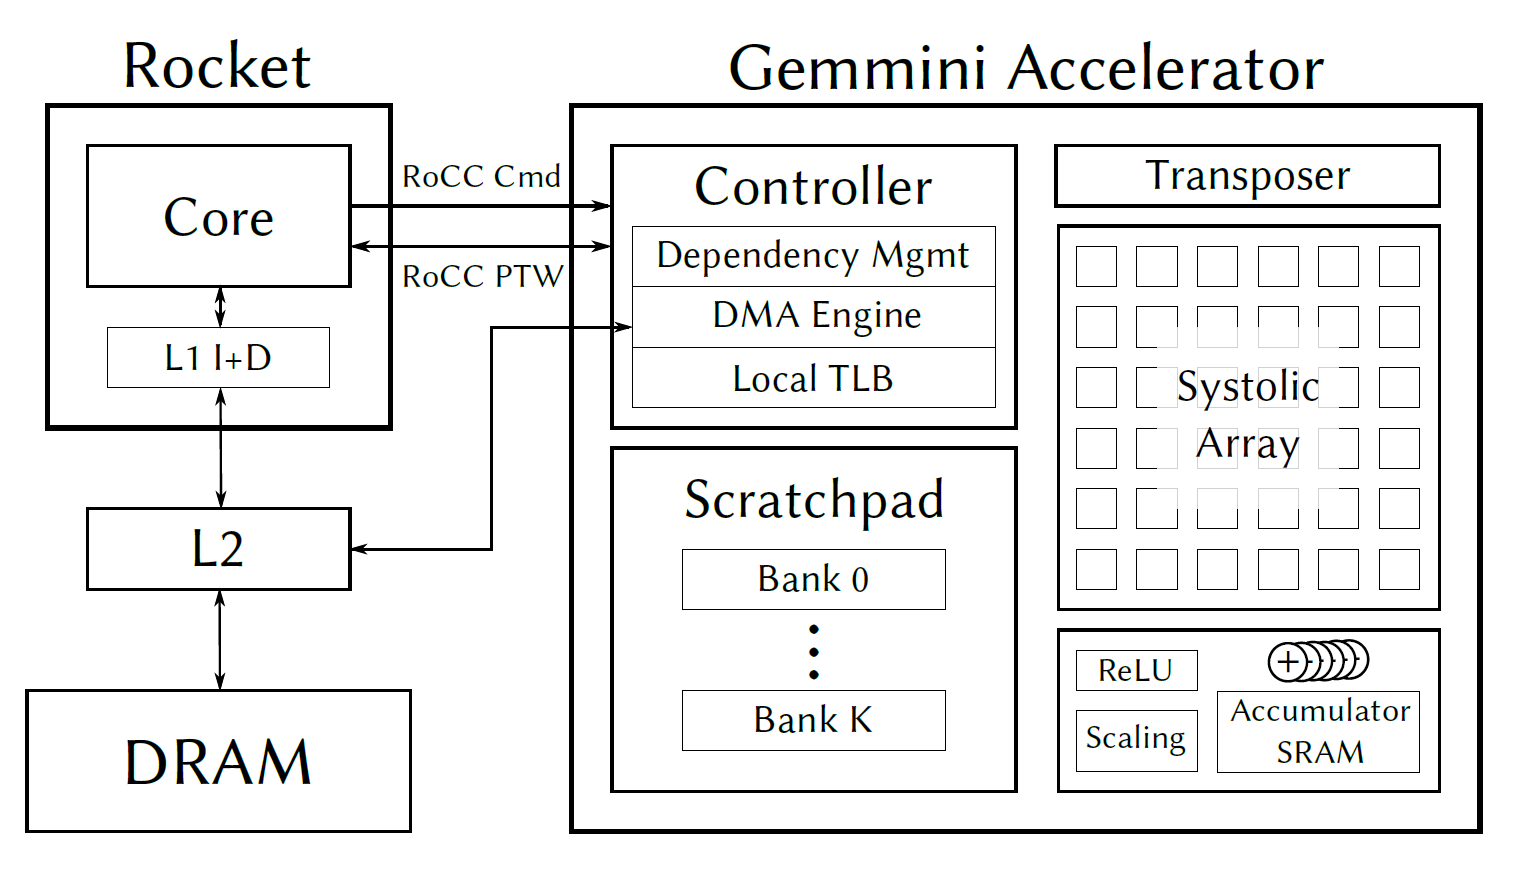
\includegraphics[width=0.8\textwidth]{gemmini-system.png}
    % \vspace{0.2em}
    \caption{Gemmini 协处理器系统级体系结构框架与存储分层示意图\cite{gemmini-dac}}
    \label{fig:gemmini-system}
\end{figure}

Gemmini 的核心为通用矩阵乘法（GEMM），
其性能与面积效率直接决定系统吞吐。在自然语言处理，尤其是 Transformer 
的前馈路径中，大量大尺寸矩阵变换对算力与带宽提出严格要求。
为此，Gemmini 在微结构上采用二维参数化的脉动阵列（systolic array），
由若干处理单元（Processing Element, PE）按网格组织形成块（Tile），
并以流水线寄存器连接相邻块。该阵列既支持权重驻留（weight‑stationary）
数据流，也可在不同位宽和拓扑下切换为输出驻留（output‑stationary）模式。
数据沿行列方向以连波（wavefront）方式推进，完成大规模并行的乘加（MAC）收敛，
从而在保持高并发的同时最大化算力与数据局部性。

\begin{figure}[htbp]
    \centering
    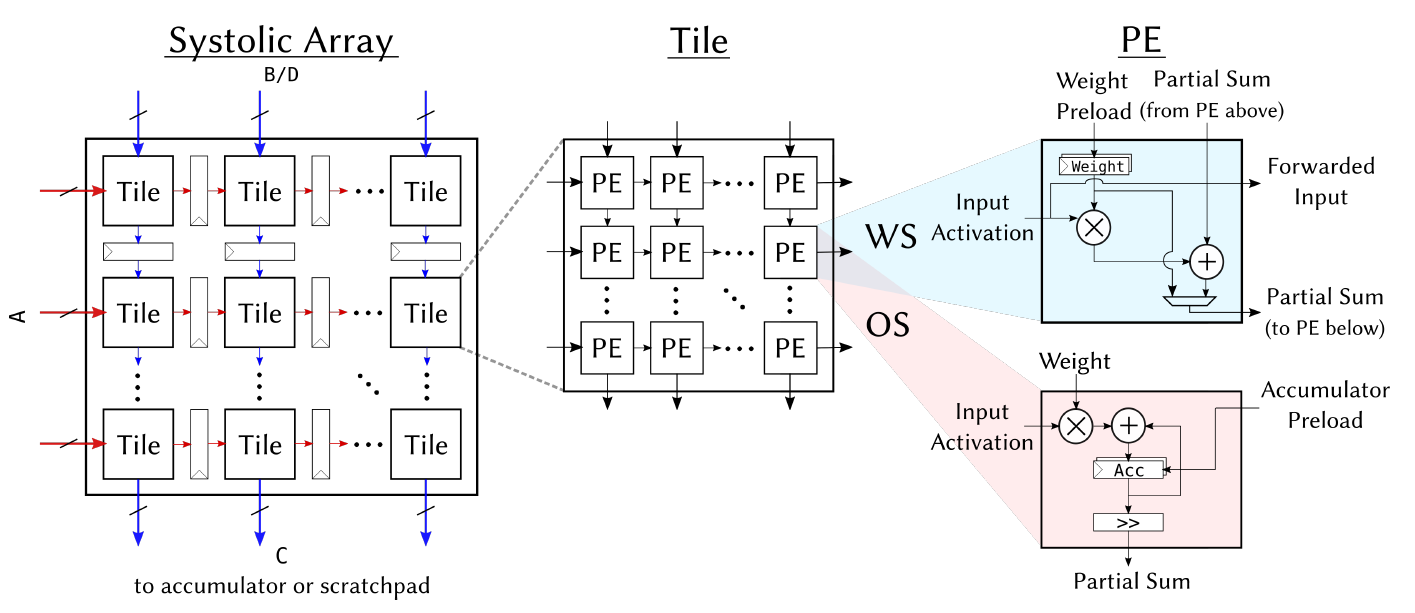
\includegraphics[width=0.8\textwidth]{gemmini-systolic-array.png}
    % \vspace{0.2em}
    \caption{Gemmini 两级并发的层级脉动阵列微结构与处理单元互连机制\cite{gemmini-dac}}
    \label{fig:gemmini-systolic}
\end{figure}

在本研究中，阵列内每个 PE 的精确乘法器构成
了面积与能耗的主要来源，其随网格规模二次增长而显著放大。
为建立从器件级近似到体系级效能的可验证路径，本文采
用工程化替换策略：在 PE 节点处以低功耗近似乘法器
替换原生精确乘法器。此方案在保持 Gemmini 时序与接口语义一致的前提下，
通过减小单体乘法器体积与关键路径长度，累积实现阵列级的功耗与面积优势，
同时便于在仿真与综合流程中量化误差传播与系统级 PPA 权衡。


\subsection{Scala生成器逻辑修改与底层适配}
为将近似乘法器嵌入 Gemmini 而不破坏既有指令语义、数据流控制和阵列互连，
本文采用“在最小可复用计算单元处局部替换”的集成策略，即将修改边界限定在
\texttt{PE} 内部的 \texttt{MacUnit}，而不改动 \texttt{Tile}、\texttt{Mesh} 以及上层
RoCC 接口。这一做法的核心考虑有二：其一，Gemmini 的权重驻留与输出驻留数据流均以 PE
中的乘加操作为基础，若直接替换 MAC 的乘法路径，则可在保持阵列时序组织不变的前提下
观察近似误差在系统中的真实传播；其二，局部封装便于后续在不同近似乘法器实现之间切换，
避免对生成器主体进行大范围侵入式修改。

具体实现上，首先在 \texttt{PE.scala} 中引入 \texttt{ApproxMulBlackBox}，
将外部 SystemVerilog 模块 \texttt{approx\_mul.sv} 封装为 Chisel 可识别的黑盒资源。
该黑盒接口固定为两个有符号 $8$ bit 输入和一个有符号 $16$ bit 输出，
与 Gemmini 缺省整型阵列的 \texttt{SInt(8.W)} 乘法通路保持一致。
在此基础上，本文进一步为 \texttt{MacUnit} 增加参数 \texttt{useApproxMul}，
当该参数置位时，原先的精确表达式 \texttt{io.in\_c.mac(io.in\_a, io.in\_b)}
被替换为“近似乘积 + 原累加项”的组合实现；否则仍保留原始精确 MAC 路径。
这样一来，近似乘法器仅改变乘法结果的生成方式，而输入输出位宽、累加器写回路径、
控制寄存器切换以及 OS/WS 两种数据流下的状态推进逻辑均不需要额外改写。
从工程角度看，这种参数化接入方式确保了近似单元对 Gemmini 生成器的影响被限制在
局部算术单元内部，具有较好的可维护性与可复现性。

值得说明的是，近似乘法器的接入并非简单地以 Verilog 文件替换精确乘法器即可完成，
而需要同时处理类型适配与资源绑定问题。Gemmini 原始 \texttt{MacUnit} 为泛型设计，
而本文所接入的近似乘法器仅面向有符号 $8$ bit 整型输入，因此在 Scala 侧通过
\texttt{require} 语句显式限定了输入类型与位宽；与此同时，利用
\texttt{addResource("/vsrc/approx\_mul.sv")} 将底层 RTL 纳入生成系统，
保证 Verilator 编译与后续综合流程均可自动解析该外部模块。由此形成的层级依赖关系可概括为
\texttt{MeshWithDelays $\rightarrow$ Tile $\rightarrow$ PE\_256 $\rightarrow$ MacUnit $\rightarrow$ approx\_mul}，
其中特定近似算法仅作用于最末端乘法节点，阵列级数据搬移与调度机制保持不变。

\begin{lstlisting}[caption={Gemmini 中近似乘法路径的关键生成器改动},label={lst:approx-gemmini-scala},language=Java,basicstyle=\ttfamily\small]
class ApproxMulBlackBox extends BlackBox with HasBlackBoxResource {
  override def desiredName = "approx_mul"
  val io = IO(new Bundle {
    val a = Input(SInt(8.W))
    val b = Input(SInt(8.W))
    val result = Output(SInt(16.W))
  })
  addResource("/vsrc/approx_mul.sv")
}

if (useApproxMul) {
  val approx_mul = Module(new ApproxMulBlackBox)
  approx_mul.io.a := io.in_a.asTypeOf(SInt(8.W))
  approx_mul.io.b := io.in_b.asTypeOf(SInt(8.W))
  io.out_d := (approx_mul.io.result +&
    io.in_c.asTypeOf(SInt(io.in_c.getWidth.W))).asTypeOf(io.out_d)
} else {
  io.out_d := io.in_c.mac(io.in_a, io.in_b)
}
\end{lstlisting}

上述改动的一个直接收益在于：当 \texttt{approx\_mul.sv} 的端口定义保持稳定时，
后续替换不同近似乘法器版本无需重新设计 Gemmini 的 Chisel 结构，
仅需重新触发相应后端编译流程即可完成更新。这使本文能够将研究重点集中于“近似乘法器对系统行为的影响”
而非反复处理大规模生成器重构问题，为后续综合、仿真和误差分析提供了清晰的工程基础。

\subsection{仿真测试}
\label{subsec:simulation}
在完成生成器适配之后，本文进一步建立了覆盖“编译、综合、仿真”三个环节的复现链路。
前端采用 Chipyard/Gemmini 的 Scala/Chisel 生成器完成 SoC 级硬件展开，
并通过 \texttt{firtool} 导出可综合的 SystemVerilog；仿真端使用 Verilator 构建
\texttt{simulator-chipyard.harness-ApproxGemminiRocketConfig}，
软件端则编译裸机测试程序 \texttt{approx\_matmul\_test.c}；综合端将提取出的
\texttt{approx\_mul}、\texttt{MacUnit}、\texttt{PE}、\texttt{Tile}、
\texttt{Mesh} 与 \texttt{MeshWithDelays} 等层级送入 Design Compiler，
生成面积、功耗与时序报告。整个流程既覆盖了从生成器到 RTL 的静态实现路径，
也覆盖了从 CPU 发起调用到阵列返回结果的动态执行路径。

\begin{figure}[htbp]
    \centering
    \begin{tikzpicture}[
        node distance=8mm and 6mm,
        >=Latex,
        font=\small,
        box/.style={rectangle, rounded corners=2pt, draw=black, align=center, text width=2.75cm, minimum height=0.95cm, fill=gray!8},
        line/.style={-Latex, thick}
    ]
        \node[box] (rtl) {近似乘法器 RTL\\\texttt{approx\_mul.sv}};
        \node[box, right=of rtl] (scala) {Gemmini 生成器适配\\\texttt{PE.scala}\\\texttt{MacUnit}};
        \node[box, right=of scala] (elab) {Chipyard 展开与 RTL 导出\\Scala/Chisel + \texttt{firtool}};
        \node[box, below=of elab] (sim) {Verilator SoC 仿真器\\\texttt{ApproxGemmini}\\\texttt{RocketConfig}};
        \node[box, left=of sim] (cprog) {裸机矩阵乘法程序\\\texttt{approx\_matmul}\\\texttt{\_test.c}};
        \node[box, right=of sim] (check) {CPU 精确基准对比\\误差统计与结果分析};
        \node[box, right=of elab] (dc) {Design Compiler 综合\\面积/功耗/时序报告};

        \draw[line] (rtl) -- (scala);
        \draw[line] (scala) -- (elab);
        \draw[line] (elab) -- (sim);
        \draw[line] (cprog) -- (sim);
        \draw[line] (sim) -- (check);
        \draw[line] (elab) -- (dc);
    \end{tikzpicture}
    \caption{近似乘法器集成 Gemmini 的复现与验证流程}
    \label{fig:approx-gemmini-flow}
\end{figure}

\subsubsection{4$\times$4 裸机矩阵乘法链路验证}

软件验证采用裸机方式而非 Linux 用户态程序，其目的在于尽量缩短软件栈路径，
使观测结果更直接地反映硬件本体行为。测试程序首先在 CPU 侧完成精确矩阵乘法，
得到 $32$ bit 累加精度下的基准结果；随后通过 \texttt{gemmini\_mvin} 将输入矩阵搬入
片上存储，通过 \texttt{gemmini\_preload\_zeros} 与
\texttt{gemmini\_compute\_preloaded} 触发 Gemmini 阵列计算，
最后使用 \texttt{gemmini\_mvout} 读回累加器结果，并逐元素与 CPU 基准比较。
这一流程确保了“软件可见结果”与“阵列内部近似乘法行为”之间建立起明确映射。

\begin{lstlisting}[caption={$4\times4$ 裸机矩阵乘法测试的核心调用序列},label={lst:approx-gemmini-c},language=C,basicstyle=\ttfamily\small]
cpu_matmul(A, B, C_ref);
gemmini_mvin(A_full, A_sp_addr);
gemmini_mvin(B_full, B_sp_addr);
gemmini_preload_zeros(C_acc_addr);
gemmini_compute_preloaded(A_sp_addr, B_sp_addr);
gemmini_mvout(C_acc, C_acc_read_addr);
\end{lstlisting}

本文最终跑通了一个 $4\times4$ 矩阵乘法程序（以TOSAM(3,7)近似乘法器为实现）。设输入矩阵为
\[
\mathbf{A}=\begin{bmatrix}
31 & -28 & -25 & -22 \\
24 & -21 & -18 & -15 \\
17 & -14 & -11 & -8 \\
10 & -7 & -4 & -1
\end{bmatrix},\qquad
\mathbf{B}=\begin{bmatrix}
30 & 19 & 8 & 3 \\
25 & 14 & 3 & 8 \\
20 & 9 & 2 & 13 \\
15 & 4 & 7 & 18
\end{bmatrix}.
\]
CPU 参考结果与近似Gemmini加速器的仿真结果分别为
\[
\mathbf{C}_{\mathrm{CPU}}=\mathbf{A}\mathbf{B}=\begin{bmatrix}
2460 & 1294 & 128 & -1038 \\
1830 & 972 & 114 & -744 \\
1200 & 650 & 100 & -450 \\
570 & 328 & 86 & -156
\end{bmatrix},
\]
\[
\mathbf{C}_{\mathrm{Gemmini}}=\begin{bmatrix}
2503 & 1311 & 132 & -1058 \\
1867 & 980 & 115 & -762 \\
1213 & 658 & 100 & -458 \\
582 & 332 & 87 & -158
\end{bmatrix}.
\]
据此，元素级误差矩阵为
\[
\mathbf{E}=\mathbf{C}_{\mathrm{Gemmini}}-\mathbf{C}_{\mathrm{CPU}}=\begin{bmatrix}
43 & 17 & 4 & -20 \\
37 & 8 & 1 & -18 \\
13 & 8 & 0 & -8 \\
12 & 4 & 1 & -2
\end{bmatrix}.
\]

从矩阵形式结果可以看出，Gemmini 输出与 CPU 基准在符号上保持一致，偏差主要体现为幅值上的轻微漂移。
在 $16$ 个矩阵元素中，有 $15$ 个出现数值偏差，仅 $1$ 个元素与参考值完全一致。
从统计指标看，最大绝对误差为 $43$，平均绝对误差为 $12.25$，均方根误差为 $17.27$，
说明当前实现已完成从矩阵乘法输入、阵列计算到结果回传的完整闭环，但仍存在可进一步优化的数值误差。


在工具链层面，本文已经完成从前端生成、后端编译到独立综合的闭环验证：一方面，Verilator 仿真证明了所设计近似单元能够嵌入 Chipyard-Gemmini SoC 并通过裸机程序触发矩阵乘法计算；另一方面，基于 Design Compiler 的综合流程也已经跑通，能够对导出的独立 RTL 生成面积、功耗与时序报告，为算子级 PPA 分析提供数据基础。$4 \times 4$ 裸机程序的成功运行表明本文提出的近似算术单元并非停留于孤立电路级验证，而是已经能够作为 Gemmini 体系结构中的真实计算资源参与仿真执行。

\subsubsection{矩阵累加误差的 Frobenius 尺度律}
为统一描述矩阵乘法中的误差累加，本文使用单次乘法误差的均值 $\mu$ 与标准差 $\sigma$
刻画近似乘法器的统计特征。设 $m$ 为单个输出元素对应的内积长度，
$L_{\mathrm{eff}}$ 为同一前向路径中可视作连续累加的有效次数。
在均匀输入与独立误差假设下，输出元素的未缩放累加误差可用下式估计\cite{liu2025frobenius}：
\begin{equation}
\label{eq:frob-rms-out}
\widehat{\mathrm{RMS}}_{\!E}(m,L_{\mathrm{eff}}) =
\sqrt{L_{\mathrm{eff}}\,m\,\sigma^2 + \bigl(L_{\mathrm{eff}}\,m\,\mu\bigr)^2}.
\end{equation}
式~\eqref{eq:frob-rms-out} 中，方差项随 $L_{\mathrm{eff}}\,m$ 线性增长，开方后对应
$\mathcal{O}(\sqrt{L_{\mathrm{eff}}\,m})$；均值项随 $L_{\mathrm{eff}}\,m$ 累加，开方后对应
$\mathcal{O}(L_{\mathrm{eff}}\,m)$。该公式仅依赖算子级全遍历即可获取的 $\mu$ 与 $\sigma$
两个统计量，即可在无需实际运行系统级仿真的前提下，快速预测不同矩阵乘规模下的误差增长趋势，
为后续系统级实验与应用级评估提供先验参照。

\subsubsection{ResNet-50 \texttt{conv1} 真实卷积层验证}
\label{subsec:zbabm-tosam-resnet}

本节使用 ResNet-50 第一层卷积 \texttt{conv1} 作为系统级输出样例，
检查近似乘法器进入 Gemmini 数据通路后的输出误差。实验分别运行精确基线 exact、
ZBA-BM 2E2A 与 TOSAM$(3,7)$ 三条周期级链路。三条链路共享同一 ResNet-50 量化权重，
输入图像为 CIFAR-10 测试集第 0 张经 int8 量化后的结果，数据流配置保持一致，
仅替换 PE 内部的乘法器实现。

\texttt{conv1} 卷积输出经后续 $3\times3$ max-pool 下采样后，
张量形状为 $1 \times 56 \times 56 \times 64$，共 $200\,704$ 个 int8 元素，
单点累加深度为 $K=147$。表~\ref{tab:zbabm-tosam-resnet} 中的数值为最终 8 bit 输出误差，
包括 ME、MAE、RMSE、Frobenius 范数、余弦相似度以及符号/零值错误计数。
这些指标已经包含卷积输出缩放、截断和饱和等后处理，与式~\eqref{eq:frob-rms-out}
中的原始累加器误差不处于同一量纲。

\begin{table}[htbp]
    \centering
    \caption{ResNet-50 \texttt{conv1} 输出的系统级误差对比}
    \label{tab:zbabm-tosam-resnet}
    \small
    \setlength{\tabcolsep}{5pt}
    \begin{tabular}{lccc}
        \toprule
        指标 & exact & ZBA-BM 2E2A & TOSAM$(3,7)$ \\
        \midrule
        ME           & $0.0000$  & $+0.0641$  & $+0.0779$ \\
        MAE          & $0.0000$  & $2.7625$   & $0.1663$ \\
        RMSE         & $0.0000$  & $4.2046$   & $0.4105$ \\
        MaxAbs       & $0$       & $34$       & $2$ \\
        Frobenius    & $0.0000$  & $1883.6767$ & $183.9185$ \\
        Cosine       & $1.0000$  & $0.9676$   & $0.9997$ \\
        Sign Errors  & $0$       & $6312$     & $166$ \\
        \bottomrule
    \end{tabular}
\end{table}

表中结果显示，TOSAM$(3,7)$ 在所有指标上均优于 ZBA-BM 2E2A。
TOSAM$(3,7)$ 的 RMSE 为 $0.4105$，ZBA-BM 2E2A 为 $4.2046$，二者相差约一个数量级；
Frobenius 范数呈现相同的差距比例。
余弦相似度方面，TOSAM$(3,7)$ 达到 $0.9997$，而 ZBA-BM 2E2A 为 $0.9676$，
后者的符号与零值错误计数也高出近 $38$ 倍。

该结果与算子级全遍历统计一致。在 $K{=}147$ 的短链累加深度下，
输出误差主要受单乘误差方差 $\sigma^2$ 支配，
方差较小的 TOSAM$(3,7)$ 直接对应更低的系统级输出失真。
均值偏差 $\mu$ 的累积效应在此累加深度下尚未充分显现，
其影响将在第五章更大规模的矩阵乘场景中进一步讨论。

\subsection{面向稀疏大矩阵的系统级扩展设计}
\label{subsec:system-extension}

前述系统级仿真表明，近似乘法器可以在不改变 Gemmini 阵列外部接口的条件下进入真实数据通路。
基于这一集成边界，面向稀疏大矩阵推理的进一步设计可以继续限定在 PE 内部，
而不改动 \texttt{Tile}、\texttt{Mesh}、RoCC 指令语义以及累加器写回协议。
具体而言，\texttt{approx\_level} 或 \texttt{useApproxMul} 信号只负责选择精确乘法路径与近似乘法路径，
使不同精度路径的选择成为运行时配置问题，而不是重新生成整套 Gemmini 结构。

\begin{figure}[htbp]
    \centering
    \includegraphics[width=0.95\textwidth]{PicDoc/PicDoc_2026-04-28+20_12_17.png}
    \caption{面向稀疏大矩阵推理的系统级扩展设计}
    \label{fig:sparse-system-extension}
\end{figure}

图~\ref{fig:sparse-system-extension} 给出了该扩展设计的接口位置。阵列拓扑和片上数据流保持不变，
精确/近似乘法选择、输入零值识别与局部操作数隔离集中在 PE 乘法入口附近完成。
当输入操作数中存在零值时，PE 可在乘法器入口处进行操作数隔离或时钟使能屏蔽；
当输入不为零时，数据仍沿精确、近似双路径进入同一累加结构。

\subsubsection{输入零值稀疏性利用}

深度神经网络中间层的激活张量通常包含大量零值，尤其是经 ReLU 激活后，
零值比例可达 50\% 以上\cite{mrazek2019alwann}。对于脉动阵列而言，
零操作数参与的乘加运算不产生有效信息，但仍消耗乘法器的开关功耗。
在近似乘法器场景下，零操作数的乘法不仅浪费功耗，
还可能因近似误差引入不必要的非零残差。
因此，在 PE 乘法入口处增加零值检测逻辑具有双重收益：
一方面通过时钟门控或操作数隔离降低动态功耗，
另一方面避免近似乘法器对零输入产生虚假误差。
该检测逻辑仅需对 8 bit 操作数执行全零判断，硬件开销为一个 8 输入 NOR 门，
相对 PE 整体面积可忽略不计。

\subsubsection{动态层级精度分配}

DNN 各层对近似误差的容忍度并不均匀。
ALWANN\cite{mrazek2019alwann} 等研究表明，浅层特征提取对精度要求较高，
而深层分类层的冗余度较大，可以承受更高的近似深度。
ZBA-BM 的多档配置 2E2A、1E3A 与 0E4A 天然构成一个精度--PPA 调节池：
三档配置共享相同的零均值性质，但面积分别为精确基线的 $90.3\%$、$82.8\%$ 与 $67.6\%$，
对应不同层级的误差容忍需求。

在 Gemmini 的 RoCC 指令接口中，\texttt{approx\_level} 字段已预留 2 bit 配置空间，
足以编码精确、2E2A、1E3A、0E4A 四种模式。
编译器或运行时调度器可根据各层的累加深度 $K$ 与误差敏感度，
为每一层的 GEMM 调用指定相应的近似档位，
从而在不修改网络结构和权重的前提下，
实现全网络范围内面积与精度的帕累托权衡。

上述零值门控与动态精度分配均已在系统级结构中完成接口预留，
但相关的门控功耗收益、层级精度搜索策略以及端到端精度影响，
在未来仍需在统一的 RTL--PPA--应用评估流程中进一步验证。

\clearpage
\section{面向大语言模型的应用级精度评估}
\label{sec:experiments}

第四章的系统级仿真验证了近似乘法器在 $K{=}147$ 的卷积层中的误差表现。
然而，现代大语言模型的矩阵乘规模远超卷积场景，
单次线性投影的内积长度可达数千，且前向路径中包含数十层连续的矩阵变换。
在此尺度下，近似误差的累积行为是否仍可接受，
需要从理论预测和端到端应用指标两方面加以评估。

大语言模型推理中的主要计算对象是由 Transformer 注意力投影与前馈网络构成的大规模矩阵乘。
$Q/K/V/O$ 投影、FFN 的升维与降维投影以及门控投影均可表示为激活矩阵与权重矩阵的乘加，
近似乘法器若用于量化推理，实际替换的是每个 MAC 中的 $8$ bit 激活--权重乘法，
再由累加器形成输出特征。标准 Transformer 的 self-attention 输出可写为
\[
\mathrm{Attention}(Q,K,V)=\mathrm{softmax}(QK^{T}/\sqrt{d_k})V,
\]
其中包含对 Value 向量的加权求和\cite{vaswani2017attention}。
在自回归语言模型中，新 token 的表示依赖此前上下文中所有 token 的表示。
以 GPT-3\cite{brown2020language} 为代表的大规模语言模型采用 96 层 Transformer、
隐藏维度 12288 的深层堆叠结构，长上下文推理涉及跨数千 token 的连续聚合，
使得前向路径中等效累加深度 $L_{\mathrm{eff}}\,m$ 可达极高量级。
对于近似乘法器而言，这意味着即使单次乘法误差的均值偏差 $\mu$ 极小，
经过如此深度的累积仍可能产生不可忽略的输出失真，
这正是本文关注零均值设计并在大规模矩阵乘场景中验证其优势的核心动机。
基于这一结构，本章先使用式~\eqref{eq:frob-rms-out} 估计未缩放累加器误差，
再通过 TinyLlama-1.1B 的逐 token 困惑度 PPL 报告应用级结果。
前者用于在公式假设下比较不同规模点上的误差增长趋势，
后者则在给定模型和数据集上衡量近似乘法对语言建模质量的实际影响。

\subsection{LLM 矩阵乘中的 Frobenius 失真预测}
\label{subsec:llm-frobenius}

LLM 推理中的线性投影、FFN 投影与注意力聚合通常具有比 \texttt{conv1} 更长的内积长度和更多连续计算步骤。
为观察近似误差在不同矩阵乘规模下的增长趋势，本文沿用式~\eqref{eq:frob-rms-out}
进行未缩放累加器误差估计。表~\ref{tab:frob-llm} 使用的输入来自 8 位全遍历算子统计：
ZBA-BM 2E2A 取 $\mu=0,\sigma=147.80$，TOSAM$(3,7)$ 取 $\mu=-0.009521,\sigma=72.90$。
计算时将各场景的 $mL_{\mathrm{eff}}$ 代入公式，得到预测每元素输出 RMS 失真
$\widehat{\mathrm{RMS}}_{\!E}$。

需要指出，表~\ref{tab:frob-llm} 中的数值为未经输出缩放和饱和处理的原始累加器误差尺度，
仅用于比较同一公式假设下不同规模点之间的相对增长趋势。

具体场景中，ResNet-50 \texttt{conv1} 取实测层 $m=3\times7\times7=147,L_{\mathrm{eff}}=1$；
TinyLlama-1.1B 取隐藏维度 $m=2048$、FFN 中间维度 $m=5632$ 与层数 $L_{\mathrm{eff}}=22$；
更大模型规模点采用各自的 FFN 内积长度与主干线性投影累计次数。
长上下文 Attention 聚合参照用于表示跨 token 连续求和下的高累加深度设置，
不对应本文已经完成的周期级系统仿真。

\begin{table}[htbp]
    \centering
    \caption{不同矩阵乘规模下的预测每元素输出 RMS 失真对比}
    \label{tab:frob-llm}
    \small
    \setlength{\tabcolsep}{5pt}
    \resizebox{\textwidth}{!}{%
    \begin{tabular}{lccc}
        \toprule
        场景 & $mL_{\mathrm{eff}}$ & TOSAM$(3,7)$ $\widehat{\mathrm{RMS}}_{\!E}$ & ZBA-BM 2E2A $\widehat{\mathrm{RMS}}_{\!E}$ \\
        \midrule
        ResNet-50 \texttt{conv1} ($m{=}147,L{=}1$)        & $1.5\!\times\!10^{2}$ & $8.84\!\times\!10^{2}$ & $1.79\!\times\!10^{3}$ \\
        TinyLlama hidden 投影 ($m{=}2048,L{=}22$)         & $4.5\!\times\!10^{4}$ & $1.55\!\times\!10^{4}$ & $3.14\!\times\!10^{4}$ \\
        TinyLlama FFN 投影 ($m{=}5632,L{=}22$)            & $1.2\!\times\!10^{5}$ & $2.57\!\times\!10^{4}$ & $5.20\!\times\!10^{4}$ \\
        LLaMA-65B 级 FFN ($m{=}32768,L{=}320$)            & $1.0\!\times\!10^{7}$ & $2.56\!\times\!10^{5}$ & $4.79\!\times\!10^{5}$ \\
        GPT-3 175B 级 FFN ($m{=}49152,L{=}384$)           & $1.9\!\times\!10^{7}$ & $3.64\!\times\!10^{5}$ & $6.42\!\times\!10^{5}$ \\
        长上下文 Attention 聚合参照                          & $1.0\!\times\!10^{9}$ & $9.80\!\times\!10^{6}$ & $4.67\!\times\!10^{6}$ \\
        \bottomrule
    \end{tabular}
    }
\end{table}

表中呈现出两段不同的趋势。
在 ResNet-50 \texttt{conv1} 到 GPT-3 175B 级 FFN 的五个规模点上，
误差增长主要由方差项 $L_{\mathrm{eff}}\,m\,\sigma^2$ 主导，
TOSAM$(3,7)$ 凭借更小的 $\sigma$ 始终保持较低的预测失真。
然而在长上下文 Attention 聚合参照点处，$L_{\mathrm{eff}}\,m$ 达到 $10^9$ 量级，
均值项 $(L_{\mathrm{eff}}\,m\,\mu)^2$ 的二次增长开始追上方差项的线性增长。
TOSAM$(3,7)$ 因 $\mu{=}{-}0.0095$ 而在此处被放大至 $9.80\times10^{6}$，
反超 ZBA-BM 2E2A 的 $4.67\times10^{6}$。
这一交叉正是式~\eqref{eq:frob-rms-out} 中 $\mathcal{O}(L_{\mathrm{eff}}\,m)$
均值项与 $\mathcal{O}(\sqrt{L_{\mathrm{eff}}\,m})$ 方差项增长阶数差异的直接体现。
换言之，在中小规模矩阵乘中，方差较低的 TOSAM$(3,7)$ 表现更优；
但当累加深度增长至 LLM 长上下文推理所对应的量级时，
ZBA-BM 2E2A 凭借 $\mu{\equiv}0$ 的零均值性质，
其预测失真反而低于存在微小负偏差的 TOSAM$(3,7)$。
这一结果表明，零均值设计在面向大规模矩阵乘的近似乘法器中具有不可替代的结构性优势。

\subsection{TinyLlama 困惑度评估}
\label{subsubsec:llm_tinyllama}
\label{subsec:zbabm-tosam-llm}

Frobenius 尺度估计只描述矩阵输出扰动能量，不能替代语言模型质量评估。
为补充应用层观测，本文在 TinyLlama-1.1B-Chat-v1.0 上完成 PPL 评测。
数据集采用 wikitext-2 raw test split，token 总数为 $341\,469$，推理时使用 stride 滑窗。
模型配置为 hidden size $2048$、$22$ 层、FFN intermediate size $5632$。
所有近似配置在同一前向通路中以 $256\times256$ LUT 替换 \texttt{nn.Linear}
内部的 $8$ bit $\times$ $8$ bit 整型乘法，输出层保持精确以避免词表投影引入额外变量。
表~\ref{tab:zbabm-tosam-ppl} 汇总逐 token PPL 结果，其中 PPL 越低表示语言建模质量越接近 exact 基线。

\begin{table}[htbp]
    \centering
    \caption{TinyLlama-1.1B 在 wikitext-2 (test) 上的逐 token PPL 实测对比}
    \label{tab:zbabm-tosam-ppl}
    \small
    \setlength{\tabcolsep}{5pt}
    \begin{tabular}{lcc}
        \toprule
        配置 & PPL & 相对 exact 退化 \\
        \midrule
        exact（精确乘法基线）        & $7.0952$ & --- \\
        TOSAM$(3,7)$               & $8.6207$ & $+21.50\%$ \\
        ZBA-BM 2E2A                & $8.7807$ & $+23.76\%$ \\
        ZBA-BM 1E3A                & $12.2867$ & $+73.17\%$ \\
        \texttt{KMap\_4Row\_ZG}    & $102.94$ & $+1350.86\%$ \\
        \bottomrule
    \end{tabular}
\end{table}

TOSAM$(3,7)$ 与 ZBA-BM 2E2A 的 PPL 分别为 $8.6207$ 与 $8.7807$，
相对 exact 基线的退化差距仅为 $2.26$ 个百分点，
表明二者在该评测设置下的应用级精度处于同一水平。

ZBA-BM 1E3A 的 PPL 退化至 $+73.17\%$，
说明零均值是保持应用级精度的必要条件，但并非充分条件，
方差控制同样不可或缺。\texttt{KMap\_4Row\_ZG} 的 PPL 飙升至 $102.94$，
退化幅度超过 $13$ 倍，直接实证了非零均值偏差 $\mu{=}{-}0.125$
在 $22$ 层连续矩阵变换中的灾难性累积效应，
与式~\eqref{eq:frob-rms-out} 的均值项二次增长预测一致。

需要说明的是，上述 PPL 评测通过 LUT 替换 \texttt{nn.Linear} 内部乘法完成，
不等同于完整 Transformer block 的周期级 Gemmini 仿真。

\clearpage
\section{跨工艺节点的性能映射与外推研究}

为评估本文所构建的三种近似乘法器（TOSAM、ZBA-BM 与 LETAM）在先进深亚微米
制程（如 7\,nm 至 20\,nm）中的物理表现演进，本节摒弃了易在极小几何尺寸下失效的经
典 Dennard 恒定电场缩放模型\cite{dennard1974design}。经典模型无法精准拟合短沟道效应
、多栅器件代际更替带来的非线性跳变，其预测时延如表~\ref{tab:classical_scaling} 和图~
\ref{fig:scaling_delay_classical} 所示，可与 HSpice 标定值产生最高达 83 倍的惊人偏离
\cite{stillmaker2017scaling}。

\begin{table}[H]
\centering
\caption{经典 CMOS 缩放方程（短沟道器件）\cite{rabaey2003digital}}
\label{tab:classical_scaling}
\small
\begin{tabular}{lccc}
\toprule
\textbf{参数} & \textbf{全缩放} & \textbf{通用缩放} & \textbf{固定电压缩放} \\
\midrule
\(W, L, t_{\mathrm{ox}}\) & \(1/S\) & \(1/S\) & \(1/S\) \\
\(V_{\mathrm{DD}}, V_T\) & \(1/S\) & \(1/U\) & 1 \\
面积 / 功耗 & \(1/S^2\) & \(1/S^2\) / \(S/U^2\) & \(1/S^2\) / \(S\) \\
本征时延 / 能量 & \(1/S\) / \(1/S^3\) & \(1/S\) / \(1/SU^2\) & \(1/S\) / \(1/S\) \\
\bottomrule
\end{tabular}
\end{table}

\begin{figure}[htbp]
\centering
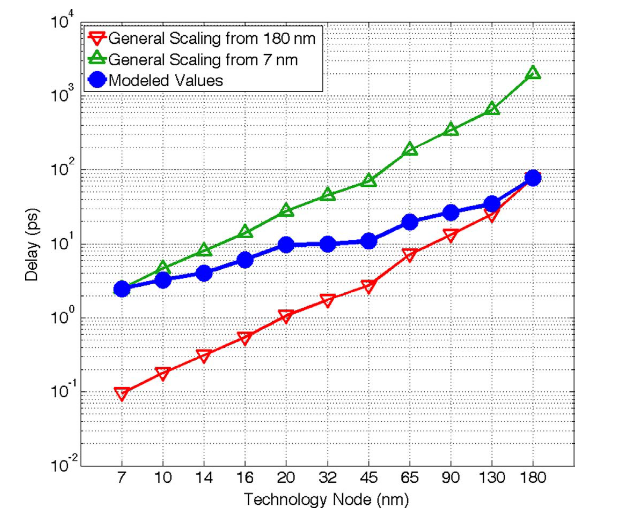
\includegraphics[width=0.6\textwidth]{scaling_delay_classical}
\caption{经典缩放方程预测的时延与 HSpice 仿真值的严重偏离\cite{stillmaker2017scaling}}
\label{fig:scaling_delay_classical}
\end{figure}

对此，转而采用 Stillmaker 与 Baas 提出的基于多项式拟合的深亚微米 CMOS 缩放模型\cite{stillmaker2017scaling}。该多项式框架基于海量 HSpice 仿真数据，将时延、能量与功耗映射为强关联于工艺参数与供电电压的多项式结构，提供了更可靠的跨尺度外推基准（图~\ref{fig:scaling_delay}\textendash\ref{fig:scaling_power}）：
\begin{equation}
\mathrm{DelayFactor}(V) = a_{d3} V^3 + a_{d2} V^2 + a_{d1} V + a_{d0}
\label{eq:delay_factor}
\end{equation}
\begin{equation}
\mathrm{EnergyFactor}(V) = a_{e2} V^2 + a_{e1} V + a_{e0}
\label{eq:energy_factor}
\end{equation}
\begin{equation}
\mathrm{PowerFactor}(V) = a_{p2} V^2 + a_{p1} V + a_{p0}
\label{eq:power_factor}
\end{equation}

\begin{figure}[H]
\centering
\begin{minipage}{0.32\textwidth}
\centering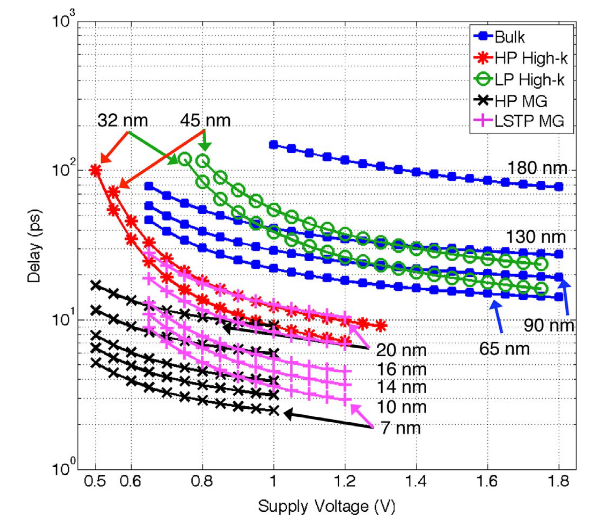
\includegraphics[width=\linewidth]{scaling_delay}
\caption{时延 \cite{stillmaker2017scaling}}
\label{fig:scaling_delay}
\end{minipage}
\hfill
\begin{minipage}{0.32\textwidth}
\centering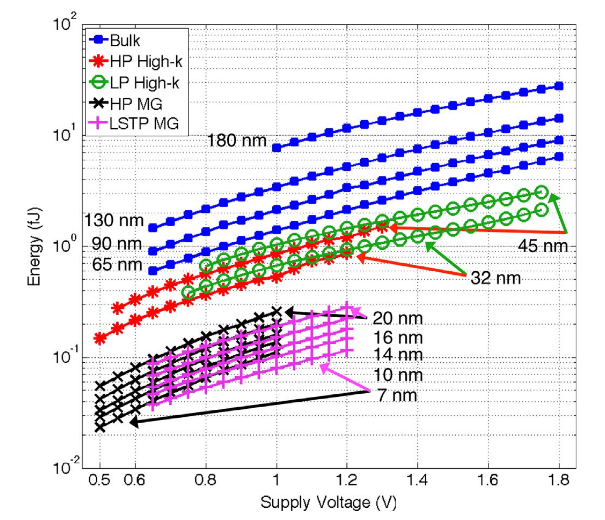
\includegraphics[width=\linewidth]{scaling_energy}
\caption{跃迁能量 \cite{stillmaker2017scaling}}
\label{fig:scaling_energy}
\end{minipage}
\hfill
\begin{minipage}{0.32\textwidth}
\centering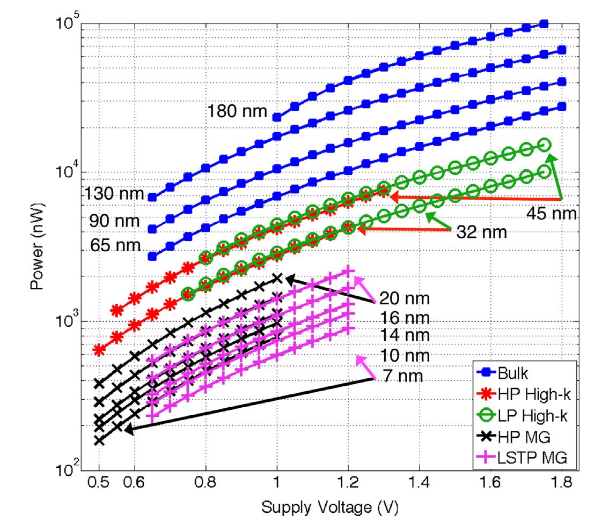
\includegraphics[width=\linewidth]{scaling_power}
\caption{随供电变化 \cite{stillmaker2017scaling}}
\label{fig:scaling_power}
\end{minipage}
\end{figure}

在具体的外推实施中，本文以前述 45\,nm Nangate 工艺库下获取的综合数据为映射锚点。面积缩放不依赖于供电电压，而是直接应用从 ITRS 技术路线图中推导出的几何均值比例因子（如表~\ref{tab:area_scaling} 与图~\ref{fig:scaling_area} 所示）：
\begin{equation}
A_x = A_y \cdot \mathrm{AreaScaleFactor}(y \to x)
\label{eq:area_scale}
\end{equation}

\begin{figure}[htbp]
\centering
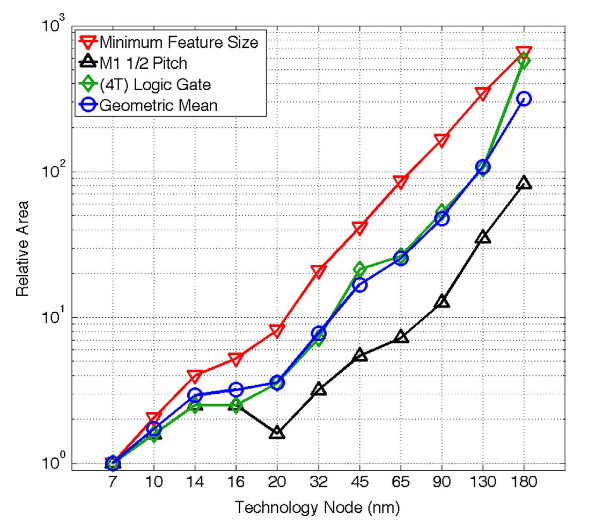
\includegraphics[width=0.6\textwidth]{scaling_area}
\caption{不同面积度量随工艺节点的相对缩放规律 \cite{stillmaker2017scaling}}
\label{fig:scaling_area}
\end{figure}

\begin{table}[htbp]
\centering
\caption{面积缩放因子选取参照表（局部，以各节点为基准）\cite{stillmaker2017scaling}}
\label{tab:area_scaling}
\small
\begin{tabular}{c|cccccc}
\toprule
基准 $\backslash$ 目标 & 45\,nm & 32\,nm & 20\,nm & 14\,nm & 10\,nm & 7\,nm \\
\midrule
45\,nm & 1 & 0.46 & 0.21 & 0.17 & 0.10 & 0.059 \\
\bottomrule
\end{tabular}
\end{table}

结合表~\ref{tab:scaling_coeffs} 中的 HP Multi-Gate 多项式系数，当时延与等效功耗自源工艺 $y$ 越迁至目标工艺 $x$ （伴随工作频率缩放）时，核心公式定格为：

给定起始工艺节点 \(y\) 与目标工艺节点 \(x\)，设起始节点的供电电压为 \(V_y\)，目标节点的供电电压为 \(V_x\)，则时延、能量与功耗的缩放公式分别为：

\begin{equation}
D_x = D_y \cdot \frac{\mathrm{DelayFactor}_x(V_x)}{\mathrm{DelayFactor}_y(V_y)}
\label{eq:delay_scale}
\end{equation}

\begin{equation}
E_x = E_y \cdot \frac{\mathrm{EnergyFactor}_x(V_x)}{\mathrm{EnergyFactor}_y(V_y)}
\label{eq:energy_scale}
\end{equation}

\begin{equation}
P_x = P_y \cdot \frac{\mathrm{PowerFactor}_x(V_x)}{\mathrm{PowerFactor}_y(V_y)}
\label{eq:power_scale}
\end{equation}

\begin{table}[H]
\footnotesize
\centering
\caption{HP Multi-Gate 工艺节点的缩放多项式系数\cite{stillmaker2017scaling}}
\label{tab:scaling_coeffs}
\begin{tabular}{c|cccc|ccc|ccc}
\toprule
 & \multicolumn{4}{c|}{时延系数} & \multicolumn{3}{c|}{能量系数} & \multicolumn{3}{c}{功耗系数} \\
节点 & \(a_{d3}\) & \(a_{d2}\) & \(a_{d1}\) & \(a_{d0}\) & \(a_{e2}\) & \(a_{e1}\) & \(a_{e0}\) & \(a_{p2}\) & \(a_{p1}\) & \(a_{p0}\) \\
\midrule
20 nm & --- & 34.63 & $-$66.37 & 41.15 & 0.373 & $-$0.1582 & 0.04104 & 2922 & $-$1286 & 299.9 \\
16 nm & --- & 24.80 & $-$47.52 & 28.87 & 0.2958 & $-$0.1241 & 0.03024 & 2133 & $-$882.6 & 197.7 \\
14 nm & $-$40.66 & 109.2 & $-$100.6 & 35.92 & 0.2363 & $-$0.09675 & 0.02239 & 1675 & $-$711 & 159 \\
10 nm & $-$34.95 & 93.65 & $-$85.99 & 30.4 & 0.2068 & $-$0.09311 & 0.02375 & 1456 & $-$621.6 & 143.8 \\
7 nm & $-$28.58 & 76.6 & $-$70.26 & 24.69 & 0.1776 & $-$0.09097 & 0.02447 & 1179 & $-$515.7 & 123.4 \\
\bottomrule
\end{tabular}
\end{table}

为了直观映射本文近似架构至商用极紫外光刻（EUV）主力节点，本文以 45\,nm HP High-K ($V_{\mathrm{DD}}{\approx}1.1\,\text{V}$) 作为宏观锚点，推演至目标工艺 7\,nm HP Multi-Gate ($V_{\mathrm{DD}}{\approx}0.7\,\text{V}$)。代入上述包含了对应节点系数与电压缩放的多项式拟合曲线，可获取固定的跨代际经验映射因子：面积缩放极值 $k_A \approx 0.059$、本征时延加速比 $k_D \approx 0.185$，以及频率等效功耗折损 $k_P \approx 0.142$。将 LETAM、TOSAM 与 ZBA-BM 所对应的 45\,nm 原生网表 PPA 表征数据全系代入关联缩放，预测生成的 7\,nm 映射基准如表~\ref{tab:7nm_mapped_ppa} 所示。

\begin{table}[htbp]
\centering
\caption{由 45\,nm 向 7\,nm 工艺的缩放映射评估}
\label{tab:7nm_mapped_ppa}
\small
\setlength{\tabcolsep}{5pt}
\begin{tabular}{lcccccc}
\toprule
\multirow{2}{*}{\textbf{架构配置}} & \multicolumn{3}{c}{\textbf{45\,nm 物理综合原生数据}} & \multicolumn{3}{c}{\textbf{7\,nm 极小尺寸映射数据} ($k_A, k_P, k_D$)} \\
\cmidrule(lr){2-4} \cmidrule(lr){5-7}
 & \textbf{面积}($\mu m^2$) & \textbf{功耗}($\mu W$) & \textbf{时延}(ns) & \textbf{面积}($\mu m^2$) & \textbf{功耗}($\mu W$) & \textbf{时延}(ns) \\
\midrule
\texttt{ExactSigned8bit}      & $314.14$ & $209.66$ & $1.30$ & $18.53$ & $29.77$ & $0.24$ \\
\texttt{ExactBooth8}  & $291.54$ & $276.71$ & $-$    & $17.20$ & $39.29$ & $-$    \\
\midrule
TOSAM(0,3)                    & $152.68$ & $114.10$ & $1.09$ & $9.01$  & $16.20$ & $0.20$ \\
TOSAM(1,4)                    & $207.75$ & $185.71$ & $1.41$ & $12.26$ & $26.37$ & $0.26$ \\
TOSAM(2,6)                    & $241.36$ & $241.23$ & $1.73$ & $14.24$ & $34.25$ & $0.32$ \\
TOSAM(3,7)                    & $291.54$ & $253.56$ & $2.05$ & $17.20$ & $36.01$ & $0.38$ \\
\midrule
\texttt{KMap\_4Row\_ZG} & $208.01$ & $234.29$ & $-$    & $12.27$ & $33.27$ & $-$    \\
ZBA-BM 0E4A                   & $197.11$ & $202.67$ & $-$    & $11.63$ & $28.78$ & $-$    \\
ZBA-BM 1E3A                   & $241.53$ & $230.62$ & $-$    & $14.25$ & $32.75$ & $-$    \\
ZBA-BM 2E2A                   & $263.34$ & $252.68$ & $-$    & $15.54$ & $35.88$ & $-$    \\
\midrule
LETAM(3,6)                    & $317.07$ & $234.99$ & $1.08$ & $18.71$ & $33.37$ & $0.20$ \\
\bottomrule
\end{tabular}
\end{table}

需要明确的是，此处多项式拟合本质建构在标准 FO4 门级电路之上，未针对具体布线层级极端 RC 互连线网损耗进行后仿真提取。故所得的各节点物理特质刻画具有强理论边界价值定量参考，而对实际脉动阵列互联瓶颈的最真实测算仍有赖全系统物理深层打样验证。

\clearpage
\section{结语}

\subsection{工作总结}
本文围绕面向大语言模型推理的近似计算加速架构，完成了从算子结构、RTL 实现、系统集成到应用级评估的跨层研究。首先，在算子层面选取 TOSAM、ZBA-BM 与 LETAM 三类具有代表性的近似乘法器进行分析与参数化实现。TOSAM 通过前导位检测、尾数截断与舍入重构形成可调精度路径，误差随参数提升呈单调收敛，其中 TOSAM$(3,7)$ 在全遍历统计中取得较低 RMSE，并在 ResNet-50 \texttt{conv1} 周期级测试中表现出最小输出扰动。LETAM 则利用高有效位提取和移位加法近似，在不同保留位宽下形成清晰的精度--硬件开销折中，LETAM(3,6) 在误差、时延与实现复杂度之间具有较均衡的特征。

其次，本文针对 Radix-4 Booth 近似乘法中的系统性偏差提出 ZBA-BM 结构。通过 K-Map 化简保留零编码守恒项，并对 Row-0 边界处 $\mu_{\text{row-0}}=-1/8$ 的固有偏差进行溯源，本文提出 Row-0 选择性部分积补偿（PPSC），在 $B_W=\mathtt{100}$ 时恢复 $-2A$ 部分积，使 ZBA-BM 0E4A、1E3A 与 2E2A 在 8 bit 全输入空间内均保持 $\mathrm{ME}\equiv0$。45\,nm Nangate 综合结果显示，ZBA-BM 2E2A、1E3A 与 0E4A 相对精确 Booth 基线分别实现 $9.7\%$、$17.2\%$、$32.4\%$ 的面积缩减和 $8.7\%$、$16.6\%$、$26.8\%$ 的动态功耗降低，说明局部补偿可以在较小硬件代价下修正均值偏差，但方差控制仍需依赖近似深度选择。

再次，本文将上述近似乘法路径接入 Chipyard/Gemmini 生成器，完成 PE 内乘法单元替换、Scala 生成逻辑适配、Verilator 裸机矩阵乘验证以及真实卷积层测试，形成了从 Chisel/RTL 到系统仿真的验证链路。ResNet-50 \texttt{conv1} 实测表明，TOSAM$(3,7)$ 的 RMSE 与 Frobenius 范数分别为 $0.4105$ 与 $183.9185$，优于 ZBA-BM 2E2A 的 $4.2046$ 与 $1883.6767$；而在面向长累加链的 Frobenius 尺度估计中，ZBA-BM 2E2A 依靠零均值特性，在长上下文 Attention 聚合参照点上获得低于 TOSAM$(3,7)$ 的预测 RMS 失真。该现象表明，短链路更受误差方差影响，长链路则对均值偏置更敏感。

最后，本文补充了 TinyLlama-1.1B 在 wikitext-2 test split 上的应用级困惑度评估，并采用 Stillmaker--Baas 深亚微米 CMOS 缩放模型进行 45\,nm 至 7\,nm 的跨工艺映射。PPL 结果显示，TOSAM$(3,7)$ 与 ZBA-BM 2E2A 分别为 $8.6207$ 与 $8.7807$，处于相近退化水平；ZBA-BM 1E3A 与无补偿配置退化明显，进一步说明零均值是必要条件而非充分条件。跨工艺外推则为近似乘法器在先进节点下的面积、功耗与时延趋势提供了统一参考。

\subsection{存在的不足与展望}
本文仍存在若干不足。其一，现有系统级周期仿真主要覆盖裸机矩阵乘与 ResNet-50 \texttt{conv1}，尚未完成完整 Transformer block 或端到端 LLM 推理链路的周期级验证；TinyLlama 实验采用 LUT 替换 \texttt{nn.Linear} 内部乘法，能够反映应用精度趋势，但不能完全等同于真实 Gemmini 执行路径。其二，误差建模主要基于独立同分布近似和 Frobenius 尺度估计，尚未充分刻画激活分布、量化尺度、残差连接和归一化操作对误差传播的调制作用。其三，输入零值门控与动态层级精度分配已完成结构设想，但尚缺少统一 RTL--PPA--应用精度口径下的闭环证据；跨工艺结果也仍属于模型外推，未包含版图布线、时钟树和温压角约束。

后续工作可从四个方向推进：第一，补齐 Transformer 层级和完整 GEMM 长链的周期级仿真，将 LUT 级精度评估与 Gemmini 实际执行路径对齐；第二，建立面向层敏感性的精度调度方法，使 TOSAM 的低方差特征、ZBA-BM 的零均值特征和 LETAM 的可配置截断能力能够按层、按矩阵规模或按输入分布协同选择；第三，探索 INT4 及更低位宽下的混合近似算子，并结合量化感知训练或轻量校准降低应用级退化；第四，推进后端物理实现验证，在真实布线、时钟门控、功耗门控和多工艺角条件下重新评估 PPA 收益。通过上述工作，可进一步判断近似乘法器在大模型推理硬件中的可部署边界，并为面向能效优化的张量加速器设计提供更完整的工程依据。

\clearpage


\reference
\end{document}
